\documentclass[a4paper, 11pt, twoside]{report}
% THIS FILE SHOULD BE COMPILED BY pdfLaTeX

% ----------------------   PREAMBLE PART ------------------------------
% ------------------------ ENCODING & LANGUAGES ----------------------

\usepackage[utf8]{inputenc}
%\usepackage[MeX]{polski} % Not needed unless You have a name with polish symbols or sth
\usepackage[T1]{fontenc}
\usepackage[english, polish]{babel}

\usepackage{amsmath, amsfonts, amsthm, latexsym} % MOSTLY MATHEMATICAL SYMBOLS
\usepackage{fancyvrb} % for full width verbatim blocks
\usepackage{placeins} % for creating floating barriers

\usepackage[final]{pdfpages} % INPUTING TITLE PDF PAGE - GENERATE IT FIRST!
\usepackage{biblatex}

\usepackage{listings} % code listing

\usepackage{commath} % various commands which can make writing math expressions easier --- documentation available at: https://ctan.gust.org.pl/tex-archive/macros/latex/contrib/commath/commath.pdf

\usepackage[hidelinks]{hyperref} % for hyperlinks, for example, urls, references to equations, entries in a bibliography --- hidelinks option removes rectangles around hiperlinks

% ---------------- MARGINS, INDENTATION, LINESPREAD ------------------

\usepackage[inner=20mm, outer=20mm, bindingoffset=10mm, top=25mm, bottom=25mm]{geometry} % MARGINS

\linespread{1.5}
\allowdisplaybreaks         % ALLOWS BREAKING PAGE IN MATH MODE

\usepackage{indentfirst}    % IT MAKES THE FIRST PARAGRAPH INDENTED; NOT NEEDED
\setlength{\parindent}{5mm} % WIDTH OF AN INDENTATION

%---------------- RUNNING HEAD - CHAPTER NAMES, PAGE NUMBERS ETC. -------------------

\usepackage{fancyhdr}
\pagestyle{fancy}
\fancyhf{}
% PAGINATION: LEFT ALIGNMENT ON EVEN PAGES, RIGHT ALIGNMENT ON ODD PAGES 
\fancyfoot[LE,RO]{\thepage} 
% RIGHT HEADER: zawartość \rightmark do lewego, wewnętrznego (marginesu) 
\fancyhead[LO]{\sc \nouppercase{\rightmark}}
% lewa pagina: zawartość \leftmark do prawego, wewnętrznego (marginesu) 
\fancyhead[RE]{\sc \leftmark}
\setlength{\headheight}{13.6pt}

\renewcommand{\chaptermark}[1]{\markboth{\thechapter.\ #1}{}}

% HEAD RULE - IT'S A LINE WHICH SEPARATES HEADER AND FOOTER FROM CONTENT
\renewcommand{\headrulewidth}{0 pt} % 0 MEANS NO RULE, 0.5 MEANS FINE RULE, THE BIGGER VALUE THE THICKER RULE

\fancypagestyle{plain}{
  \fancyhf{}
  \fancyfoot[LE,RO]{\thepage}
  
  \renewcommand{\headrulewidth}{0pt}
  \renewcommand{\footrulewidth}{0.0pt}
}

% --------------------------- CHAPTER HEADERS ---------------------

\usepackage{titlesec}
\titleformat{\chapter}
  {\normalfont\Large \bfseries}
  {\thechapter.}{1ex}{\Large}

\titleformat{\section}
  {\normalfont\large\bfseries}
  {\thesection.}{1ex}{}
\titlespacing{\section}{0pt}{30pt}{20pt} 
    
\titleformat{\subsection}
  {\normalfont \bfseries}
  {\thesubsection.}{1ex}{}

% ----------------------- TABLE OF CONTENTS SETUP ---------------------------

\def\cleardoublepage{\clearpage\if@twoside
\ifodd\c@page\else\hbox{}\thispagestyle{empty}\newpage
\if@twocolumn\hbox{}\newpage\fi\fi\fi}

% THIS MAKES DOTS IN TOC FOR CHAPTERS
\usepackage{etoolbox}
\makeatletter
\patchcmd{\l@chapter}
  {\hfil}
  {\leaders\hbox{\normalfont$\m@th\mkern \@dotsep mu\hbox{.}\mkern \@dotsep mu$}\hfill}
  {}{}
\makeatother

\usepackage{titletoc}
\makeatletter
\titlecontents{chapter}% <section-type>
  [0pt]% <left>
  {}% <above-code>
  {\bfseries \thecontentslabel.\quad}% <numbered-entry-format>
  {\bfseries}% <numberless-entry-format>
  {\bfseries\leaders\hbox{\normalfont$\m@th\mkern \@dotsep mu\hbox{.}\mkern \@dotsep mu$}\hfill\contentspage}% <filler-page-format>

\titlecontents{section}
  [1em]
  {}
  {\thecontentslabel.\quad}
  {}
  {\leaders\hbox{\normalfont$\m@th\mkern \@dotsep mu\hbox{.}\mkern \@dotsep mu$}\hfill\contentspage}

\titlecontents{subsection}
  [2em]
  {}
  {\thecontentslabel.\quad}
  {}
  {\leaders\hbox{\normalfont$\m@th\mkern \@dotsep mu\hbox{.}\mkern \@dotsep mu$}\hfill\contentspage}
\makeatother

% ---------------------- TABLES AD FIGURES NUMBERING ----------------------

\renewcommand*{\thetable}{\arabic{chapter}.\arabic{table}}
\renewcommand*{\thefigure}{\arabic{chapter}.\arabic{figure}}

% ------------- DEFINING ENVIRONMENTS FOR THEOREMS, DEFINITIONS ETC. ---------------

\makeatletter
\newtheoremstyle{definition}
{3ex}%                           % Space above
{3ex}%                           % Space below
{\upshape}%                      % Body font
{}%                              % Indent amount
{\bfseries}%                     % Theorem head font
{.}%                             % Punctuation after theorem head
{.5em}%                          % Space after theorem head, ' ', or \newline
{\thmname{#1}\thmnumber{ #2}\thmnote{ (#3)}}
\makeatother

\theoremstyle{definition}
\newtheorem{theorem}{Theorem}[chapter]
\newtheorem{lemma}[theorem]{Lemma}
\newtheorem{example}[theorem]{Example}
\newtheorem{proposition}[theorem]{Proposition}
\newtheorem{corollary}[theorem]{Corollary}
\newtheorem{definition}[theorem]{Definition}
\newtheorem{remark}[theorem]{Remark}

% --------------------- END OF PREAMBLE, USER COMMANDS --------------------------

\newcommand{\currentversion}{1.0}

\usepackage{csquotes}
\usepackage{graphicx}
\usepackage{float}
\usepackage{multirow}
\usepackage{multicol}
\usepackage{url} 
\usepackage{longtable}
\usepackage{array}
    \newcolumntype{S}[1]{>{\raggedright\arraybackslash}p{#1}}
    \newcolumntype{R}[1]{>{\raggedright\arraybackslash}m{#1}}
    \newcolumntype{P}[1]{>{\centering\arraybackslash}p{#1}}
    \newcolumntype{M}[1]{>{\centering\arraybackslash}m{#1}}

\graphicspath{{./assets}}
\addbibresource{references.bib}

% -------------------------- USER SETTINGS ---------------------------

\newcommand{\tytul}{Projekt aplikacji do generowania utworów fortepianowych \\ za pomocą sztucznej inteligencji}
\renewcommand{\title}{Project of Application for Piano Music Generation \\ by Artificial Intelligence Algorithms}


\newcommand{\type}{Engineer}
% \newcommand{\supervisor}{Jerzy Balicki DSc, Associate Professor}
\newcommand{\supervisor}{dr hab. inż. Jerzy Balicki, prof. uczelni}

\begin{document}
\sloppy
\selectlanguage{english}
\pagenumbering{gobble}

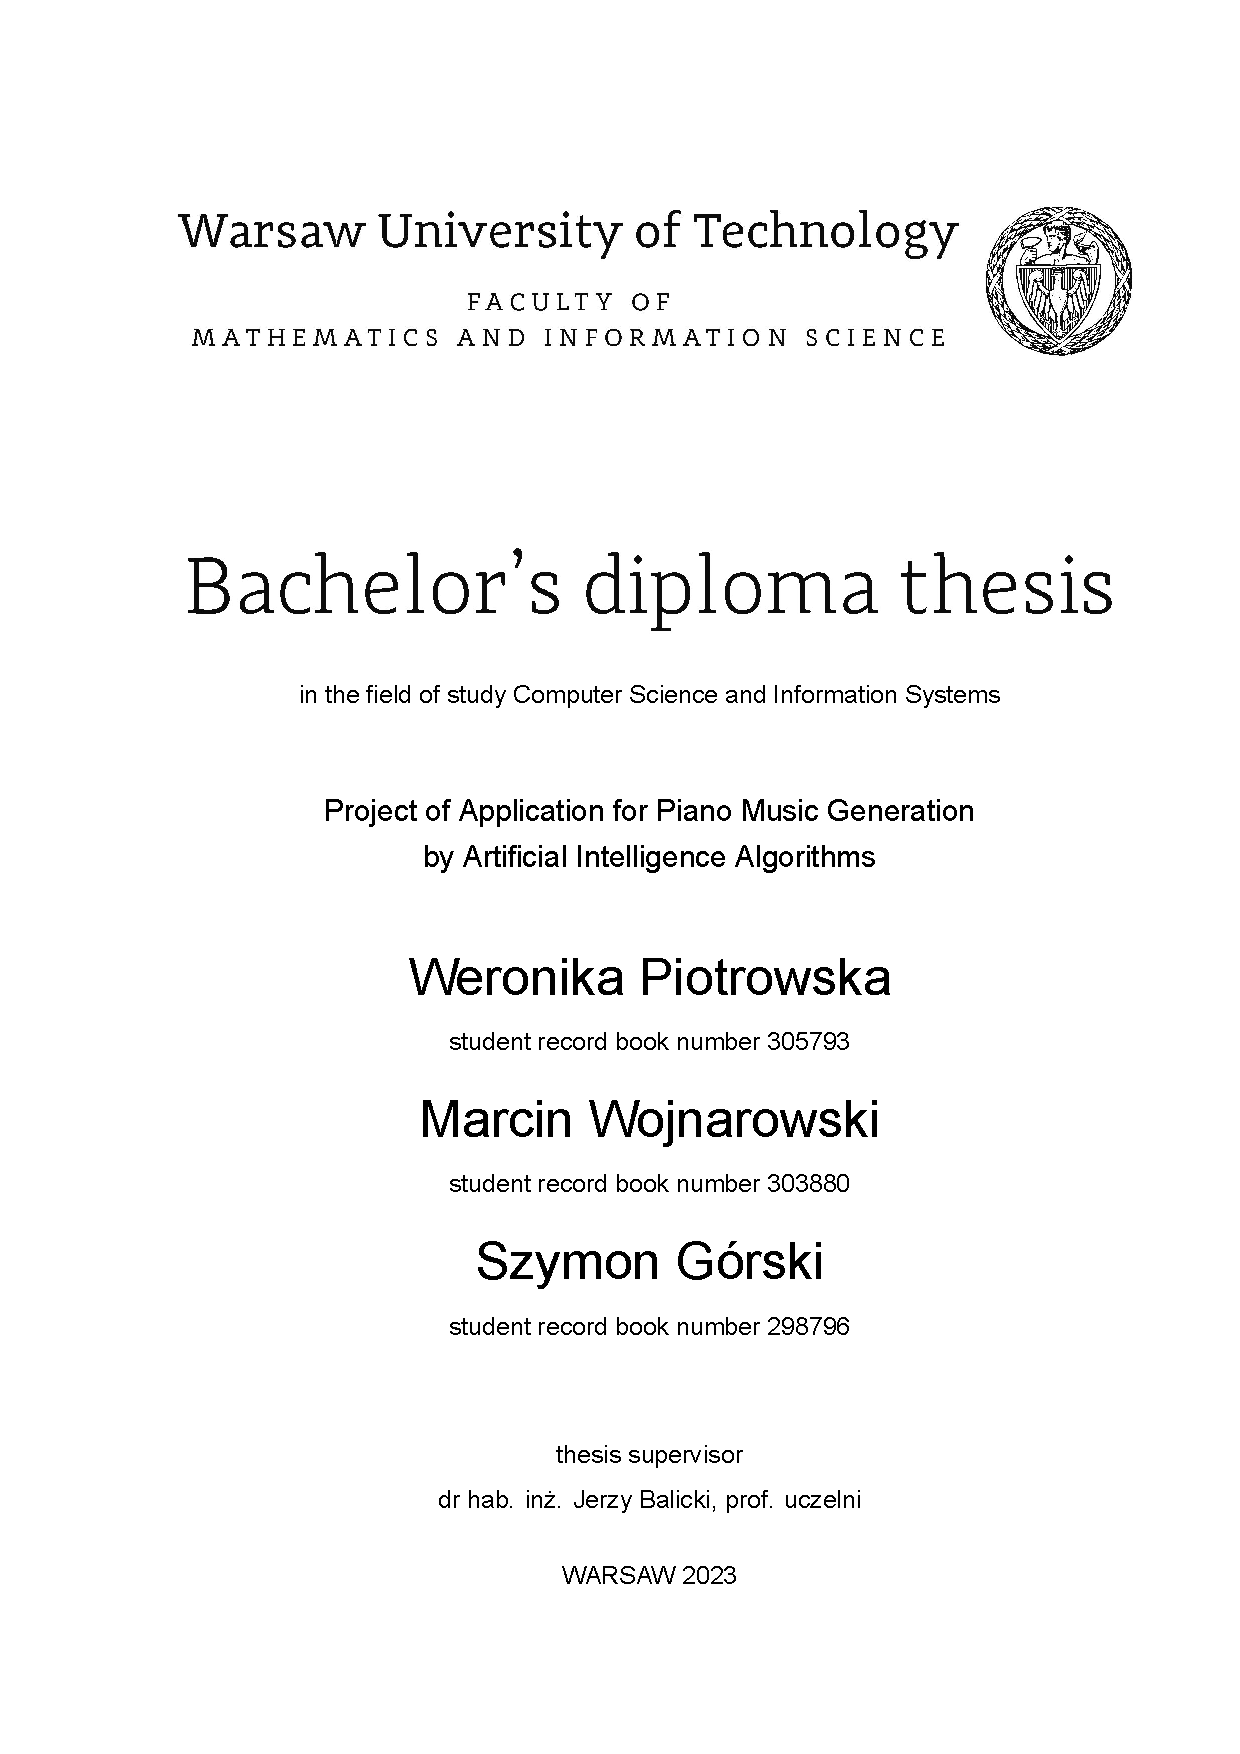
\includepdf[pages=-]{titlepage-eng}

\null\thispagestyle{empty}\newpage

\renewcommand{\figref}[1]{Figure \ref{fig:#1}}
\newcommand{\tabref}[1]{Table \ref{tab:#1}}

% ---------------------------- ABSTRACTS -----------------------------

{  \fontsize{12}{14} \selectfont
    \begin{abstract}

        \begin{center}
            \title
        \end{center}
        This bachelor's thesis presents an application focusing on the task of music generation using various models. Firstly, the authors present the problem statement alongside a dataset selection. The project is then outlined with mentions of its goals and specification. Implemented models are put forth with a brief description and motivation of choice. Later, the application used to interact with the models is presented along with its system architecture design. Finally, the solution is end-to-end evaluated and summarized with the authors' thoughts. \\

        \noindent \textbf{Keywords:} music generation, GAN, LSTM, MIDI
        % AI (Artificial Intelligence), GAN (Generative Adversarial Networks), LSTM (Long Short-Term Memory), Markov Chains, MIDI (Musical Instrument Digital Interface), Music Generation
    \end{abstract}
}

\null\thispagestyle{empty}\newpage

{\selectlanguage{polish} \fontsize{12}{14}\selectfont
    \begin{abstract}

        \begin{center}
            \tytul
        \end{center}
        Praca inżynierska prezentuje aplikację do generowania muzyki z wykorzystaniem wybranych modeli. Na początku autorzy przedstawiają omówienie problemu oraz wybór zbioru danych. Następnie zaprezentowany jest opis projektu wraz z jego celami i specyfikacją. Zaimplementowane modele są przedstawiane wraz z objaśnieniem i motywacją wyboru. Następnie opisywana jest aplikacja służąca do interakcji z modelami, wraz z jej architekturą systemu. Finalnie prezentowana jest ocena rozwiązania i podsumowanie. \\

        \noindent \textbf{Słowa kluczowe:} generowanie muzyki, sieć GAN, sieć LSTM, MIDI
    \end{abstract}
}

% ------------------- TABLE OF CONTENTS ---------------------

\null\thispagestyle{empty}\newpage
\selectlanguage{english} % for English

\tableofcontents
\thispagestyle{empty}
\newpage % IF YOU HAVE EVEN QUANTITY OD PAGES OF TOC, THEN REMOVE IT OR ADD \null\newpage FOR DOUBLE BLANK PAGE BEFORE INTRODUCTION

\null\thispagestyle{empty}\newpage
\pagestyle{fancy}
\pagenumbering{arabic}
\setcounter{page}{11}

% -------------------- THE BODY OF THE THESIS --------------------------------

\chapter*{Introduction}
\markboth{}{Introduction}
\addcontentsline{toc}{chapter}{Introduction}

This chapter presents the main objectives of this thesis as well as provides a summary of its content. \par


\section*{Motivation}

Despite Artificial Intelligence being known for its various applications in most Information Sciences, the topic of music processing is still an open problem being tackled from various angles. Though there are many existing approaches, they all suffer from drawbacks. Solutions range from consuming primitive music notes \cite{musenet} which are too restrictive in their output, to solutions that analyze raw audio spectrograms \cite{Forsgren_Martiros_2022} yielding distorted results. \par
Based on existing solutions for image and video processing, the authors implement and put in comparison three already existing generative models. The motivation behind the project is to explore ways of music generation with assistance of Machine Learning and create possibilities for other software engineers by creating a user-friendly application that shows the effects of the authors' work. \par


\section*{Goals}

This thesis aims at presenting the implementation and evaluation of the application developed by authors, dedicated to generating music. This goal is achieved by providing documentation of developed software, including descriptions of an executive summary, and functional requirements, along with user stories, use cases, and non-functional requirements divided into URPS categories. Additionally, the authors document the development of the application in form of a scope-of-work as well as a SWOT risk analysis. The division of tasks among authors was presented in Appendix \ref{app:work}. The work of the application is evaluated by comparison of algorithms used concerning results obtained. \par
An optional goal of the application development is to generate a piece of music that is indistinguishable from the original dataset. However, the assessment of this objective is mostly based on a subjective impression of an individual and should not be a subject of evaluation by numerical means. Therefore, it is not the point of focus of this thesis. \par


\section*{Thesis content}

In the first chapter authors describe a selection of data used along software development, motivations supporting the choice, and means of connection among different formats of data representation. The next segment is devoted to a presentation of models used in the application. The third part of the thesis provides a detailed specification of the software created by the authors. Chapter four presents the evaluation of the program using selected metrics as well as exemplary compositions created with it. Finally, the authors summarize the process of creation of the application and the thesis itself. \par



\chapter{Selected data} \label{chapter:selected_data}

Artificial Intelligence algorithms provide output requested by its user based on information obtained and analyzed earlier in a process of training. The selection of data is therefore a crucial step in achieving satisfactory results during software runtime. Feeding an AI algorithm with data should be preceded by its formatting, usually in a numerical form. This is often a challenge as software developers must decide which information to include in a model input and how to structure it to make algorithms efficient. \par


\section{Musical Instrument Digital Interface} \label{chapter:MIDI}

Musical Instrument Digital Interface is a multi-layer standard of information dispatch between audio devices defining connectors, interfaces, and protocols used by them. The key goal of introducing it was to unify communication means between musical equipment of different manufacturers \cite{MIDI_history}. MIDI focuses on data patterns necessary to emit and retrieve digitalized music in real time. It encodes musical notation rather than stores audio itself allowing for lossless yet extremely compact data representation. \par
MIDI was proposed in 1981 by the president of Roland corporation Ikutaro Kakehashi and standardized four years later with the acclamation of major digital audio device manufacturers \cite{MIDI_history}. In 1991, the MIDI File standard was introduced. It allowed to store streams of signals in a static file by adding delta-time labels to consecutive events \cite{MIDI1_file}. The most current revisions of these specifications were published in 1996 \cite{MIDI1_spec}, followed by next-generation standard MIDI 2.0, presented in 2020 by the MIDI Manufacturers Association along with the Association of Musical Electronics Industry \cite{MIDI2}. \par

\subsection{Standard description} \label{chapter:standard}

MIDI files (of extension \texttt{.mid} or \texttt{.midi}) can be of three format types:

\begin{itemize}
    \item \textit{Type 0}, in which all information is stored on a single track,
    \item \textit{Type 1}, which stores multiple (at least one) tracks with information,
    \item \textit{Type 2}, which stores independent single-track patterns.
\end{itemize} \par

In the planning phase of the software application authors decided to focus on \textit{format 1} files due to their straightforward representation of polyphony in both reading and separating melody lines. This format is described below. \par
MIDI files of format 1 are divided into 'chunks' beginning with a file header and ending with the dedicated \texttt{FF 2F 00} \textit{End of track} message. The first chunk begins with the \textit{MThd} file header and specifies a format type, number of tracks, and number of ticks per beat, which is the density of information notation. The last one is hard coded for the whole file, whereas playback tempo (expressed in microseconds) may change independently over time. \par
All track chunks begin with the \textit{MTrk} track header. The first track always consists of meta-messages only which cover information about channel-independent meta-events, like time signatures and tempo changes. The following tracks include series of messages emulating consecutive events from real-time signal transmissions. \par
As messages in MIDI files are stored using a streaming format, they have additional timestamps representing the number of ticks that elapsed from the last event (in a particular track). It creates a pipeline in which no intermediate state can be read without full knowledge of previous events. Moreover, they are chronological within a track only. To correctly reproduce events from different tracks, one must read the whole file before a playback even begins, therefore the possibility of on-demand partial streaming is not supported (in contrast to audio compression formats e.g., MP3). \par
Musical notes are assigned MIDI notes as their frequency progresses. They are stored as integers from 0 for the C-1 note (equivalent to 8 Hz) to 127 for the G\#9 note (equivalent to 13,290 Hz), twelve pitches for each octave (compare with Appendix \ref{app:notes}). Despite being stored in eight-bit bytes, most numbers use seven bits of representation (as the first bit is dedicated to differentiating them from event codes) with calculus adjusted for multibyte integers accordingly. \par
Messages informing about changes in playback have the following content:

\begin{itemize}
    \item Delta-time measured from last event (of variable length),
    \item Event code containing 'note on' \texttt{8} or 'note off' \texttt{9} command with the number of a channel \texttt{0-F} (1 byte),
    \item The number of a note \texttt{00-8F} (1 byte),
    \item Velocity representing dynamics or amount of pressure used to perform the action \texttt{00-8F} \\ (1 byte).
\end{itemize} \par

For example, \texttt{83 00 92 40 60} message should be understood as presented in \tabref{message}. \par

\begin{table}[H]
    \centering
    \caption{Interpretation of a MIDI message} \vskip16pt
    \label{tab:message}
    \begin{tabular}{ | M{3cm} S{6cm} | }
        \hline
        \setlength{\baselineskip}{12pt}\small Value (HEX) & \setlength{\baselineskip}{12pt}\small Description                  \\ \hline
        \setlength{\baselineskip}{12pt}\texttt{83 00}     & \setlength{\baselineskip}{12pt}After 384 ticks                     \\
        \setlength{\baselineskip}{12pt}\texttt{92}        & \setlength{\baselineskip}{12pt}turn on in Channel 2                \\
        \setlength{\baselineskip}{12pt}\texttt{40}        & \setlength{\baselineskip}{12pt}note number 64 (note E4)            \\
        \setlength{\baselineskip}{12pt}\texttt{60}        & \setlength{\baselineskip}{12pt}using forte (96 units of) dynamics. \\ \hline
    \end{tabular}
\end{table}

An event code can be omitted if matches the code from the previous message. Moreover, setting note velocity via 'note on' to 0 is often used instead of 'note off' code, which is formally acceptable but may cause sound differences for some instruments \cite{MIDI1_spec}. \par

\subsection{Possibilities and limitations}

MIDI provides the platform for content creators to efficiently digitalize music. Due to the widespread usage of the format, hundreds of thousands of '.mid' files have become available online\footnote{The largest free-to-use MIDI databases (\textit{BitMidi}, \textit{Midis Free}) store over one hundred thousand MIDI files each (as of January 2023).}. Numerical representation of information yields possibilities in Machine Learning and Artificial Intelligence data processing and interpretation. \par
The versatility of the standard is its strength and weakness at the same time. Some authors utilizing the format, as well as some audio equipment, do not use dedicated types of messages. Examples include 'note on' and 'note off' messages described in Sect. \ref{chapter:standard} or creating additional tracks to pass authors, a source, or copyrights information in their titles. Moreover, the representation itself is not unique, allowing some configurations to be presented in multiple ways, e.g., when one note ends and the other begins at one track at the same time, it is possible to either turn off the first note and then turn on the second one or turn on the second note and then turn off the first one \cite{MIDI1_spec}. These ambiguities enforce additional steps and checks when designing decoders of MIDI files. \par


\section{Selected dataset for piano music composition}

To create a dataset used in the project, authors examined multiple resources of MIDI files available online. The final dataset is a selection of records from three of these databases. The main criterium of file choice is to provide a collection of compositions by the same author for the same instrument (to increase the chance of structural pattern recognition). The composer should be both popular and prolific to allow the set to be of satisfactory size. The authors chose Johann Sebastian Bach as the author of the selected files. \par

\subsection{Johann Sebastian Bach}

Johann Sebastian Bach (1685 - 1750) was a Baroque-era German composer known for devoting particular attention to the structure of his compositions. Bach's works often have the same, transformed structures supported by mathematical concepts \cite{Bach}. For example, \textit{Canon Duplex a 4}, BWV 1087 can be written and then read from a hollowed out Möbius strip \cite{Mobius}. Authors believe that compositions strongly tied to mathematics may have a higher factor of replicability when analyzed by Artificial Intelligence. \par

\subsection{Overview of the dataset}

\begin{figure}[t]
    \centering
    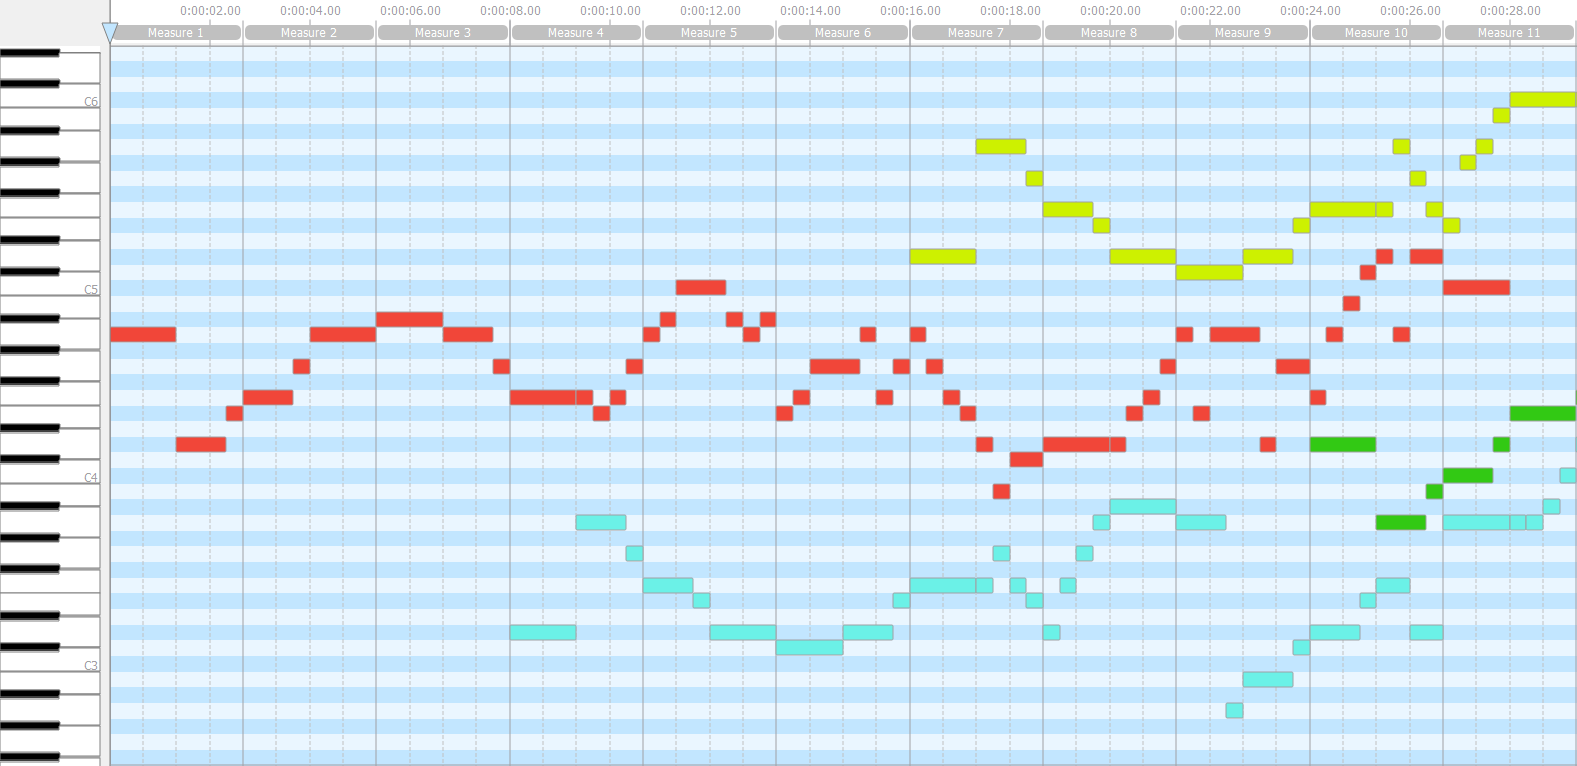
\includegraphics[width=0.98\textwidth]{assets/midieditor.png}
    \caption{The first eleven measures of \textit{Contrapunctus 5}, BWV 1080 as decoded from a MIDI file \texttt{bwv1080-cnt1.mid} in external application \textit{MidiEditor}. Different colors represent tracks of notes}
    \label{fig:scr_midieditor}
\end{figure}

\begin{figure}[t]
    \centering
    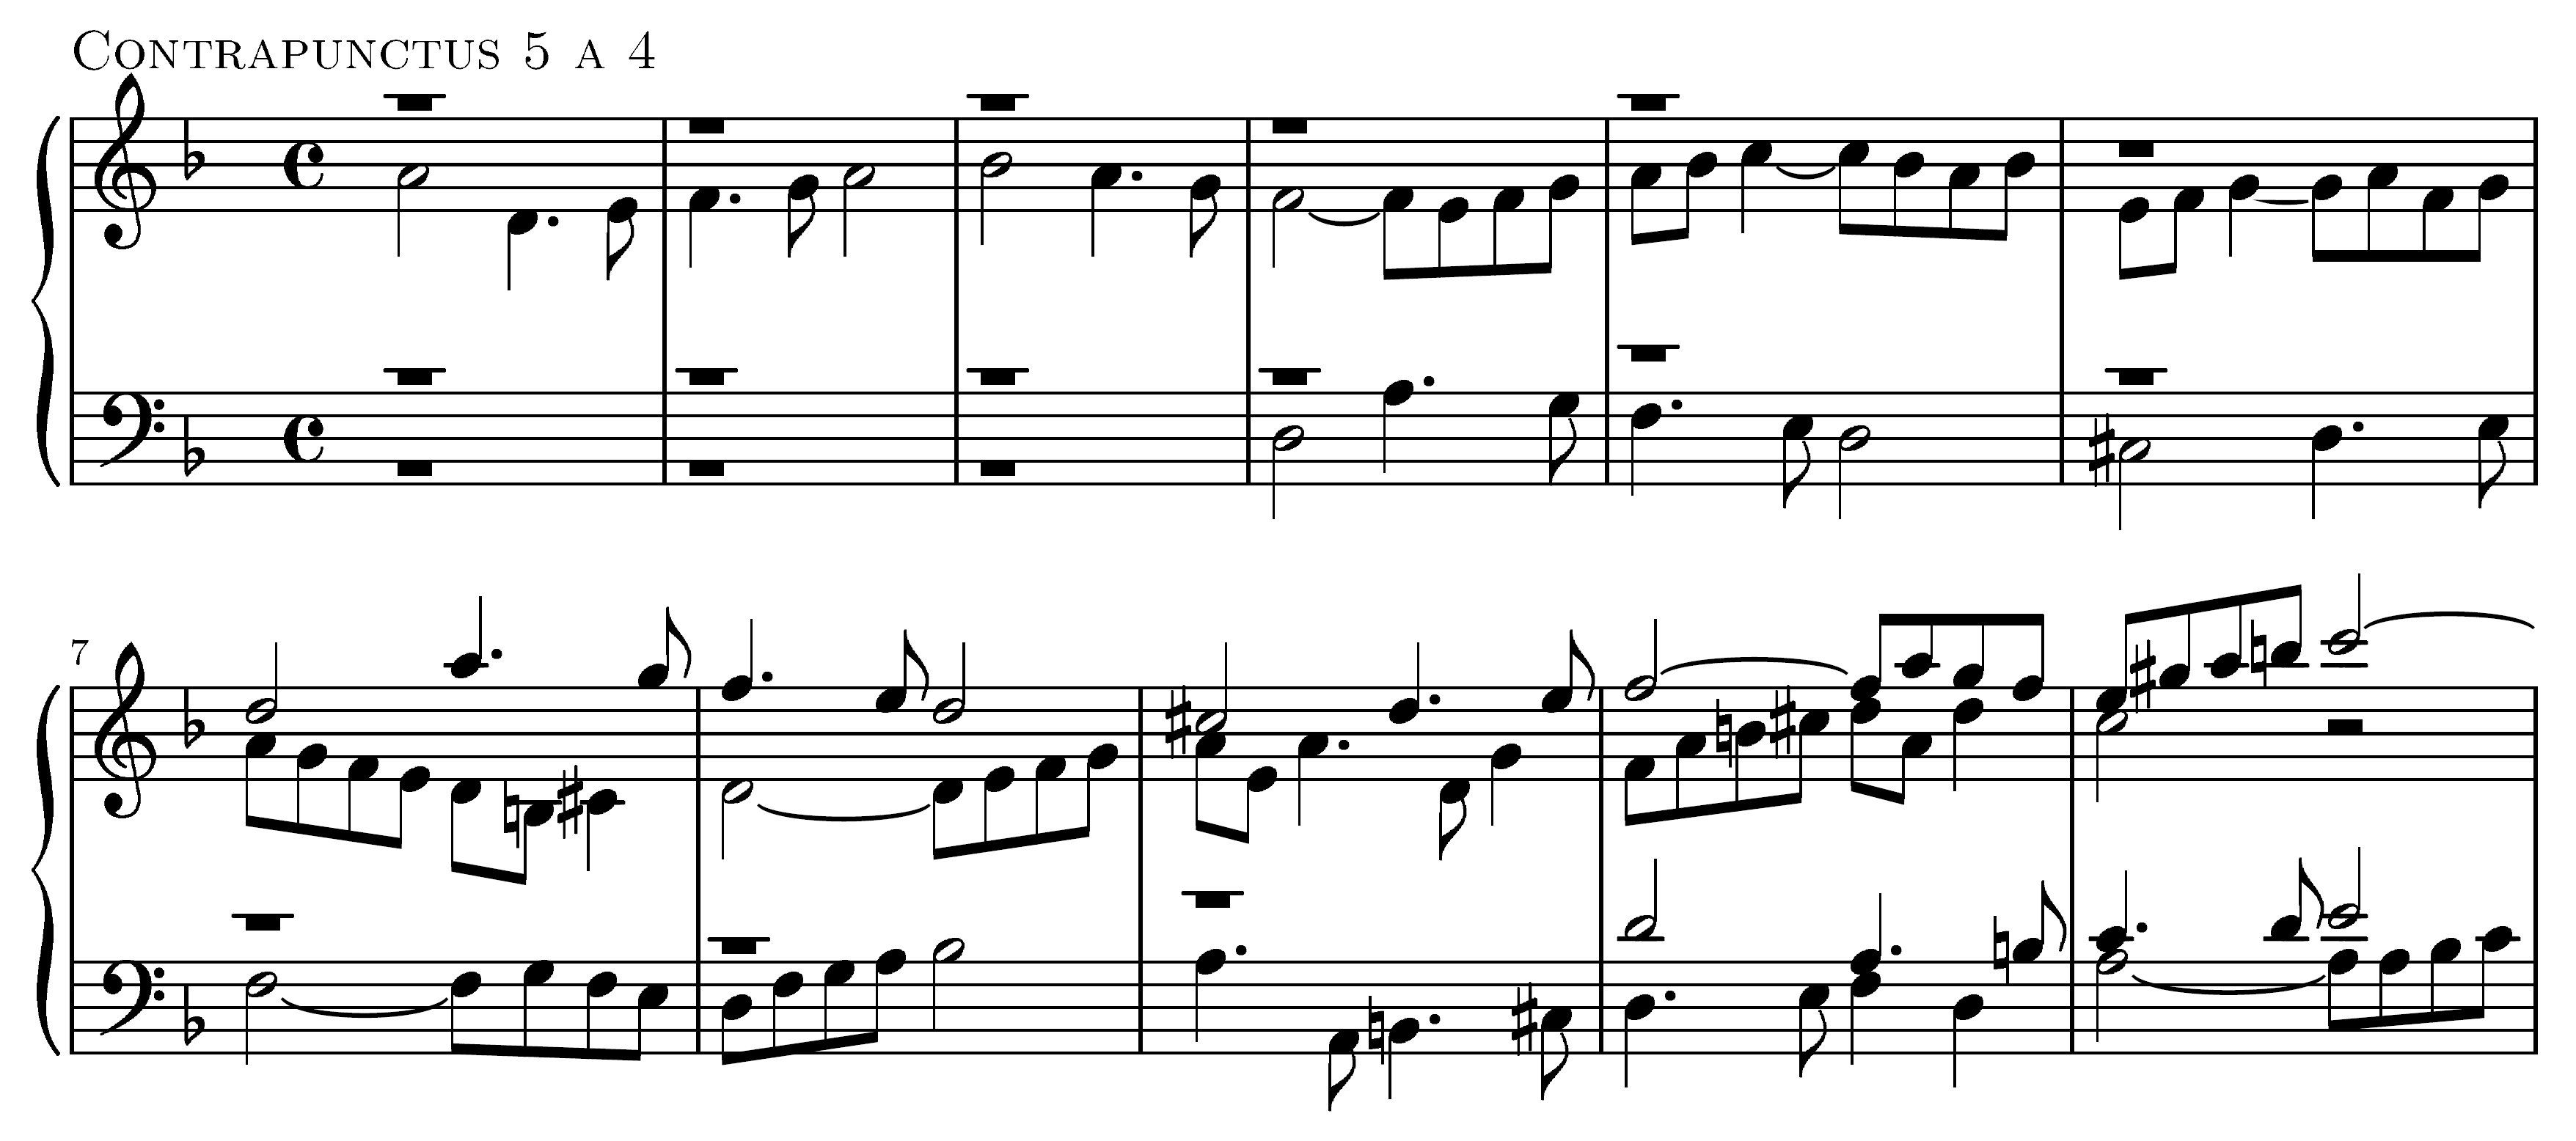
\includegraphics[width=1\textwidth]{assets/bach_sample.png}
    \caption{The first eleven measures of \textit{Contrapunctus 5}, BWV 1080 in its original notation. Score digitized by T. Knigge}
    \label{fig:scr_contra5}
\end{figure}

Most large databases of MIDI files include direct translations of audio compression volume levels to MIDI notes, yielding most of the keyboard turned on since sound effects of instruments span across a wide range of frequencies. Despite proper velocities setup, the amount of unnecessary information included makes these files unusable in deep learning. An example of such a dataset is presented in \cite{MIDI_dirty}. \par
It is considered very hard to translate an audio recording back to original sheet music and impossible as of now to automatically separate lines of polyphony due to their interlocking. Most high-quality files storing music notation, e.g., MIDI, PDF, contain data either once manually presented using means of notation (e.g., sheet music or dedicated software), or captured automatically but manually corrected later. Figure \ref{fig:scr_midieditor} presents a decoded MIDI file from the dataset with its notes' heights plotted against time (compare with the original score presented in Figure \ref{fig:scr_contra5}). \par

\subsection{Specification of selected dataset} \label{sec:data_spec}

The dataset used by authors in the development of the application consists of 184 records from three databases:

\begin{enumerate}
    \item \textit{A Johann Sebastian Bach Midi Page} by B. Travis \cite{MIDI_central},
    \item \textit{Dave's J.S. Bach Page} by D. J. Grossman \cite{MIDI_Dave},
    \item \textit{Large collection of Classical MIDI of Bach's music} by kunstderfuge.com \cite{MIDI_kunst}.
\end{enumerate} \par

All files contain 154 original compositions by Johann Sebastian Bach for fortepiano and harpsichord (see Vocabulary). The works included in the dataset are:

\begin{itemize}
    \item 15 \textit{Two-voice Inventions}, \small BWV 772-786 (15 files), \normalsize
    \item 15 \textit{Three-voice Sinfonias}, \small BWV 787-801 (15 files), \normalsize
    \item \textit{Four Duets}, \small BWV 802-805 (4 files), \normalsize
    \item 6 \textit{English Suites}, \small BWV 806-811 (48 files), \normalsize
    \item 24 Preludes and Fugues from \textit{The Well-tempered Clavier} (Book I), \small BWV 846-869 (24 files), \normalsize
    \item 24 Preludes and Fugues from \textit{The Well-tempered Clavier} (Book II), \small BWV 870-893 (24 files), \normalsize
    \item \textit{Aria} and 30 Variations from \textit{Goldberg Variations}, \small BWV 988 (31 files), \normalsize
    \item 13 Counterpoints from \textit{The Art of Fugue}, \small BWV 1080 (13 files), \normalsize
    \item 22 other works \small (10 files). \normalsize
\end{itemize} \par

The detailed list of work titles, corresponding MIDI files, and their authors is included in Appendix \ref{app:dataset}. \par


\section{Remarks and conclusions}

The creation of MIDI files with the concept of passing data via messages is not straightforward. Not all creators manually utilizing the format put enough effort to meet the documentation standards, therefore low-quality files sometimes yield errors while being decoded.  \par
Fidelity to the original sheet music is not fully measurable employing hearing, therefore some datasets contain automatically generated files with an extremely different representation of compositions. Whereas some functions do not suffer from such a change, it is a crucial point in AI to secure as high dataset quality as possible. Therefore, the selection of files was conducted rigorously at the cost of the size of the set. For the application to handle files of any quality provided by users, authors made efforts to nullify the most popular errors appearing in MIDI files. \par



\chapter{Selected models}

The client application has access to a chosen subset of models. This section is devoted to the description of chosen Machine Learning models and reasons why they are suitable for the problem of music generation. \par


\section{Generative Adversarial Networks}

Generative Adversarial Networks (GANs) were published by Ian Goodfellow et al. in 2014 \cite{GAN_arxiv}. This architecture consists of two models: a \textit{generator} which generates fake samples and a \textit{discriminator} which discriminates between real and fake samples. Model processing consists of training the generator and the discriminator simultaneously, and the accuracy of one of them is dependent on the failure of another. In the perfect scenario, the generator finds a way to mimic real samples, thus the discriminator cannot distinguish them, having 50\% accuracy. \par
The input data used to train a GAN is a set of two-dimensional boolean matrices, which represent a MIDI file with joined channels (see Section \ref{chapter:MIDI}). \par

\subsection{Discriminator model}
The discriminator model is a binary classifier with convolution layers. Its purpose is to distinguish between real and fake samples, labeled as 1 and 0, respectively. However, what needs to be achieved is a situation where the discriminator fails to differentiate between these categories. Thus, its architecture should not be overcomplicated, so that it lets the generator achieve decent results. \par
The input for the model is a two-dimensional array with a fixed size. The model consists of the layers shown in Figure \ref{fig:disc-arch}, with the addition of batch normalization and dropout layers. \par

\begin{figure}
    \centering
    \begin{tiny}
        \begin{BVerbatim}
            Model: "discriminator"
            _________________________________________________________________
            Layer (type)                Output Shape              Param #
            =================================================================

            gaussian_noise (GaussianNoi  (None, 128, 512)         0
            se)

            conv1d (Conv1D)             (None, 16, 256)           393472

            leaky_re_lu (LeakyReLU)     (None, 16, 256)           0

            conv1d_1 (Conv1D)           (None, 2, 256)            196864

            leaky_re_lu_1 (LeakyReLU)   (None, 2, 256)            0

            flatten (Flatten)           (None, 512)               0


            dense (Dense)               (None, 1)                 513

            =================================================================
            Total params: 590,849
            Trainable params: 0
            Non-trainable params: 590,849
            _________________________________________________________________
        \end{BVerbatim}
    \end{tiny}
    \caption{GAN discriminator model architecture}
    \label{fig:disc-arch}
\end{figure}

The discriminator is evaluated against shuffled real samples from the dataset and fake samples generated by the generator. \par

\subsection{Generator model}

The generator model has a more complicated architecture since it uses several deconvolutional layers to generate samples from latent space. The generator's input is an array of randomized points in latent space and as an output, it produces a two-dimensional boolean array, which resembles a MIDI file representation. The architecture of the generator is shown in Figure \ref{fig:gen-arch}, with the addition of dropout, batch normalization, and reshape layers. \par

\begin{figure}
    \centering
    \begin{tiny}
        \begin{BVerbatim}
            Model: "generator"
            _________________________________________________________________
            Layer (type)                Output Shape              Param #
            =================================================================
            dense_1 (Dense)             (None, 1024)              66560

            leaky_re_lu_2 (LeakyReLU)   (None, 1024)              0

            conv1d_transpose (Conv1DTra  (None, 32, 512)          393728
            nspose)

            leaky_re_lu_3 (LeakyReLU)   (None, 32, 512)           0

            conv1d_transpose_1 (Conv1DT  (None, 256, 256)         393472
            ranspose)

            leaky_re_lu_4 (LeakyReLU)   (None, 256, 256)          0

            gaussian_noise_1 (GaussianN  (None, 256, 256)         0
            oise)

            activation (Activation)     (None, 128, 512)          0

            =================================================================
            Total params: 855,808
            Trainable params: 854,784
            Non-trainable params: 1,024
            _________________________________________________________________
        \end{BVerbatim}
    \end{tiny}
    \caption{GAN generator model architecture}
    \label{fig:gen-arch}
\end{figure}\par

Training of the generator is evaluated solely by the discriminator. The discriminator's weights are frozen, and the generator's output is passed to the discriminator labeled as \textit{real} samples. If the discriminator labels these samples as \textit{real}, it means that the generator is capable of generating non-distinguishable samples. \par

\subsection{Complete GAN model}

The final GAN model assembles the generator and the discriminator, adds a \textit{}{Flatten layer}, and defines a loss function and an optimizer. The chosen loss function is binary cross-entropy and the \textit{}{Adam} optimizer is used. Assuming that latent points are randomly generated, the generator should produce different samples each time, unless it is limited by latent space size. Visualization of GAN architecture is shown in Figure \ref{fig:GAN}. \par

\begin{figure}[H]
    \begin{center}
        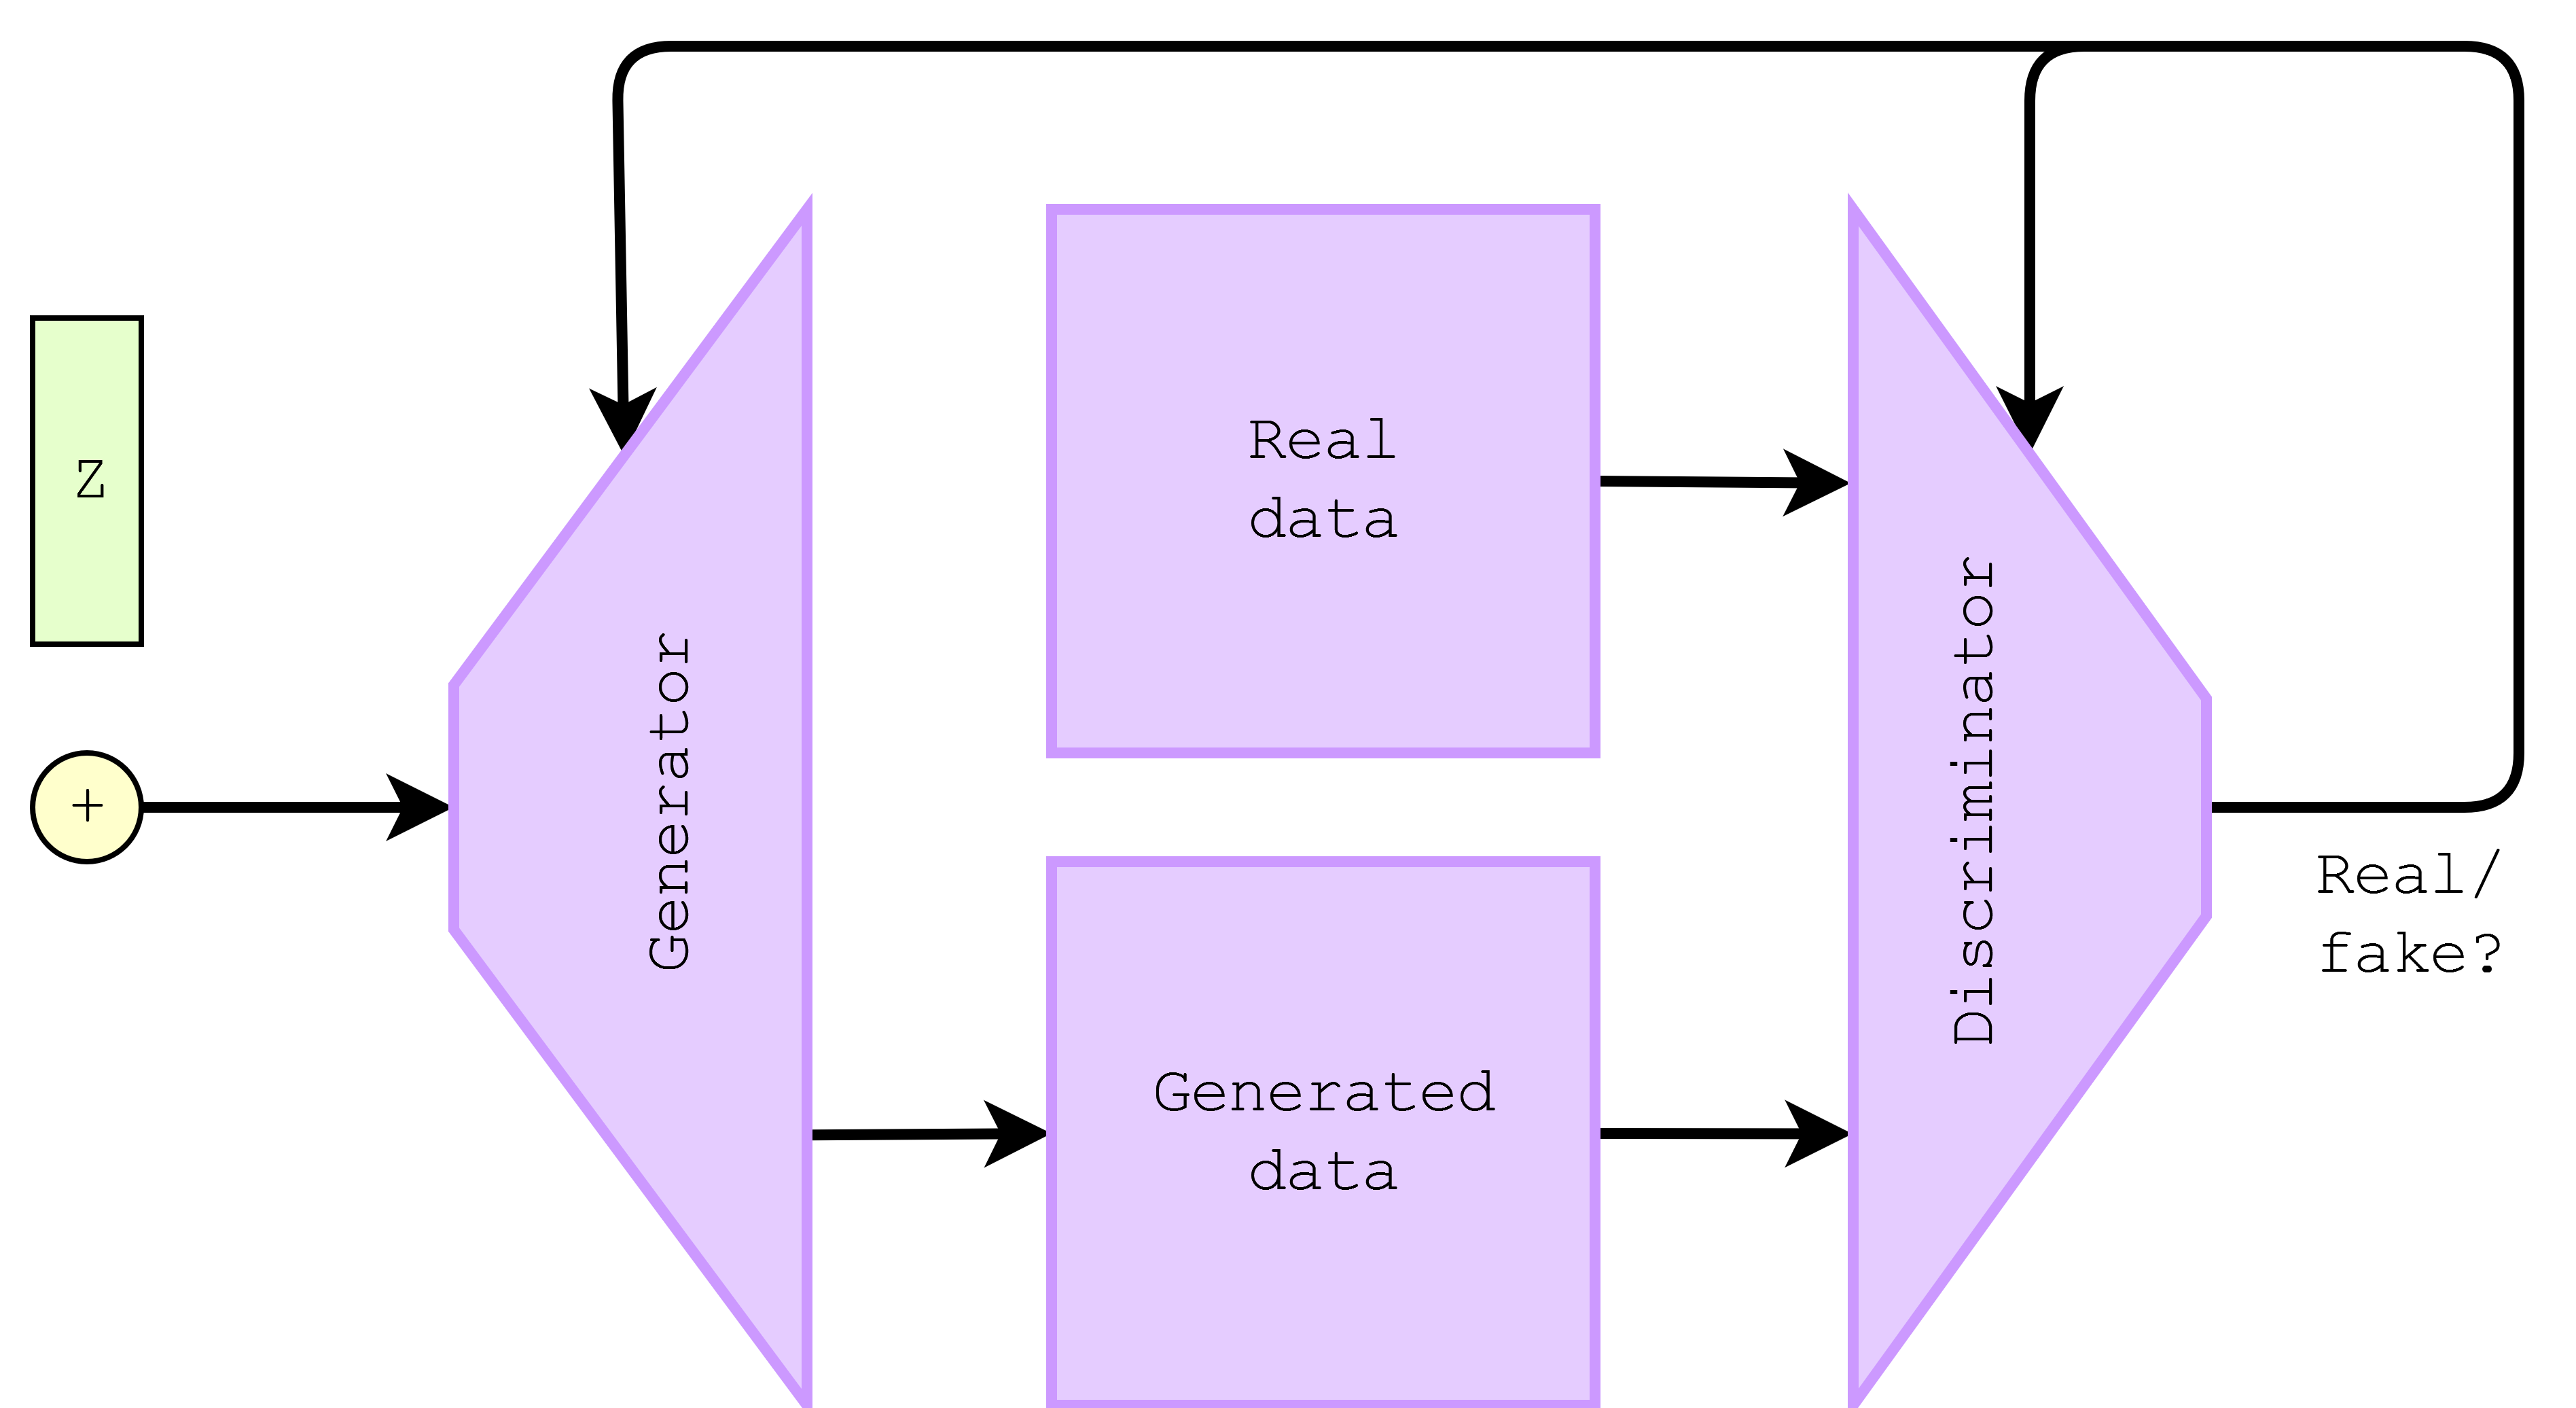
\includegraphics[width=0.7\textwidth]{assets/GAN_v2.png}
        \caption{Complete GAN model architecture. $Z$ represents a latent space, $+$ represents noise added}
        \label{fig:GAN}
    \end{center}
\end{figure}

Training of the entire model consists of three repeatable steps:

\begin{enumerate}
    \item Training the discriminator on real and fake samples,
    \item Freezing the discriminator and training the generator,
    \item Evaluating the generator based on a discriminator's classification.
\end{enumerate} \par

GANs have been widely used in Computer Vision and for a long time were considered a state-of-the-art solution \cite{GAN_SOTA}. Since music generation can be performed on arrays similar to images, the GAN model should perform similarly on processed MIDI samples as it does on images. Hence, using a GAN in the project is a reasonable choice, which may lead to satisfactory results. \par


\section{Long Short-Term Memory}

Long Short-Term Memory (LSTM) Networks are a type of Recurrent Neural Networks, which means they consume a continuous sequence of inputs one by one and aim to produce some requested output based on the current progress in the sequence. In other words, LSTMs operate on time-series data which is exactly what music is. \par
The main computation unit of an LSTM network is the \textit{LSTM unit} (\figref{lstm_unit}). It is responsible for computing two outputs based on three inputs. As input, it accepts long-term memory, short-term memory, and the current input. Given these, by using the following three gates the output is computed:

\begin{itemize}
    \item \textit{Forget gate} -- calculates how much of the long-term memory should be preserved,
    \item \textit{Input gate} -- calculates additional long-term memory,
    \item \textit{Output gate} -- calculates the final unit output using all updated inputs.
\end{itemize} \par

This produces two outputs. One of the outputs forms a memory (state) which is fed to the next LSTM unit as the long-term memory. The other output has two roles: the direct output of this unit and the input to the next LSTM unit as the short-term memory. Stacking many such units creates an LSTM network. This propagated memory allows this network to produce outputs based on events that happened in the past. \par

\begin{figure}
    \centering
    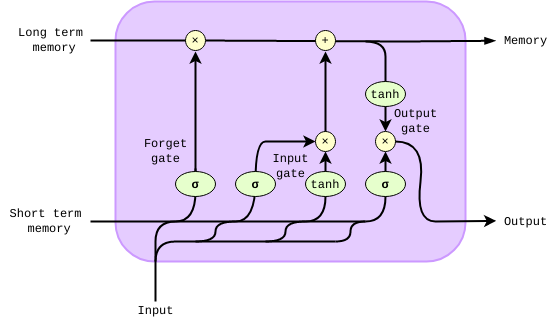
\includegraphics[width=0.7\textwidth]{lstm_unit.png}
    \caption{Single LSTM unit propagating the long- and short-term memory state. $\sigma$ represents the sigmoid function, $\tanh$ represents the hyperbolic tangent function. The location of trainable weights and biases is omitted for clarity}
    \label{fig:lstm_unit}
\end{figure}

LSTMs are a popular choice for music generation because of the presented properties. There are many variations of RNNs, and LSTM is only one of them. This choice was backed by LSTM's wide presence in the deep learning space and its general applicability to various sets of problems. There have been many attempts at using LSTMs for music generation \cite{lstm_arxiv}. Implementations usually differ in the input and the configuration of layers and hyperparameters used. \par

\subsection{Input/output shape}

\newcommand{\lstmseqlen}{25}

The discussion of shape of data is especially important as it is what affects the generation performance the most. \par
The class of RNN models has the advantage of not depending on the sequence length allowing for variable-sized inputs. However, they are still constrained to the shape of data in each sequence item. The chosen shape for the LSTM model is an array of active notes across the range of all possible notes. Additionally, since the model predicts the next chord based on $n$ previous ones, an appropriate $n$ integer must be picked. From testing, it was inferred that a comfortable value for $n$ giving enough context for the network to predict the next chord is $\lstmseqlen$. Thus the input to the network is a $\{0, 1\}^{\lstmseqlen \times 128}$ matrix with a $1$ when a note is active, and a $0$ when it is not. As an output, a vector of probabilities $[0, 1]^{128}$ is produced. The $i$-th element of that vector represents the probability that the $i$-th note should be played. Each note has its disjoint probability, allowing for multiple notes to be played at once. \par
It is a very popular choice to not use raw notes as input but to first create a dictionary (also called the vocabulary of the dataset) of all possible chords and then one-hot-encode it as input. This is advantageous as it changes the problem to a simple classification problem where we expect the network to activate only a single neuron in the output (in contrast, the final model of this project expects the network to produce many active neurons if it wishes to play multiple notes at once). This also guarantees \textit{sensible} output because chords end up being selected from the dataset and thus are already well-composed. However, these advantages are also the direct disadvantage of this method. The output is immediately restricted to chords seen in the dataset. No new chords can be produced because of the predetermined vocabulary. Authors decided against this method deeming it too restrictive. The preference here was to explore a harder-to-teach method of raw notes being fed to the network and expecting raw notes in the output. \par

\subsection{Model architecture}

LSTM layers alone do not suffice to compose music. Their goal is to learn sequential information. Adding a task of generating next notes would restrict their short-term memory to produce output notes only, making it redundant. Therefore, multiple layers are stacked with the hopes that each learns a different aspect of the problem. Standard regularization techniques are applied by the addition of dropout and batch normalization layers. The final layer architecture is presented in \figref{lstm_arch}. \par

\begin{figure}
    \centering
    \begin{tiny}
        \begin{BVerbatim}
            _________________________________________________________________
            Layer (type)                Output Shape              Param #
            =================================================================
            input_1 (InputLayer)        [(None, 20, 128)]         0
            lstm (LSTM)                 (None, 20, 1024)          4722688
            leaky_re_lu (LeakyReLU)     (None, 20, 1024)          0
            dense (Dense)               (None, 20, 512)           524800
            dense_1 (Dense)             (None, 20, 512)           262656
            leaky_re_lu_1 (LeakyReLU)   (None, 20, 512)           0
            lstm_1 (LSTM)               (None, 20, 512)           2099200
            leaky_re_lu_2 (LeakyReLU)   (None, 20, 512)           0
            dense_2 (Dense)             (None, 20, 256)           131328
            dense_3 (Dense)             (None, 20, 256)           65792
            leaky_re_lu_3 (LeakyReLU)   (None, 20, 256)           0
            lstm_2 (LSTM)               (None, 128)               197120
            leaky_re_lu_4 (LeakyReLU)   (None, 128)               0
            dense_4 (Dense)             (None, 128)               16512
            =================================================================
            Total params: 8,029,824
            Trainable params: 8,024,960
            Non-trainable params: 4,864
            _________________________________________________________________
        \end{BVerbatim}
    \end{tiny}
    \caption{Final LSTM model layer architecture with the omission of regularization layers (i.e., dropout and batch normalization)}
    \label{fig:lstm_arch}
\end{figure}

\FloatBarrier


\section{Markov Chains}

Markov Chains are statistical models describing probabilities of occurrences of events depending solely on previous events \cite{MarkovChain}. Markov processes are a complex topic, but to apply it to this project, a simplified version is used. An event in this case is an act of playing a certain set of notes. The aim is to calculate the probability of playing this configuration based on the previous one played, with each track considered separately. An example is shown in \figref{markov_diagram}, where based on a previous event (A) one predicts what the next set of notes is. Then, the algorithm appends the combination with the highest probability (in this case E) and again foresees which notes are the most probable to come next. In this example, only 5 combinations of notes are present in the dataset. However, there are 2,520 configurations in the dataset used by authors (see Section \ref{sec:data_spec}). \par

\begin{figure}[H]
    \begin{center}
        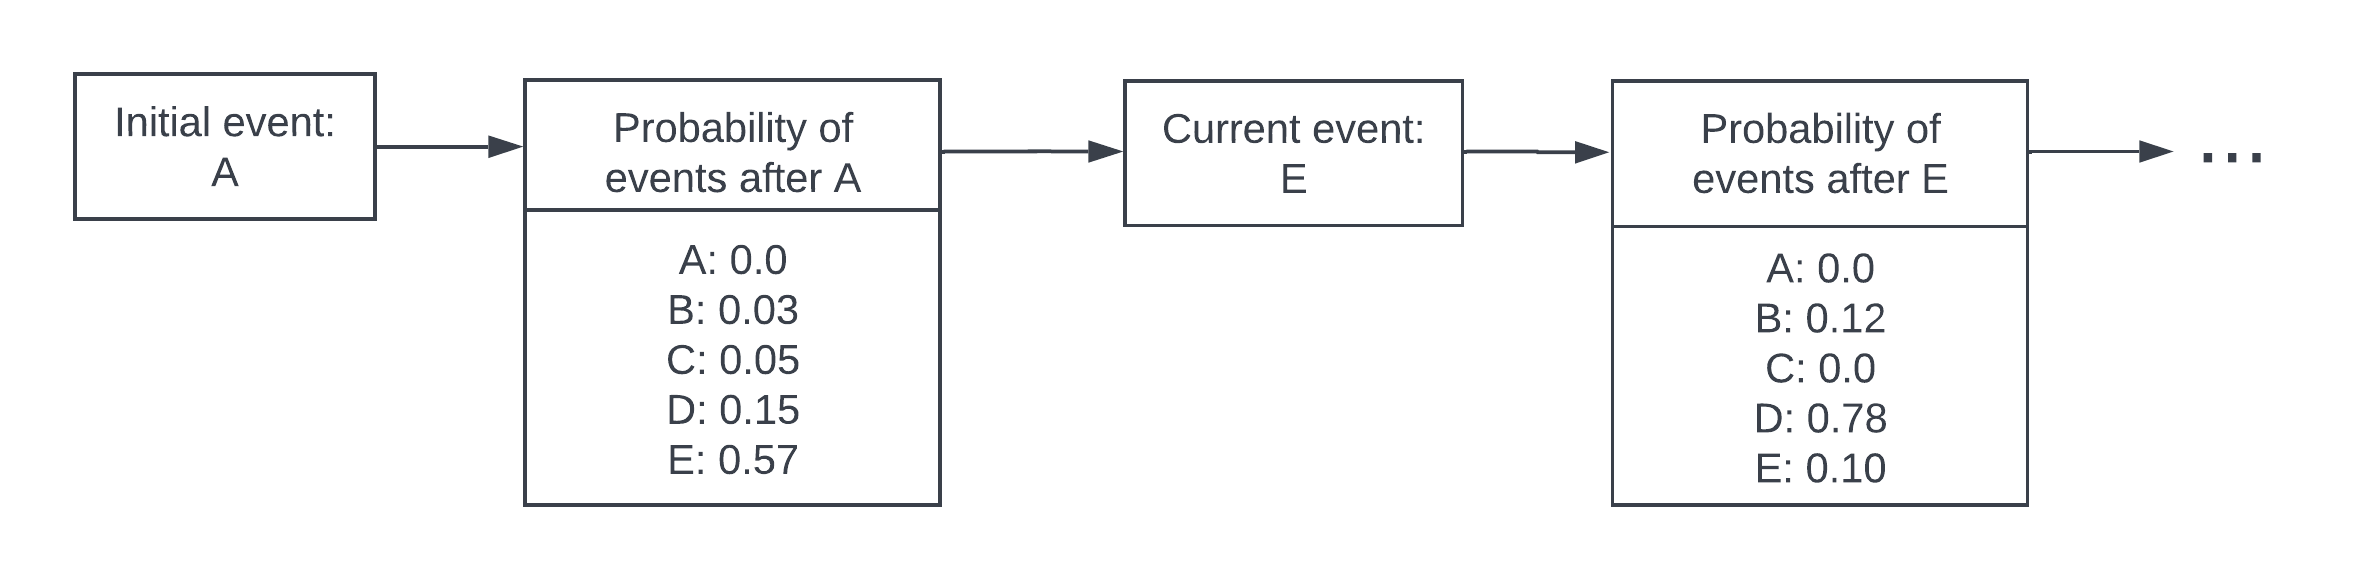
\includegraphics[width=0.9\textwidth]{assets/markov_chain_diagram.png}
        \caption{Visualization of a Markov Chain}
        \label{fig:markov_diagram}
    \end{center}
\end{figure}

It is worth noticing that Markov Chains are \textbf{not} Neural Networks, nor do they apply any learning algorithms. The process of calculating probabilities of next chords consists of going through a dataset once and counting frequencies of occurrences of chords regarding the previous chord. Despite being a simple model, the authors believe this approach gives a good baseline as to what can be expected from other, more sophisticated algorithms. The authors anticipate LSTMs and GANs to yield better results. \par


\section{Remarks and conclusions}

Three models provide a wide range of learning algorithms tackling the problem from different sides. One model treats music as images, the second one tries to infer semantics from sequences, and the last one is a simple statistical tool. This gives a good perspective into the problem of music generation and contrasts the performance of these approaches. While the underlying data format is the same (MIDI) for all models, the pre-processing varies for each prepared model and has to be carefully designed to fit the current needs. \par



\chapter{Project of application}


\section{Specification}

\subsection{Executive summary}

The application allows a user to upload his or her audio files in the MIDI format and train a selected model. Afterward, the user can generate a music sample created by the model trained on the provided input. All previously trained models are saved and available to be accessed at any time. The training progress is streamed and plotted in real time for all watching clients. The whole application is wrapped in a clean and simple Web user interface and accessible to everyone with an internet connection. \par

\subsection{Functional requirements}

To begin, a strict set of requirements must be defined. Most conditions are expressed as \textit{user stories} but a general list of requirements is also provided. A clear definition of a requirement is crucial as it ensures that the system is complete and cohesive. The system is split into three components, each with a separate responsibility: the \textit{server}, the \textit{client}, and the \textit{model}. \par

\subsubsection{User stories}

\newcommand{\AC}{\subitem AC. }

\textbf{\large Model:}

In this section, user stories regarding the \textit{model} component are presented.

\begin{enumerate}
    \item
          As a user, I want to be able to process MIDI files.
          \AC The \textit{model} component can read MIDI files and store them in a custom structure.

    \item
          As a user, I want to be able to train a model with a given input.
          \AC A function is exposed for each model which accepts input and trains the model.

    \item
          As an admin, I want to be able to track my model's performance.
          \AC Models save training progress.
          \AC Training progress can be accessed and processed further.

    \item
          As an admin, I want to be able to evaluate my model's performance.
          \AC Model can estimate its performance in a quantitative manner.

    \item
          As a user, I want to be able to save a trained model.
          \AC Model can be saved to a persistent medium.
          \AC A saved model is easily exportable to a different computer.

    \item
          As a user, I want to be able to load a saved model.
          \AC A model can be loaded from a persistent medium.
          \AC The model's performance is retained when loading the model.

    \item
          As a user, I want to be able to generate new music.
          \AC Models generate MIDI files based on a given seed.
\end{enumerate} \par

\textbf{\large Client and Server:}

In this section, user stories related to the \textit{client} and the \textit{server} components are presented. User stories describe the user perspective of interaction with the system; however, these entail some backend work as well.

\begin{enumerate}
    \item
          As a user, I want to be able to open a Web page containing an app interface.
          \AC A Web page displays the greeting interface.

    \item
          As a user, I want to be able to choose a target model.
          \AC The UI presents a selection field allowing one to choose a model.
          \AC Once the choice has been made a user can go to the next stage.

    \item
          As a user, I want to be able to pick either a pre-trained model or train one myself.
          \AC A user is presented with a choice between pre-trained and new models.
          \AC Once the choice has been made a user can go to the next stage.

    \item
          As a user, I want to be able to upload MIDI files if I choose to train a model myself.
          \AC The UI presents an option to choose a folder with MIDI files in it.
          \AC Files can be drag\&dropped for an upload.
          \AC Files are sent to the backend server.

    \item
          As a user, I want to be able to see training progress.
          \AC A live-updating chart shows the model training performance.

    \item
          As a user, I want to see when training has failed.
          \AC When training fails for assorted reasons, an error message is shown in the interface.

    \item
          As a user, I want to be able to generate music by providing a simple seed.
          \AC A user can provide a music seed to start the generation process.
          \AC Generated music is saved to a MIDI file on the user's computer.
\end{enumerate} \par

\subsubsection{Use-case descriptions}

A list of core functional requirements as use cases is presented in \tabref{requirements}. \par

% a phantom table to put caption before a table (\longtable doesn't support well \caption at the beginning of its body) - page numbering issue
\begin{table}[H]
    \caption{List of functional requirements of the application}
    \label{tab:requirements}
\end{table}
\addtocounter{table}{-1}

\begin{longtable}{ |S{0.12\textwidth}|S{0.15\textwidth}|S{0.25\textwidth}|S{0.37\textwidth}| }
    \hline
    \small Actor                             & \small Name                                        & \small Description                                                         & \small System response                                                                                                                                                                                                                        \\ \hline
    \endfirsthead
    \hline
    \small Actor                             & \small Name                                        & \small Description                                                         & \small System response                                                                                                                                                                                                                        \\ \hline
    \endhead
    \multicolumn{4}{|l|}{\textbf{Models}}                                                                                                                                                                                                                                                                                                                                                                                      \\ \hline
    \setlength{\baselineskip}{16pt}Developer & \setlength{\baselineskip}{16pt}Model training      & \setlength{\baselineskip}{16pt}Training a model with a given dataset       & \setlength{\baselineskip}{16pt}The module creates a previously defined model and trains it with progress saving.                                                                                                                              \\ \hline
    \setlength{\baselineskip}{16pt}Developer & \setlength{\baselineskip}{16pt}Model evaluation    & \setlength{\baselineskip}{16pt}Evaluating a model against given data       & \setlength{\baselineskip}{16pt}The module loads a previously trained model and evaluates its performance, after which the results are presented.                                                                                              \\ \hline
    \setlength{\baselineskip}{16pt}Developer & \setlength{\baselineskip}{16pt}Music generation    & \setlength{\baselineskip}{16pt}Generating music given a starting seed.     & \setlength{\baselineskip}{16pt}Model accepts a seed and generates a sequence. This sequence is saved to a MIDI file.                                                                                                                          \\ \hline
    \setlength{\baselineskip}{16pt}Developer & \setlength{\baselineskip}{16pt}MIDI parsing        & \setlength{\baselineskip}{16pt}Being able to read and write MIDI files.    & \setlength{\baselineskip}{16pt}System reads MIDI files and processes them to our needs. The system creates MIDI files from model outputs.                                                                                                     \\ \hline

    \multicolumn{4}{|l|}{\textbf{Server}}                                                                                                                                                                                                                                                                                                                                                                                      \\ \hline
    \setlength{\baselineskip}{16pt}Developer & \setlength{\baselineskip}{16pt}Model integration   & \setlength{\baselineskip}{16pt}Server and model components are integrated. & \setlength{\baselineskip}{16pt}Server component can query models for various tasks (i.e., training, evaluation, generation) and receives back responses.                                                                                      \\ \hline
    \setlength{\baselineskip}{16pt}Developer & \setlength{\baselineskip}{16pt}API                 & \setlength{\baselineskip}{16pt}Server exposes an API.                      & \setlength{\baselineskip}{16pt}Client receives responses from the server regarding queries and commands.                                                                                                                                      \\ \hline
    \setlength{\baselineskip}{16pt}Developer & \setlength{\baselineskip}{16pt}Live updates        & \setlength{\baselineskip}{16pt}Server exposes a bidirectional connection.  & \setlength{\baselineskip}{16pt}Client receives real-time information about a training progress.                                                                                                                                               \\ \hline
    \setlength{\baselineskip}{16pt}Developer & \setlength{\baselineskip}{16pt}File streaming      & \setlength{\baselineskip}{16pt}Streaming files from and to a client.       & \setlength{\baselineskip}{16pt}Client can download a file from the server. Server receives streamed files from the client.                                                                                                                    \\ \hline
    \multicolumn{4}{|l|}{\textbf{Client}}                                                                                                                                                                                                                                                                                                                                                                                      \\ \hline
    \setlength{\baselineskip}{16pt}User      & \setlength{\baselineskip}{16pt}Model configuration & \setlength{\baselineskip}{16pt}Configuration of target model               & \setlength{\baselineskip}{16pt}Buttons and switches are shown on the UI to allow to choose the model and training status (pre-trained or new).                                                                                                \\ \hline
    \setlength{\baselineskip}{16pt}User      & \setlength{\baselineskip}{16pt}File upload         & \setlength{\baselineskip}{16pt}Uploading local files to the server         & \setlength{\baselineskip}{16pt}Application accepts MIDI files to be uploaded. Files are sent to the backend server as the input dataset.                                                                                                      \\ \hline
    \setlength{\baselineskip}{16pt}User      & \setlength{\baselineskip}{16pt}Model training      & \setlength{\baselineskip}{16pt}Training a selected model                   & \setlength{\baselineskip}{16pt}Server communicates with the models to train them. Server streams the training progress back to the client. Client displays the training progress in a form of live-updating charts and/or standalone scalars. \\ \hline
    \setlength{\baselineskip}{16pt}User      & \setlength{\baselineskip}{16pt}Music generation    & \setlength{\baselineskip}{16pt}Using a model to generate music             & \setlength{\baselineskip}{16pt}Server communicates with the models to generate music sequences. Server sends a MIDI file back to the client. Client downloads the generated MIDI file.                                                        \\ \hline
\end{longtable}

\vfill
\subsubsection{Use case diagram}

Since most of the functionality is on the side of designing and creating models which are behind the scenes, the use case diagram can be neatly summarized to the main features as seen in \figref{use_case_diagram}. \par

\vfill
\newpage

\begin{figure}[t]
    \centering
    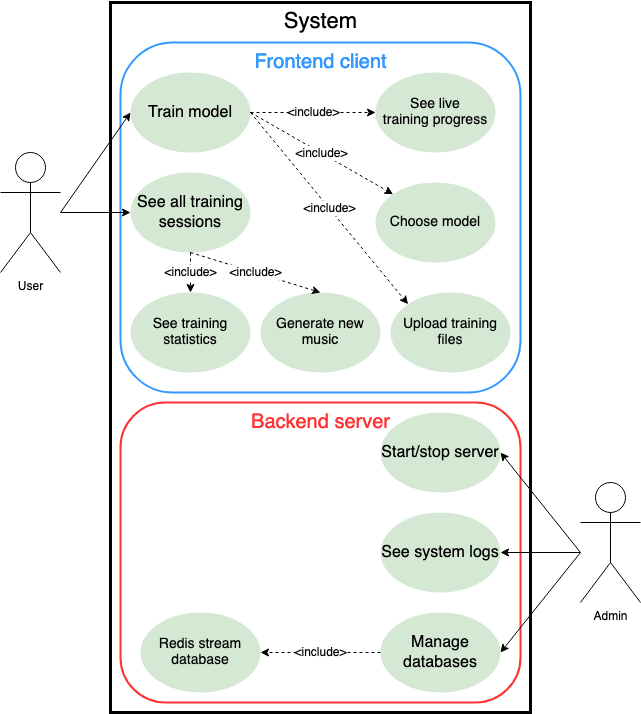
\includegraphics[width=0.7\textwidth]{use_case_diagram.png}
    \caption{Use case diagram for a user and an admin interacting with the system}
    \label{fig:use_case_diagram}
\end{figure} \par

\subsection{Non-functional requirements}

\tabref{URPS} shows non-functional requirements grouped into individual URPS categories. \par

% a phantom table to put caption before a table (\longtable does not support well \caption at the beginning of its body) - page numbering issue
\begin{table}[H]
    \caption{Non-functional requirements grouped by URPS categories}
    \label{tab:URPS}
\end{table}
\addtocounter{table}{-1}

\begin{longtable}{ |P{0.15\linewidth}|P{0.13\linewidth}|R{0.6\linewidth}| }
    \hline
    \small \setlength{\baselineskip}{12pt} Requirements area & \small \setlength{\baselineskip}{12pt} Requirement No. & \small \setlength{\baselineskip}{12pt} Description                                                                                                                                                       \\ \hline
    \endhead
    \multirow{6}{*}{Usability}                               & \setlength{\baselineskip}{16pt}1                       & \setlength{\baselineskip}{16pt}The application window must fit into a single screen of a standard size (at least 1920 x 1080px)                                                                          \\ \cline{2-3}
                                                             & \setlength{\baselineskip}{16pt}2                       & \setlength{\baselineskip}{16pt}The application must be clear and legible, with a font size no smaller than 10. All images and graphs displayed in the application must not be compressed in the runtime. \\ \cline{2-3}
                                                             & \setlength{\baselineskip}{16pt}3                       & \setlength{\baselineskip}{16pt}Application must be accessible and usable from all major platforms (i.e., Linux, macOS, Windows).                                                                         \\ \hline
    \setlength{\baselineskip}{16pt}Reliability               & \setlength{\baselineskip}{16pt}4                       & \setlength{\baselineskip}{16pt}The application must be available at least 99\% of the time, except for server service breaks.                                                                            \\ \hline
    \multirow{2.5}{*}{Performance}                           & \setlength{\baselineskip}{16pt}5                       & \setlength{\baselineskip}{16pt}The application should provide the exchange of information between a user and a server in no longer than 2 seconds.                                                       \\ \cline{2-3}
                                                             & \setlength{\baselineskip}{16pt}6                       & \setlength{\baselineskip}{16pt}While training a model, the application should be responsive to other actions.                                                                                            \\ \hline
    \multirow{2.5}{*}{Supportability}                        & \setlength{\baselineskip}{16pt}7                       & \setlength{\baselineskip}{16pt}The application must be backwards compatible with all of its components.                                                                                                  \\ \cline{2-3}
                                                             & \setlength{\baselineskip}{16pt}8                       & \setlength{\baselineskip}{16pt}In case of any exception, the application should provide detailed information to a user.                                                                                  \\ \hline
\end{longtable}


\section{Scope of work}

\tabref{scope_of_work} presents a division of the project into parts and tasks with their respective time necessary to finish each assignment. Seven main parts of the project were separated due to their subject. \par

% a phantom table to put caption before a table (\longtable does not support well \caption at the beginning of its body) - page numbering issue
\begin{table}[H]
    \caption{Main tasks within the project with time-to-complete}
    \label{tab:scope_of_work}
\end{table}
\addtocounter{table}{-1}

\begin{longtable}{ |S{0.11\linewidth}|S{0.59\linewidth}|P{0.18\linewidth}| }
    \hline
    \small Part No.                                                         & \small Task                                                                         & \small Duration (weeks) \\ \hline
    \endhead
    \multicolumn{2}{|l|}{\textbf{1. Project preparation}}                   &                                                                                                               \\ \hline
    1.1                                                                     & \setlength{\baselineskip}{16pt}Research and study on the thesis' topic              & 5                       \\ \hline
    1.2                                                                     & \setlength{\baselineskip}{16pt}Research and study on available algorithms and tools & 5                       \\ \hline
    1.3                                                                     & \setlength{\baselineskip}{16pt}Choice of AI algorithms and the technology stack     & 1                       \\ \hline
    \multicolumn{2}{|l|}{\textbf{2. Data management}}                       &                                                                                                               \\ \hline
    2.1                                                                     & \setlength{\baselineskip}{16pt}Research of available datasets                       & 2                       \\ \hline
    2.2                                                                     & \setlength{\baselineskip}{16pt}Choice of datasets to be included and accessing them & 1                       \\ \hline
    2.3                                                                     & \setlength{\baselineskip}{16pt}Implementation of the MIDI transcription module      & 5                       \\ \hline
    \multicolumn{2}{|l|}{\textbf{3. GAN model development}}                 &                                                                                                               \\ \hline
    3.1                                                                     & \setlength{\baselineskip}{16pt}Model implementation                                 & 3                       \\ \hline
    3.2                                                                     & \setlength{\baselineskip}{16pt}Model evaluation                                     & 1                       \\ \hline
    3.3                                                                     & \setlength{\baselineskip}{16pt}Model testing and tuning                             & 2                       \\ \hline
    \multicolumn{2}{|l|}{\textbf{4. Markov chain model development}}        &                                                                                                               \\ \hline
    4.1                                                                     & \setlength{\baselineskip}{16pt}Model implementation                                 & 1                       \\ \hline
    4.2                                                                     & \setlength{\baselineskip}{16pt}Model evaluation                                     & 1                       \\ \hline
    4.3                                                                     & \setlength{\baselineskip}{16pt}Model testing and tuning                             & 1                       \\ \hline
    \multicolumn{2}{|l|}{\textbf{5. LSTM model development}}                &                                                                                                               \\ \hline
    5.1                                                                     & \setlength{\baselineskip}{16pt}Model implementation                                 & 3                       \\ \hline
    5.2                                                                     & \setlength{\baselineskip}{16pt}Model evaluation                                     & 1                       \\ \hline
    5.3                                                                     & \setlength{\baselineskip}{16pt}Model testing and tuning                             & 2                       \\ \hline
    \multicolumn{2}{|l|}{\textbf{6. Client-server application development}} &                                                                                                               \\ \hline
    6.1                                                                     & \setlength{\baselineskip}{16pt}Web API server setup                                 & 3                       \\ \hline
    6.2                                                                     & \setlength{\baselineskip}{16pt}Databases setup                                      & 2                       \\ \hline
    6.3                                                                     & \setlength{\baselineskip}{16pt}Implementation of the training manager               & 3                       \\ \hline
    6.4                                                                     & \setlength{\baselineskip}{16pt}Graphical user interface design and implementation   & 3                       \\ \hline
    6.5                                                                     & \setlength{\baselineskip}{16pt}Application integration with the AI models           & 2                       \\ \hline
    \multicolumn{2}{|l|}{\textbf{7. Testing}}                               &                                                                                                               \\ \hline
    7.1                                                                     & \setlength{\baselineskip}{16pt}Unit testing                                         & 2                       \\ \hline
    7.2                                                                     & \setlength{\baselineskip}{16pt}Integration testing                                  & 1                       \\ \hline
    7.3                                                                     & \setlength{\baselineskip}{16pt}System testing                                       & 1                       \\ \hline
    7.4                                                                     & \setlength{\baselineskip}{16pt}Efficiency and quality comparison of the AI models   & 1                       \\ \hline
    7.5                                                                     & \setlength{\baselineskip}{16pt}Final corrections and a system review                & 1                       \\ \hline
\end{longtable}

\vfill
\section{Risk analysis}
A risk analysis of the project was done using the 'SWOT' methodology. The result is presented in Table \ref{tab:SWOT}. \par

\vfill
\section{System architecture}

The application consists of three modules. They are designed so that replacing any module does not affect other ones. \par

\vfill
\newpage

\begin{table}[H]
    \centering
    \caption{Risk analysis of the project divided into SWOT categories} \vskip16pt
    \label{tab:SWOT}
    \begin{tabular}{ |P{0.14\linewidth}|P{0.39\linewidth}|P{0.39\linewidth}| }
        \hline
        \textbf{SWOT}                                                                                                                                                                        & \setlength{\baselineskip}{14pt} HELPFUL                & \setlength{\baselineskip}{14pt} HARMFUL             \\
        \hline
        \setlength{\baselineskip}{14pt}                                                                                                                                                      &                                                        &                                                     \\
        \setlength{\baselineskip}{14pt}INTERNAL                                                                                                                                              & \setlength{\baselineskip}{14pt}\textbf{Strengths:}     & \setlength{\baselineskip}{14pt}\textbf{Weaknesses:} \\
        \setlength{\baselineskip}{14pt}                                                                                                                                                      &
        \setlength{\baselineskip}{14pt}\begin{enumerate}
                                           \setlength{\baselineskip}{14pt}    \item One of the authors has experience in developing music-generating AI systems,
                                                 \setlength{\baselineskip}{14pt}    \item Possibility of consultation of solution design with people experienced in the field of music generation and AI (e.g., thesis Supervisor),
                                                 \setlength{\baselineskip}{14pt}    \item Extensive coverage of capabilities of used tools both in documentations and on the Internet,
                                                 \setlength{\baselineskip}{14pt}    \item Multiple sets with MIDI files available in the free domain,
                                                 \setlength{\baselineskip}{14pt}    \item Good communication skills and motivation of all authors.
                                                 \setlength{\baselineskip}{14pt}\end{enumerate}   &
        \setlength{\baselineskip}{14pt}\begin{enumerate}
                                           \setlength{\baselineskip}{14pt}    \item A short period dedicated to developing core functions, while some learning algorithms may require a significant amount of time to perform their tasks,
                                                 \setlength{\baselineskip}{14pt}    \item Quality of results cannot be predicted straightforwardly,
                                                 \setlength{\baselineskip}{14pt}    \item Impossibility of generating a MIDI set by one's own -- the project depends on works by external authors,
                                                 \setlength{\baselineskip}{14pt}    \item Large size, quality, and feature differences among MIDI sets.
                                                 \setlength{\baselineskip}{14pt}\end{enumerate}                                                                       \\
        \hline
        \setlength{\baselineskip}{14pt}                                                                                                                                                      &                                                        &                                                     \\
        \setlength{\baselineskip}{14pt}EXTERNAL                                                                                                                                              & \setlength{\baselineskip}{14pt}\textbf{Opportunities:} & \setlength{\baselineskip}{14pt}\textbf{Threats:}    \\
        \setlength{\baselineskip}{14pt}                                                                                                                                                      &
        \setlength{\baselineskip}{14pt}\begin{enumerate}
                                           \setlength{\baselineskip}{14pt}    \item A raise of competence in the field of Artificial Intelligence,
                                                 \setlength{\baselineskip}{14pt}    \item Possibility of further development of the project (e.g., as a master's thesis),
                                                 \setlength{\baselineskip}{14pt}    \item Possibility of publishing the project on the Internet and gaining users (similarly to other AI projects, e.g., DALL-E and its derivatives).
                                                 \setlength{\baselineskip}{14pt}\end{enumerate} &
        \setlength{\baselineskip}{14pt}\begin{enumerate}
                                           \setlength{\baselineskip}{14pt}    \item Simultaneous completion of multiple projects throughout the final semester,
                                                 \setlength{\baselineskip}{14pt}    \item Some functionalities regarding learning algorithms may be prone to fail or take too long to complete due to unsatisfactory (substandard) parameters of a user's PC,
                                                 \setlength{\baselineskip}{14pt}    \item Consecutive development of the solution may happen in different periods than defined in the university's curriculum due to the need to focus on AI algorithms.
                                                 \setlength{\baselineskip}{14pt}\end{enumerate}                                                          \\
        \hline
    \end{tabular}
\end{table}

\subsection{Models}

This module consists of the definition and implementation of models. All models share a common interface so their implementation details are hidden. This is a requirement for ease of integration with the backend module. All concerns regarding the processing of MIDI files are addressed here. Each model has its specific preferences and thus needs to decide how a raw MIDI file should be prepared. \par
While training, all models must report their progress in any preferred metric in real time. Once all training is done, each model should be able to generate a new music sample in the MIDI format. Finally, each model must be able to serialize and deserialize itself, so that it can be released from memory and persisted to a disk. With all that in mind, \figref{musicmodel_class_diagram} depicts the class diagram of the common abstract class extended by all the models. These classes will define a certain model architecture. They will inherit methods and properties from the \textit{MusicModel} class so that we can assure they all are compatible with the API. This is not restricted to the selected three models: one could implement this interface for any new model, and it would fit into the system seamlessly. \par

\begin{figure}[H]
    \centering
    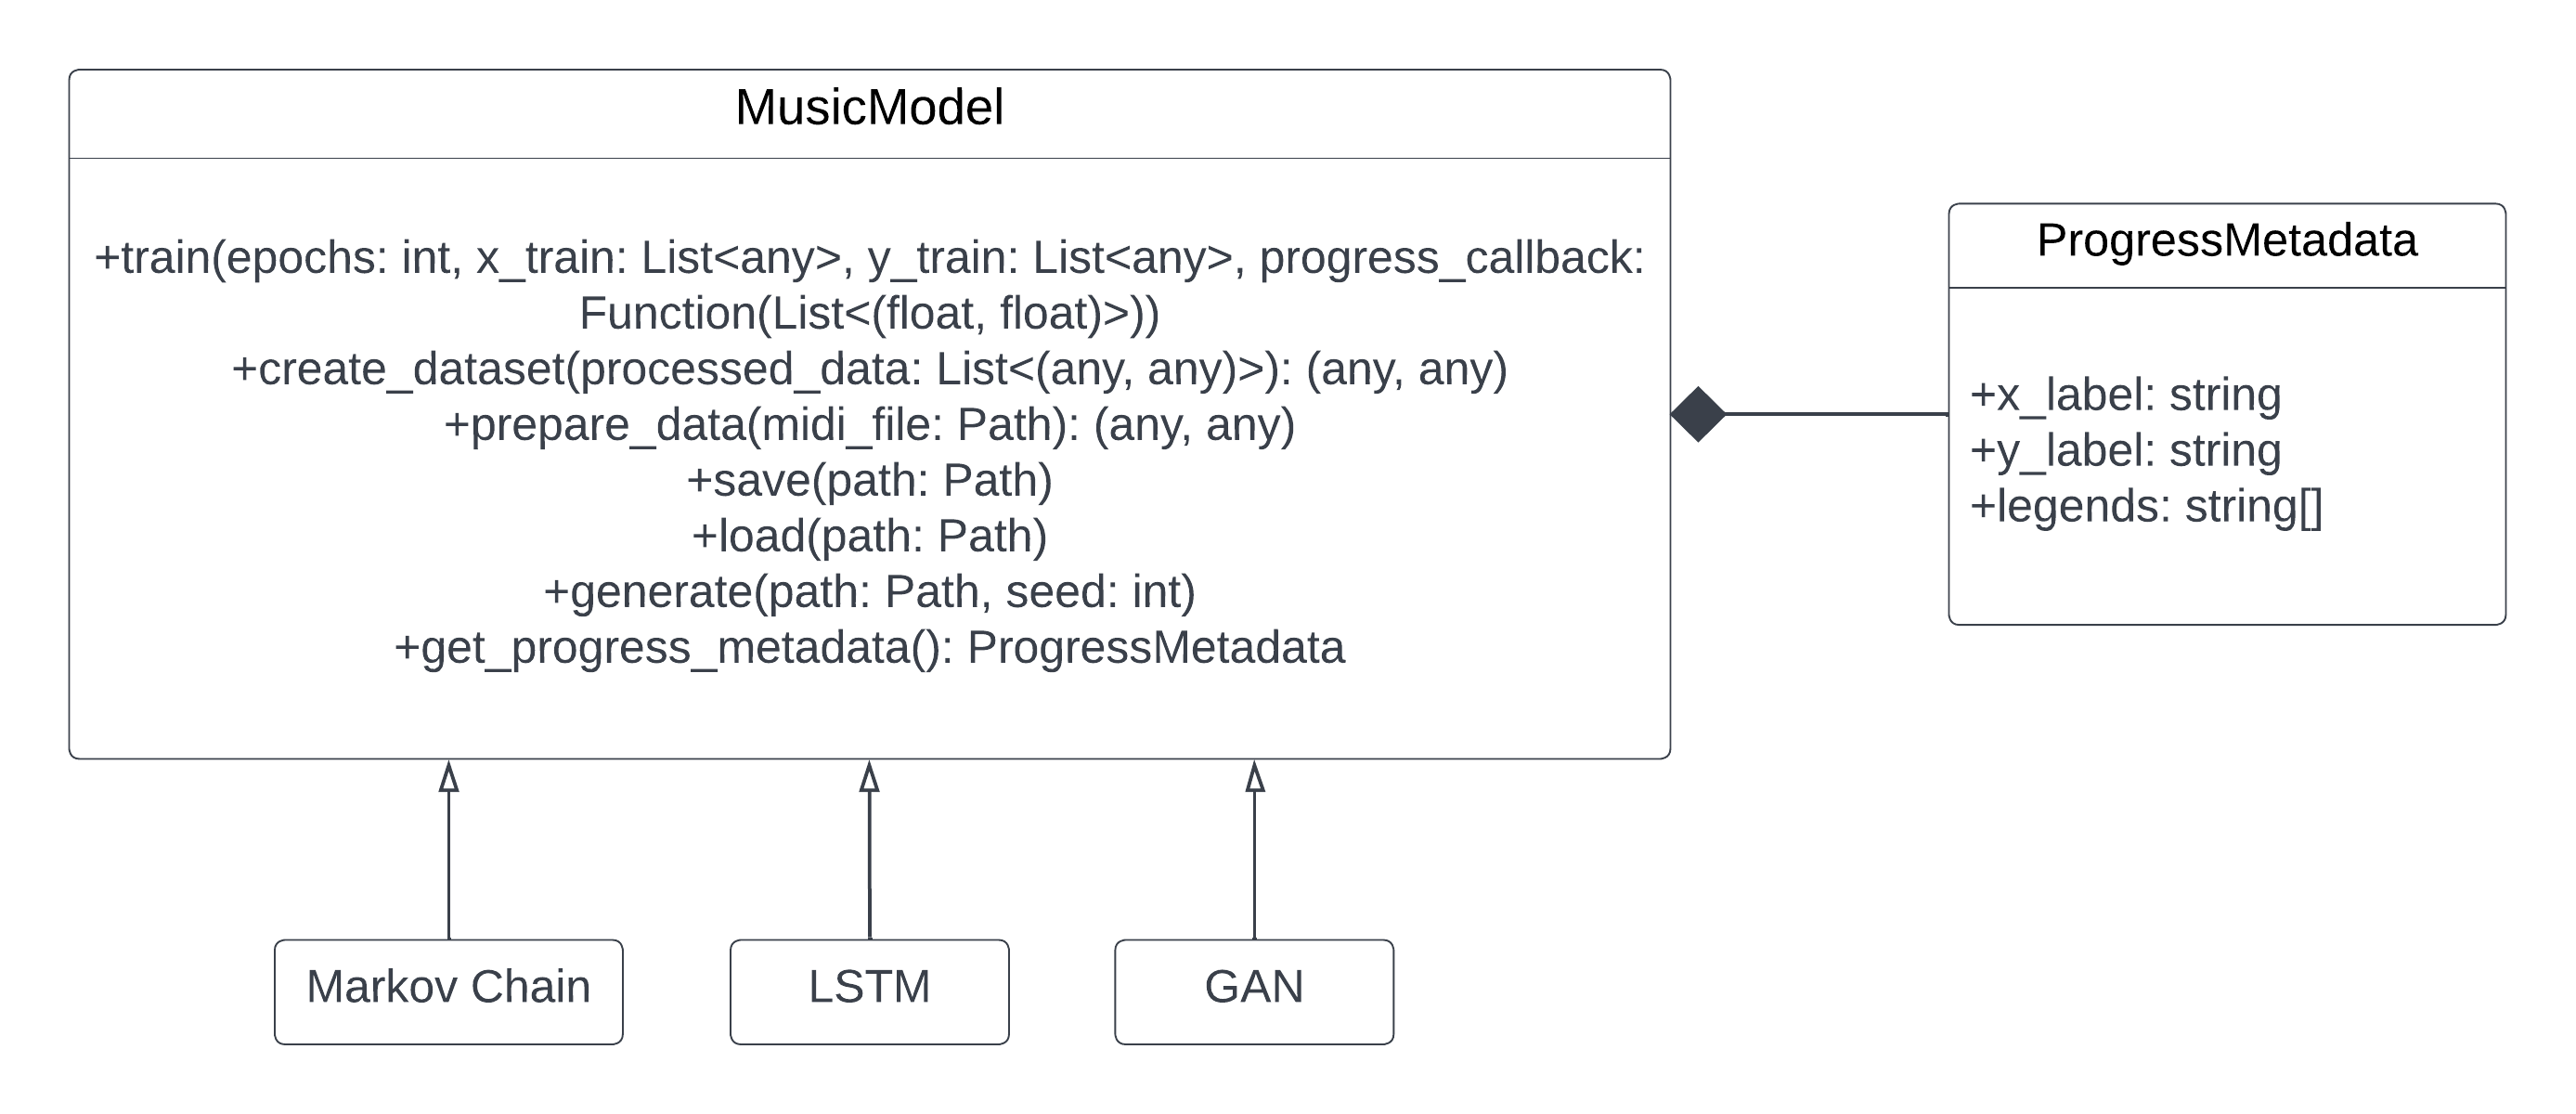
\includegraphics[width=0.9\textwidth]{class_models.png}
    \caption{Class diagram of the MusicModel abstract class}
    \label{fig:musicmodel_class_diagram}
\end{figure}

This common class contains all methods needed for the model-backend integration. First, a model instance is created, and the dataset is prepared with \texttt{prepare\_data} which is called with a path to MIDI files. Then the processed files are turned into a dataset with \texttt{create\_dataset}, this dataset is then fed into \texttt{train} together with an epoch count and a callback function for progress reporting. Metadata about progress information is gathered from \texttt{get\_progress\_metadata}. This allows the system to plot training values. \par

\subsection{Backend server}

The role of a backend server is to be a bridge between users and models. Other than connecting with models, the backend is responsible for managing databases and persisting user data. To accommodate these needs, a few structures are needed as seen in \figref{backend_class_diagram}. Two main repositories are distinguished. The first one is \texttt{TrainingProgressRepository} which manages live training progress data of models. This utilizes a cross-process publish-subscribe pattern where one can publish events of training progress as well as listen to a specific stream. Training progress is expressed in a very generic fashion to allow models to express their progress for their special needs while retaining the flexibility. This format is a simple list of pairs of floating point numbers. The $i$-th element represents the most recent point on the $i$-th chart line. Training can fail for various reasons, hence why the repository also allows terminating publish-subscribe streams and complete with an error using the \texttt{publish\_error} method. \par
As opposed to the previous repository, the \texttt{TrainingSessionsRepository} class manages persistent data instead of ephemeral one. Here, the creation of sessions happens together with all data accompanied by it. This includes model information, training data, or training errors. Saved information can also be retrieved through various methods. The underlying storage is a database which is a simple collection of two tables with a one-to-many relation between a training session and its training files (\figref{db_class_diagram}). \par
Finally, the \texttt{TrainingManager} uses previously mentioned repositories to manage the process of training models and propagating training information to appropriate sources. It ensures the system is left in a coherent state. \par

\begin{figure}
    \centering
    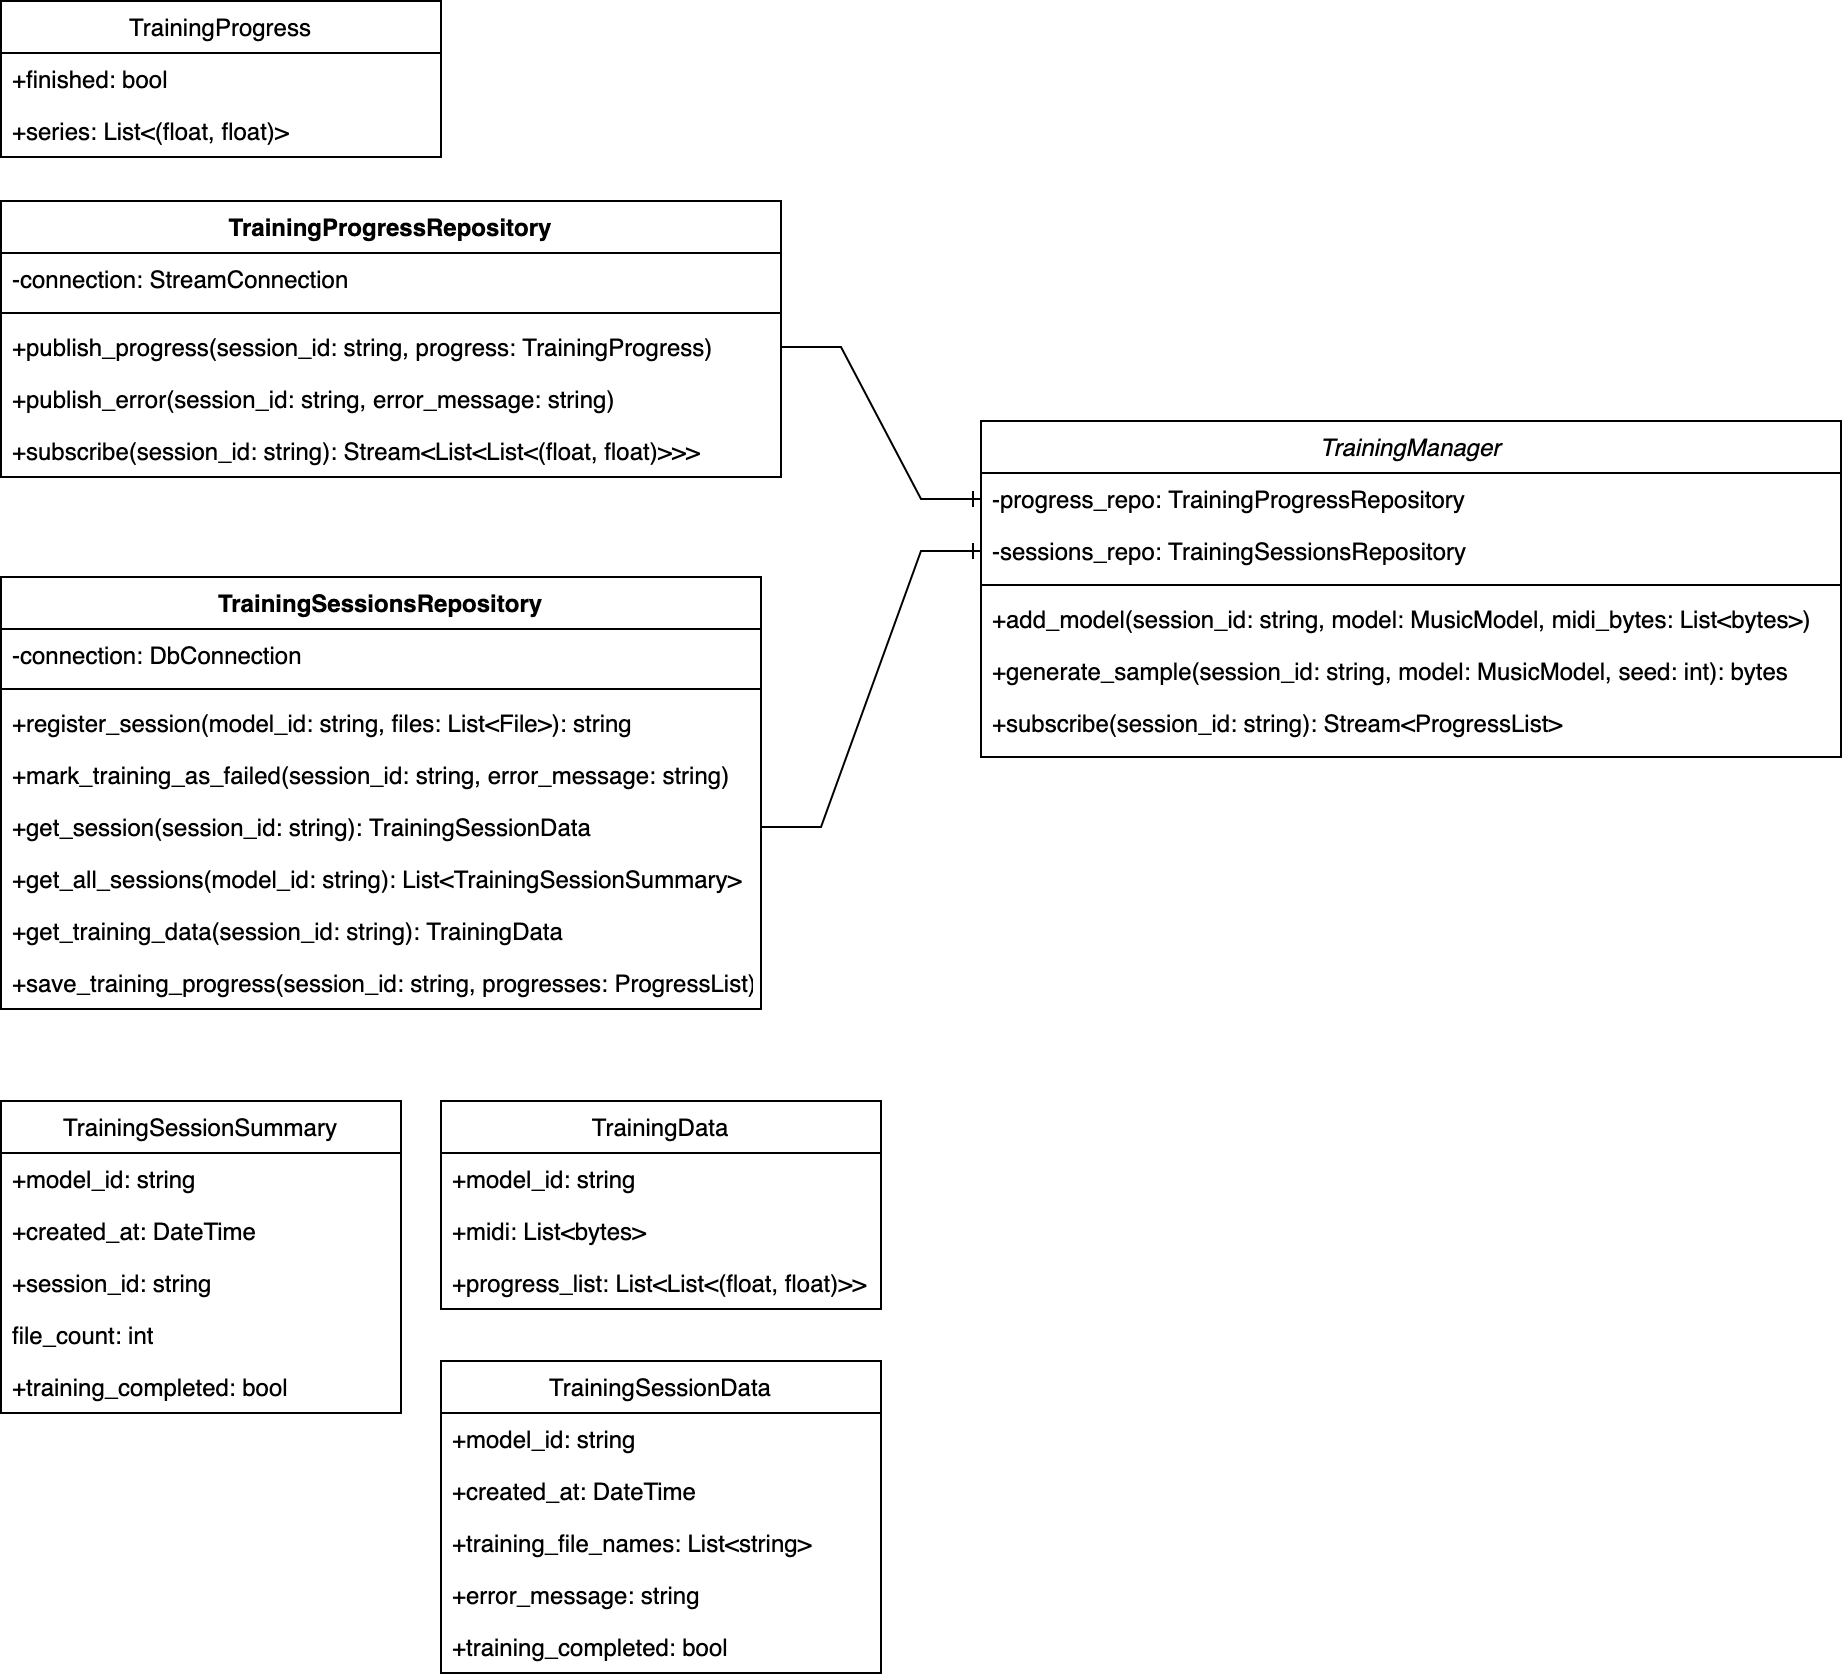
\includegraphics[width=0.9\textwidth]{backend_class.png}
    \caption{Class diagrams of the backend module}
    \label{fig:backend_class_diagram}
\end{figure}

\begin{figure}
    \centering
    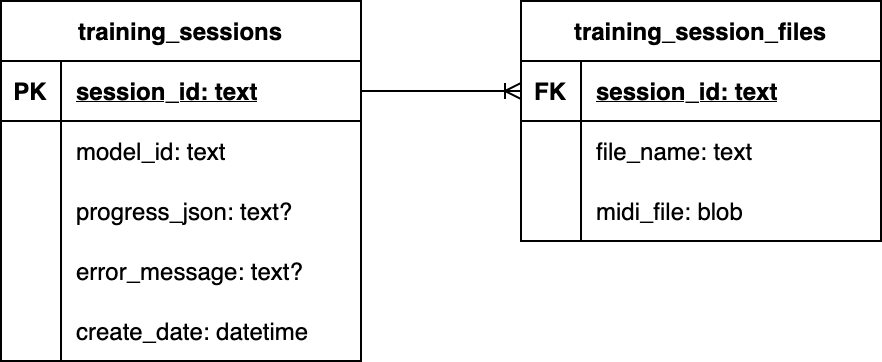
\includegraphics[width=0.7\textwidth]{database_class.png}
    \caption{Class diagrams of the database tables}
    \label{fig:db_class_diagram}
\end{figure}

The backend of the application consists mainly of API endpoint code which allows for communication between a chosen model and a client. It is described in more detail in Section \ref{sec:communication} and the OpenAPI specification, attached separately. \par

\subsection{Frontend}

The frontend module provides the GUI which allows its users to control the application. It must be intuitive and responsive. Additionally, its usage should not require any knowledge about the underlying models. To ensure accessibility, the frontend is a Web application with a simple interface allowing one to train and use various models. This module reflects the API provided by the backend module. The interface is also resilient to errors by handling all failures and displaying them to end users. \par


\section{Communication} \label{sec:communication}

The three modules -- the models, the backend, and the frontend -- have a bidirectional linear communication flow, that is, each component interacts with a single another one. Thus the communication schemes are differentiated further in this chapter. \par

\subsection{Models \texorpdfstring{$\leftrightarrow$}{<->} Backend}

Since the backend and the models are just two different Python packages, the communication between them happens through direct function calls. No special protocol is required here other than the assumption of interoperability between packages which is conserved because these are written using the same versions of Python and its dependencies. \par

\subsection{Backend \texorpdfstring{$\leftrightarrow$}{<->} Frontend}

Two types of backend-frontend communication can be distinguished: request-response and real-time. In both cases, the communication can be performed in either unsecured or secure contexts. It is important in local development where the setup of a secure context is mostly a needless burden. The communication protocols are respectively HTTP/HTTPS and WS/WSS. \par

\subsubsection{Request-Response}

For a single request-single response communication, the HTTP protocol is used as a widely accepted standard for the Web. The backend supports both HTTP/1.1 and HTTP/2, allowing browser clients to choose their preferred method of communication. There is also a simple way to introduce HTTP/3 support but it is not implemented in this project. For a meta-protocol, REST is a popular choice and thus is used with a small adjustment to adhere to the core CQRS \cite{CQRS} principle: queries should be idempotent and fetch some data (represented as HTTP's \texttt{GET} method), and commands should modify some data but not return any (represented as HTTP's \texttt{POST} method). This simple modification allows for easy testing and maintainability. \par
In a separate attachment, one can find the OpenAPI specification of the application's API. \par

\subsubsection{Real-Time}

Some aspects require implementing real-time communication; that is, data can flow both ways without a predictable end of a connection. For instance, when a model is being trained, the backend continuously pushes data regarding the current training status to clients listening to this training session. In that case, it is unreasonable to expect the client to poll for the newest training status all of the time. WebSockets fit this task perfectly. They allow for connections to be created where both ends can push messages without any additional trigger. \par

\subsection{Internal backend} \label{sec:comm_backend}

The backend requires internal communication with outside services not developed by authors. These are used by database connections. One connection uses SQLite driver to communicate with SQLite databases. Another one uses the Redis protocol for connecting to Redis cache servers, used for streaming training progress to all server instances. \par
The whole communication can be summarized in a single figure (\figref{communication_diagram}). \par

\begin{figure}[H]
    \centering
    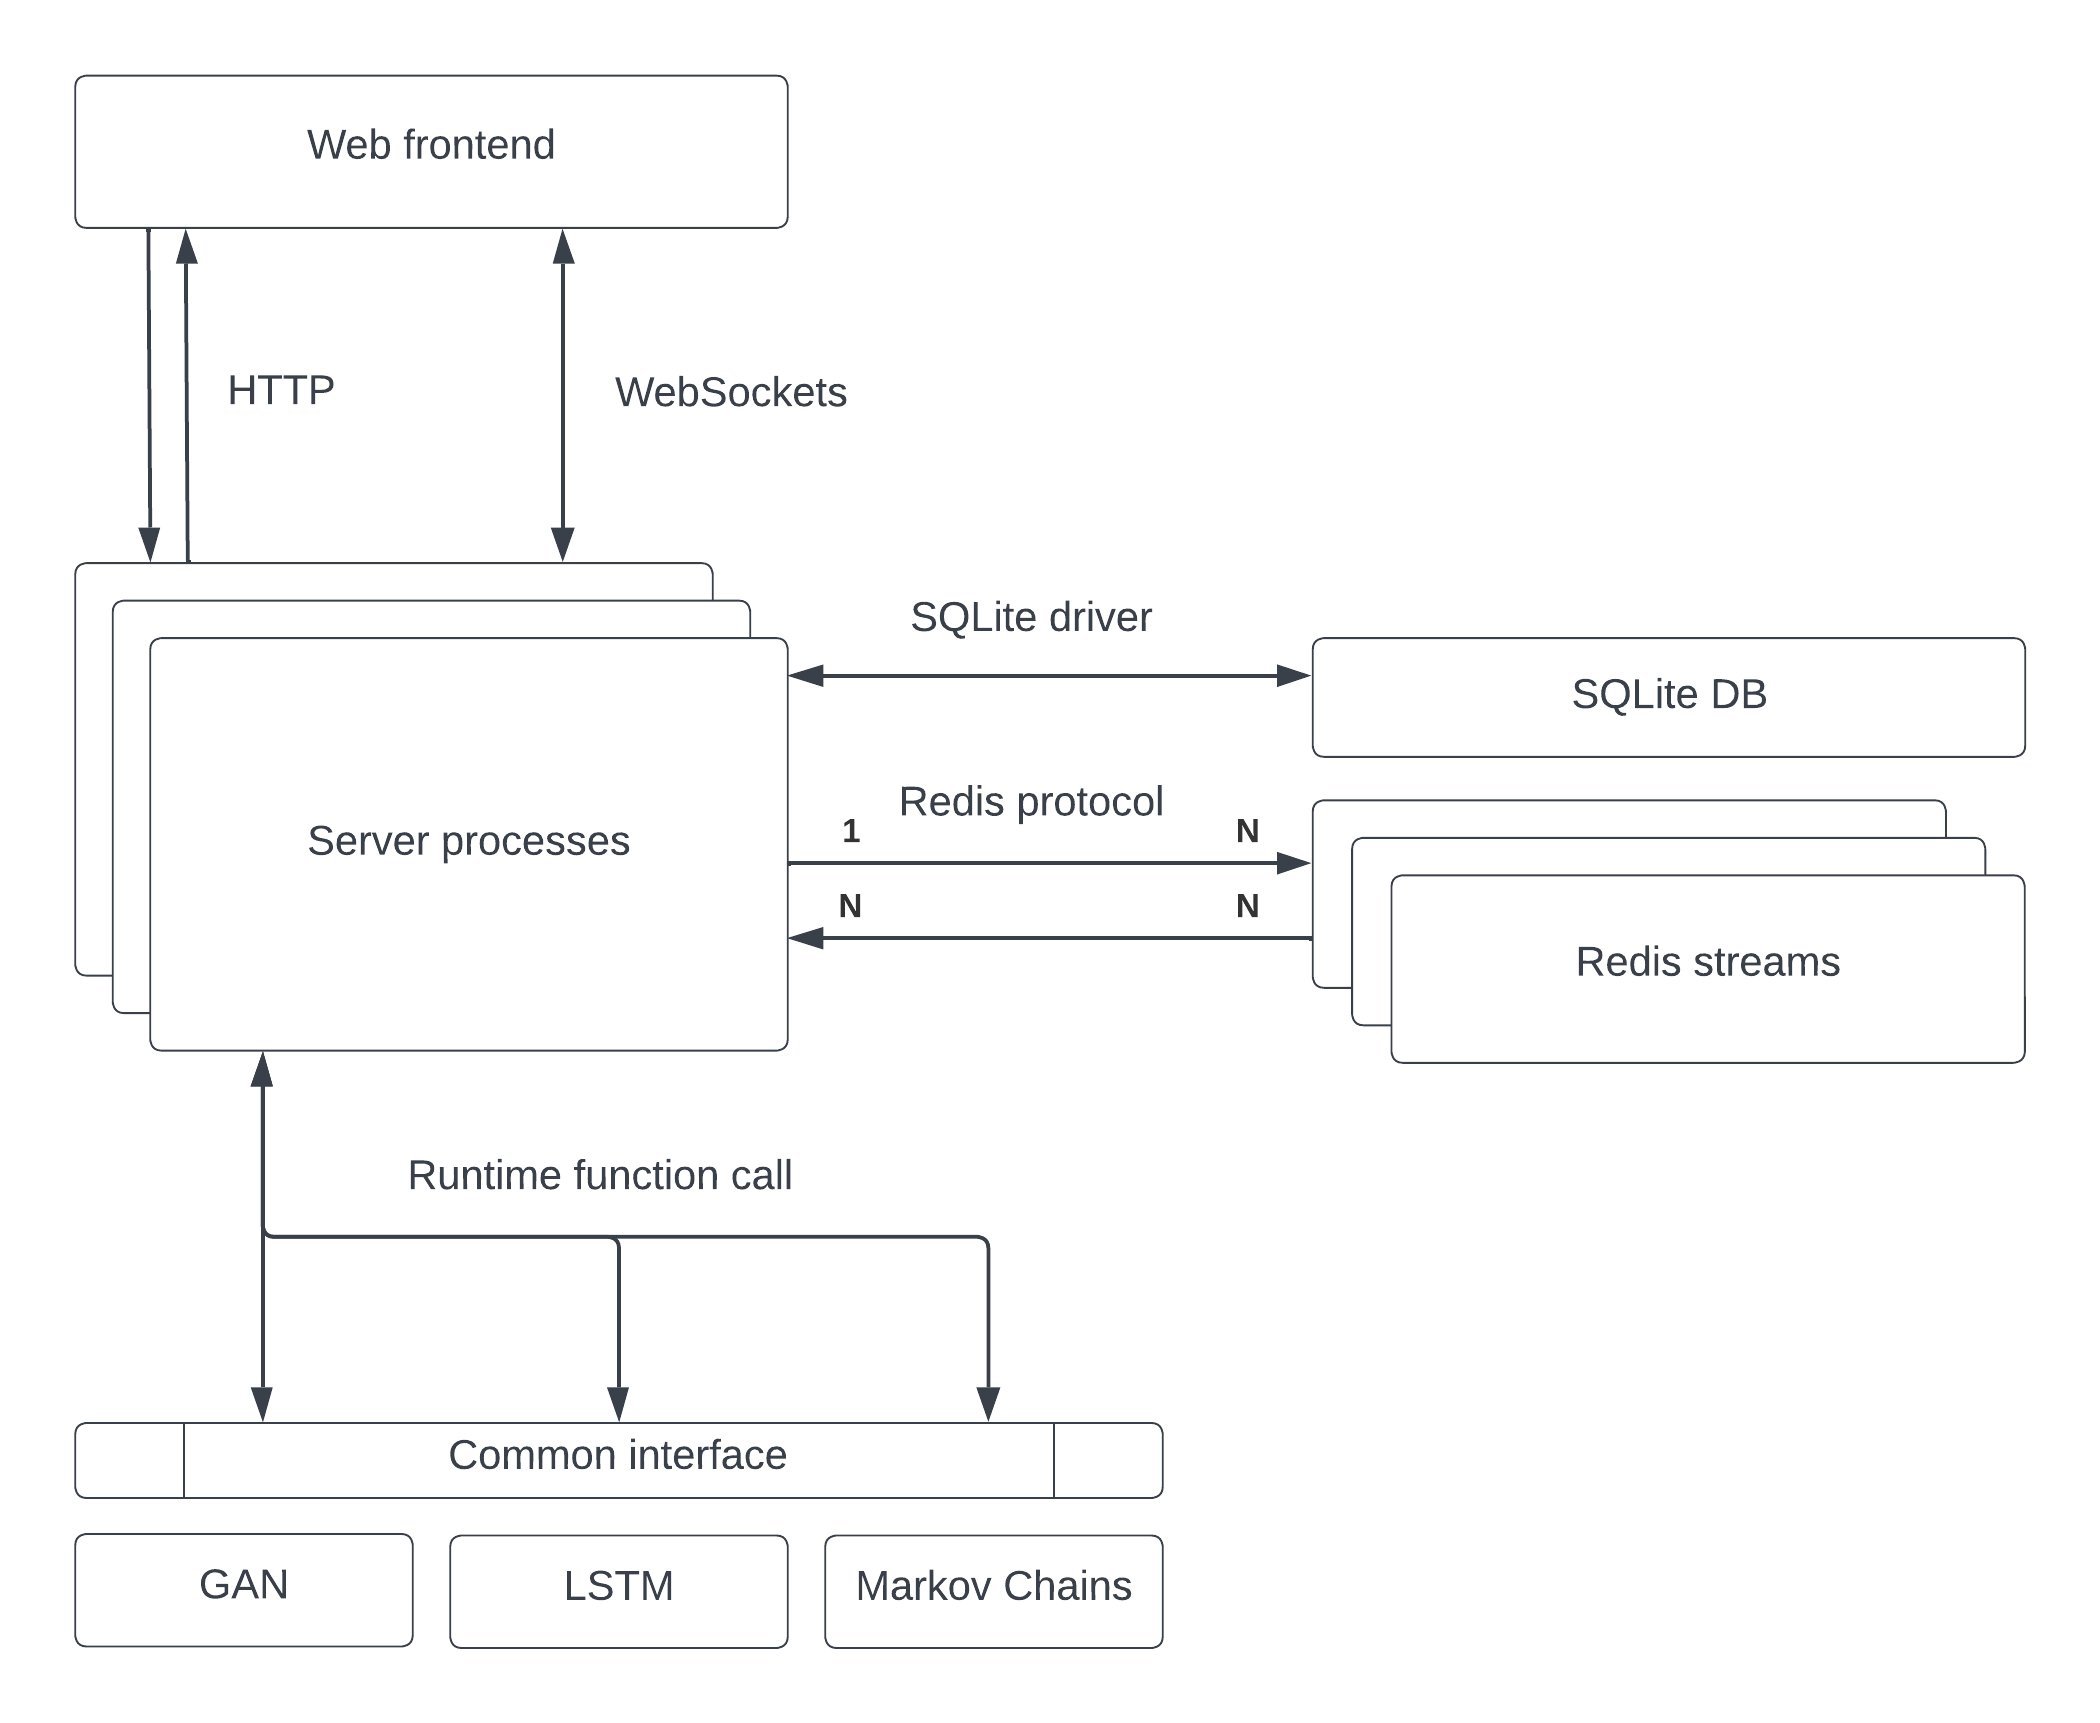
\includegraphics[width=0.8\textwidth]{assets/communication_diagram.png}
    \caption{Communication diagram for all modules in the application. Arrowheads represent directions of communication}
    \label{fig:communication_diagram}
\end{figure}

\section{GUI vision}

\begin{figure}[!t]
    \centering
    
\includegraphics[width=0.7\linewidth]{gui_dark.png}
    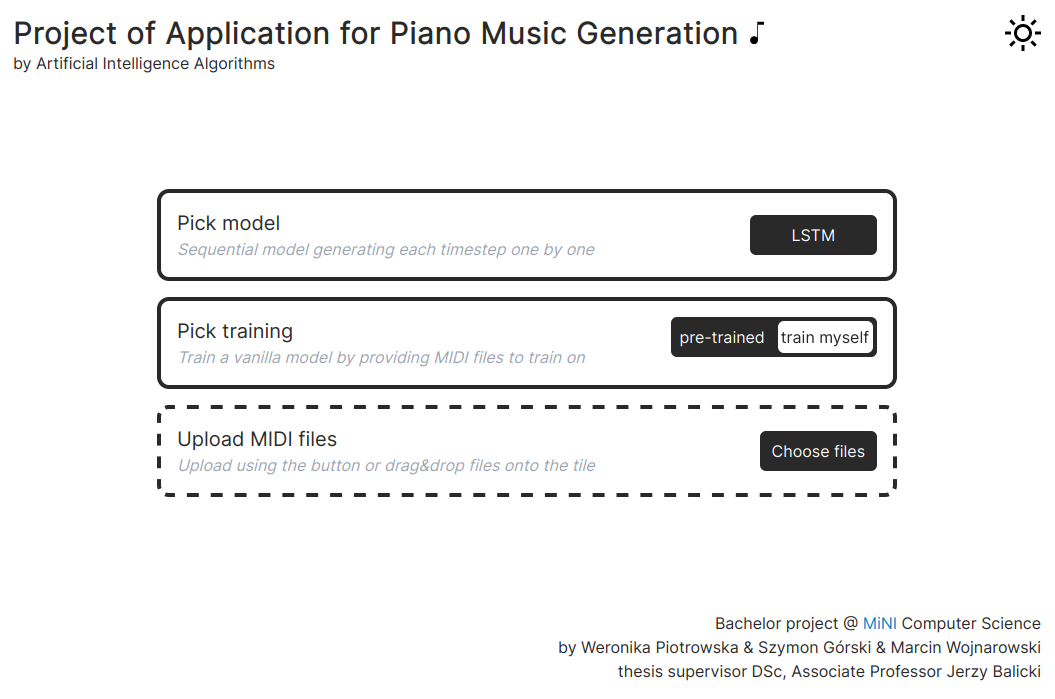
\includegraphics[width=0.7\linewidth]{gui_light.png}
    \caption{The home page of the user interface, in dark and light theme, respectively}
    \label{fig:gui_home}
\end{figure}

Projects which implement deeply technical subjects often have unpleasant and convoluted user interfaces. Little attention is given to the look and experience, yet this is also a part of engineering. It is shown in this section that creating a usable and intuitive user interface requires little effort yet greatly affects users' impressions of the software. \par
The UI focuses on simplicity and ease of use. None of the existing UI frameworks nor design systems suited the needs of the authors, therefore a custom implementation in a two-tone design language was created from scratch. The composition is minimalistic and the navigation has a linear flow which creates a self-explainable user experience. \par
The product follows accessibility principles such as semantic elements, descriptive alt labels, or keyboard navigation. The interface supports two themes (see \figref{gui_home}), dark and light. Both provide a high contrast which improves accessibility. \par
To guide the user through the configuration options, elements requiring action from a user are marked with a dashed border (see \figref{gui_action}) but once completed are turned into a solid border. This gives a clear indication of what action is expected next and how one can complete it. \par

\begin{figure}[t]
    \centering
    
\includegraphics[width=0.6\linewidth]{gui_action_todo.png}
    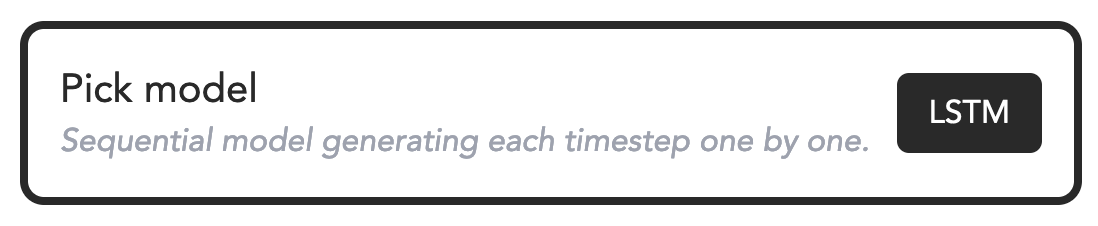
\includegraphics[width=0.6\linewidth]{gui_action_done.png}
    \caption{An element of the GUI requiring user's attention before and after being completed, respectively}
    \label{fig:gui_action}
\end{figure}

\begin{figure}[t]
    \centering
    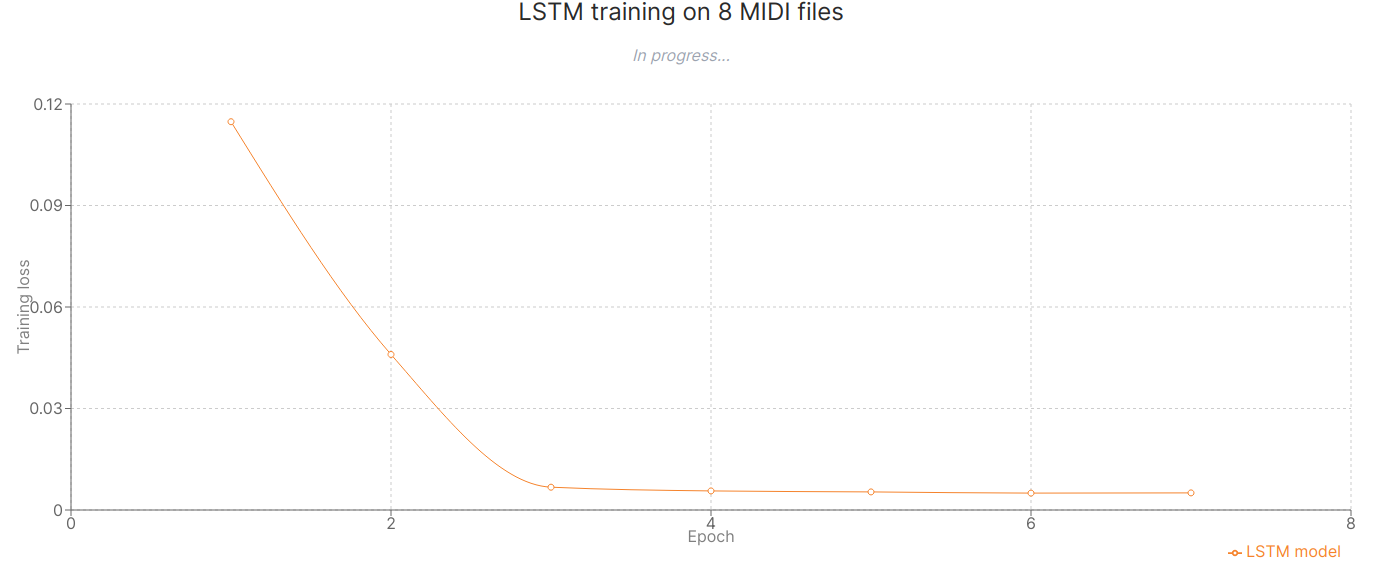
\includegraphics[width=0.98\linewidth]{gui_training_chart.png}
    \caption{Example training plot for the LSTM model}
    \label{fig:gui_chart}
\end{figure}

There are two paths a user can go through: training a model from scratch or picking a model that was trained previously. \par

\subsection{Training models}

Once the \textit{train myself} option is chosen, a user is asked to upload MIDI files. Once done, a training session is created, and the user is navigated to a dedicated screen. During the training, the UI updates itself in real time with training results. These values are represented as a plot on a chart alongside additional relevant information (see \figref{gui_chart}). \par
When training is done, a user is presented with the possibility of providing a seed to generate a new, larger sample of music. To do so, input is accepted from an on-screen piano keyboard presented in \figref{gui_record_seed}. After the seed is recorded, a new sample is generated by the underlying model and sent to the client as a MIDI file. \par

\begin{figure}[t]
    \centering
    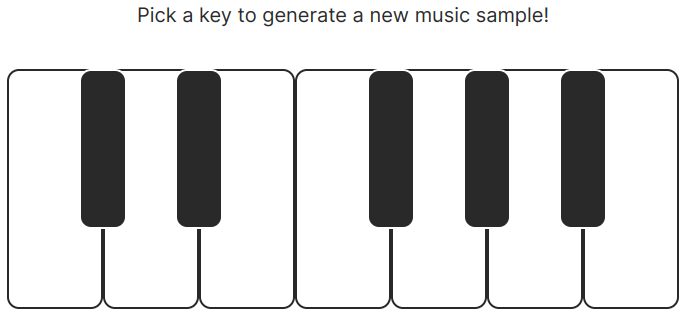
\includegraphics[width=0.6\linewidth]{gui_record_seed.png}
    \caption{An on-screen piano keyboard for recording a generation seed}
    \label{fig:gui_record_seed}
\end{figure}

In case of any errors during training, the process is stopped and the error is displayed to the user. \par

\subsection{Seeing previous models}

All trained models (whether successful or not) can be previewed and those that have completed training can be used for music generation. It is done by choosing the \textit{pre-trained} option and then choosing a preferred model instance (as presented in \figref{gui_choose_existing_model}). This leads to the same screen as any new training, so all statistics can still be viewed along with a generation of new music samples. \par

\begin{figure}[t]
    \centering
    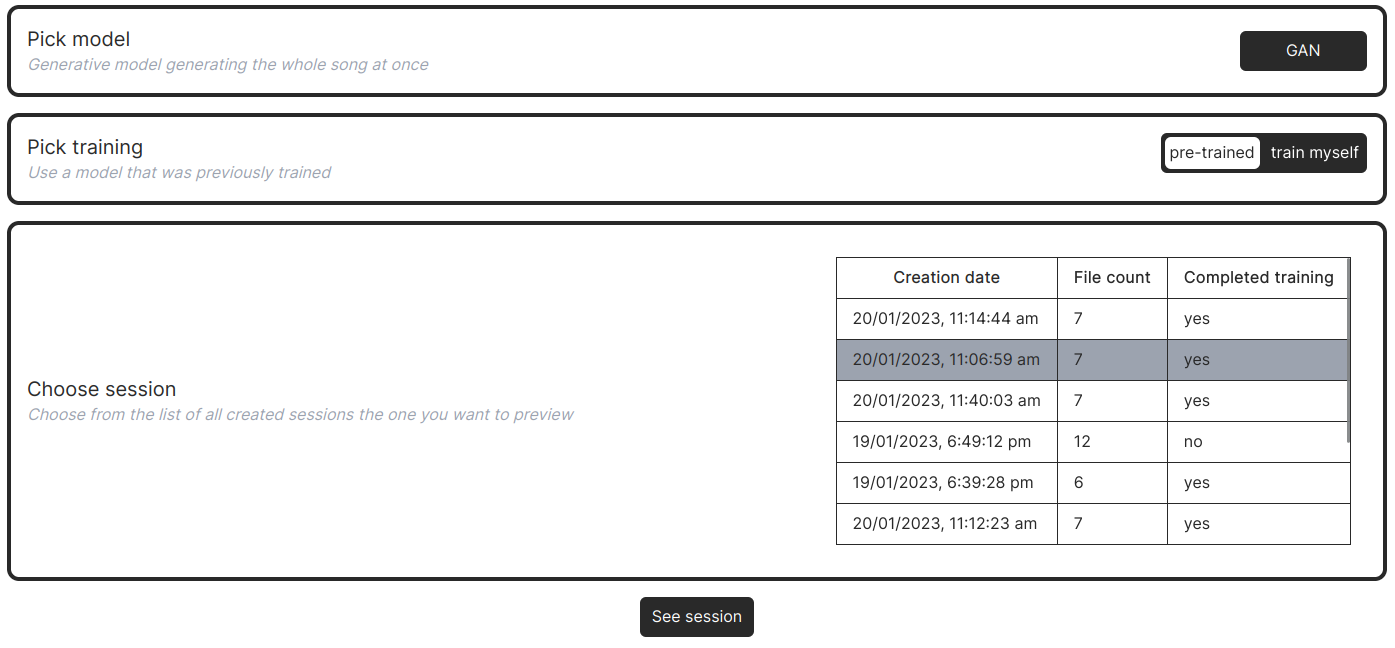
\includegraphics[width=0.98\linewidth]{gui_choose_existing_model.png}
    \caption{User interface screen allowing to pick trained model instances}
    \label{fig:gui_choose_existing_model}
\end{figure}


\section{External interfaces} \label{ex_interfaces}

External interfaces used in the project are database protocols (described in Section \ref{sec:comm_backend}) and the MIDI file format. This format is used when uploading and downloading training files. A user's dataset must be uploaded as a set of \texttt{.mid} files and cannot weigh more than 10MB. For comparison, the entire Bach training dataset (presented in Section \ref{sec:data_spec}) weighs slightly over 2MB. Additionally, we do not allow files to be nested in folders and they must not be password protected. \par
All files are asserted to be following the above conditions before running the model. Names of individual files are recorded but play no role in the execution of AI algorithms. \par


\section{Technology selection}

The main goal of the application's technology stack is to be as cross-platform as possible. That is why the selection of technologies focuses on solutions that give a possibility to abstract over the underlying platform. Nowadays, the most ubiquitous platform is arguably the Web, making it the most obvious choice for a frontend application. Thus the application is targeting the Web platform using standard cross-browser features. \par
The frontend consists of a client-side-rendered Web page distributed as a set of static JavaScript, CSS, and HTML files. Typescript\footnote{\textit{Typescript} is available at \url{https://www.typescriptlang.org/}.} language is used to build them, as it provides static types to the inherently dynamic JavaScript which is useful in safe development. To build the HTML DOM, a UI library named React\footnote{\textit{React} is available at \url{https://reactjs.org/}.} is used because it gives an unopinionated and simple approach to building user interfaces. For applying CSS, Tailwind\footnote{\textit{Tailwind} is available at \url{https://tailwindcss.com/}.} is used, but the underlying styling is custom. All variants of testing (i.e., unit, integration) are performed with the use of Vitest\footnote{\textit{Vitest} is available at \url{https://vitest.dev/}.} which is a more modern alternative to (yet compatible with) Jest\footnote{\textit{Jest} is available at \url{https://jestjs.io/}.}. Finally, to build the final output, Vite\footnote{\textit{Vite} is available at \url{https://vitejs.dev/}.} is used as it provides arguably the best developer experience and fast development cycles. Modern ECMAScript-compliant Web APIs are used to allow targeting any platform with a Web browser. \par
The backend is written as an asynchronous, multi-process Python ASGI package. This is for a simple reason: models are written in Python. Shortcomings of Python as a Web server are well understood by authors, but an executive decision to use the same language for both the models and the backend greatly simplifies their communication (it results in a direct function call, instead of an additional communication layer) was made. Given that, FastAPI\footnote{\textit{FastAPI} is available at \url{https://fastapi.tiangolo.com/}.} was chosen for creating HTTP and WebSocket APIs. FastAPI functions and \textit{pytest} package are used for software testing. To achieve better static correctness Python type hints and a type checker is used. Any platform with a Python interpreter can run this Web server, given the dependencies of the models can be resolved. Two databases are used, SQLite\footnote{\textit{SQLite} is available at \url{https://www.sqlite.org/}.} for simple persistent file-driven databases, and Redis\footnote{\textit{Redis} is available at \url{https://redis.io/}.} for streaming publish-subscribe training data. Authors believe storing full MIDI files in a database such as SQLite is a good choice, as SQLite is known for being faster than a standard file system \cite{sqlite_fs}. \par
The final component of this section is the models themselves. These are written in Python due to it being the go-to language for Machine Learning. Most Machine Learning libraries target Python and out of a crowd of candidates, Tensorflow\footnote{\textit{Tensorflow} is available at \url{https://www.tensorflow.org/}.} was chosen due to its large community support and seamless GPU/CPU interchangeability. There exist CUDA, Metal, JavaScript, WebGL, and NumPy backends for TensorFlow, so the code should work on any platform these backends can run on. \par
Finally, Docker\footnote{\textit{Docker} is available at \url{https://www.docker.com/}.} is used for deployment of the application to enable spinning up the whole project in a sandboxed environment with just a single command. The whole project also features a CI workflow ensuring that any merge commit does not break any part of the solution, and a CD workflow that deploys all changes to the production environment automatically. \par


\section{Deployment documentation}

\subsection{Hardware requirements}

Below authors present the hardware requirements for running all modules of the project. The fact that Machine Learning is a computationally expensive task is directly visible in the conditions given. Basic machines do not suffice, though it is safe to assume most personal computers (as of January 2023) can run the solution. Using an NVIDIA GPU noticeably speeds up training of selected models. \par
The requirements are:

\begin{enumerate}
    \item A 64-bit operating system,
    \item A processor (CPU): x86 or ARM architecture, and at least four threads,
    \item Memory (RAM): at least 6GB of free space,
    \item Storage (disk): at least 5GB of free space,
    \item A keyboard and a mouse to provide input,
    \item Optionally, but advisory: an NVIDIA GPU, GTX 650 or better.
\end{enumerate} \par


\subsection{Software requirements} \label{sec:software_deps}

Software requirements for launching the application include languages and libraries but do not list Docker, mentioned in Section \ref{sec:installation}. After following the installation instruction, Docker handles all languages and libraries' dependencies presented below, so there is no need to perform steps 2 to 8 manually. \par
The requirements are:

\begin{enumerate}
    \item A modern browser (e.g., \textit{Firefox}, \textit{Chrome}, \textit{Edge}, \textit{Brave}),
    \item \textit{Python}, version 3.10 (available at \url{https://www.python.org/downloads/}),
    \item \textit{pip}, version 21.0.0 or newer (available at \url{https://pypi.org/project/pip/}),
    \item \textit{pipenv}, version 2022.3.23 or newer (available at \url{https://pypi.org/project/pipenv/}),
    \item Python libraries: \textit{numpy} (1.23.5), \textit{keras} (2.10.0), \textit{tensorflow} (2.10.0), \textit{fastapi}, \textit{hypercorn}, \textit{mido}, \textit{music21}, \textit{websockets}, \textit{requests},
    \item \textit{Node.js}, version 19.0.0 or newer (available at \url{https://nodejs.org/en/}),
    \item JavaScript libraries: \textit{react} (18.2.0), \textit{typescript} (4.9.4), \textit{vite} (4.0.2), \textit{react-dom} (18.2.0), \textit{clsx} (1.2.1), \textit{react-router-dom} (6.5.0), \textit{ts-routes} (2.0), \textit{recharts} (2.2.0),
    \item \textit{Redis}, version 7.0.0 or newer (available at \url{https://redis.io/}).
\end{enumerate} \par

\subsection{Configuration}

Since the application consists of the backend and the frontend, there is a need for configuration to establish their connection. Options are kept minimal to ease the deployment. \par

\subsubsection{Port configuration}

The backend and the frontend are free to work on any available port. To configure the running port for the backend, pass the binding flag to \verb|hypercorn| when starting it manually in the \verb|./backend| folder. An example of binding to port 3030:

\verb|pipenv run hypercorn app.app --bind 0.0.0.0:3030| \par

To configure the port for frontend, when starting it manually in the \verb|./web| folder pass the port flag to \verb|vite|, example (binding to port 3030):

\verb|npm run dev -- --port 3030| \par

\subsubsection{Backend address configuration}

The frontend must know where the backend is located. Therefore, there is a single environment variable called \verb|VITE_API_URL| which points to an address of the backend. This variable is read when building the application. An important fact is, this address should not include the communication scheme. That is, instead of \verb|http://example.com/path|, it should be just \verb|example.com/path|. \par
One can also edit the \verb|./web/.env| file to set the \verb|VITE_API_URL| environment variable. \par

\subsubsection{Redis}

Connection to the Redis server goes through its own protocol, so a communication path has to be established as well. There are two environment variables controlling a connection address called \verb|REDIS_HOSTNAME| and \verb|REDIS_PORT| which respectively store a hostname and a port of the running Redis server. \par
One can also edit the \verb|./backend/.env| file to set environmental variables. \par

\subsubsection{Docker configuration}

When running the application using Docker instead of building it manually, all ports and addresses are configured from the \verb|docker-compose.yml| file. To change the backend port one must modify \verb|services.backend.ports| by setting a preferred port. Similarly, to change the frontend port one must modify \verb|services.web.ports|. An example of setting an exposed port to 1234:

\begin{verbatim}
    ports:
        - 127.0.0.1:1234:80
\end{verbatim} \par

To change the backend address one must modify \verb|services.web.build.args.VITE_API_URL|. \par


\section{Installation instruction} \label{sec:installation}

The application is fully containerized using Docker, which means the whole project can be built with a single command while having Docker installed on a computer only. \par
To install and run the application, the following steps must be followed:

\begin{enumerate}
    \item Visit \url{https://github.com/piotrowskv/music_generation} and clone the project code using \verb|git clone|,
    \item Download and install Docker (available at \url{https://www.docker.com/}),
    \item In the cloned repository, run command \verb|docker compose up|,
    \item Click on the port indicated by Docker to see the application (as presented in \figref{docker}).
\end{enumerate} \par

\begin{figure}
    \centering
    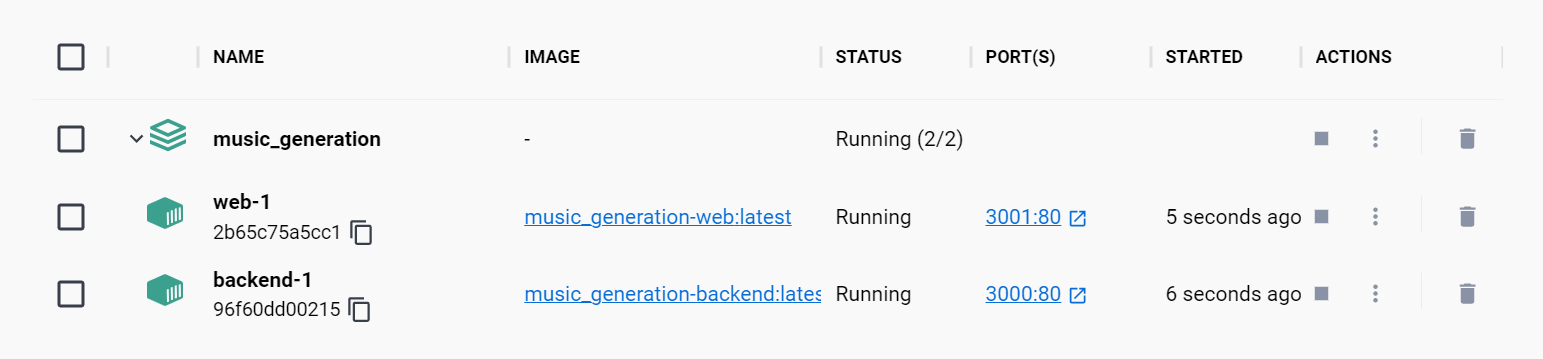
\includegraphics[width=0.8\textwidth]{assets/docker_sample.png}
    \caption{View of Docker after launching the application}
    \label{fig:docker}
\end{figure}

After performing all the actions the project is running and can be accessed in the browser by visiting the address \verb|http://localhost:3000|. \par

\subsection{Manual compilation}

Instead of using Docker, one can manually install all dependencies listed in Section \ref{sec:software_deps}. Those steps will are outlined below. While setting the backend, the following commands must be used to install libraries and build the server:

\begin{verbatim}
    pipenv install
    pipenv run python main.py
\end{verbatim} \par

However, the Redis server must be started beforehand. This is most easily done (and recommended by Redis themselves) using Docker by issuing the \verb|docker run -p 6379:6379| \verb|-it redis/redis-stack:latest| command. \par
While setting the frontend, the following commands must be used to install libraries and build the Web server:

\begin{verbatim}
    npm install
    npm run dev
\end{verbatim} \par

\subsection{Deployed version}

The application is continuously built and deployed to be accessible online at \url{https://piotrowskv.github.io/music_generation} (as of January 2023). \par



\chapter{Evaluation of application}

This chapter is devoted to correctness and means of numerical as well as subjective evaluation of the application and the models (with respect to the chosen dataset). Due to the distinctiveness of the way the models consume and produce data, their evaluation must be considered separately. A common metric is their accuracy, but it is interpreted differently for each model, therefore a direct comparison is not applicable. Standard software evaluation's scope and procedures are also mentioned briefly. \par


\section{Software testing}

The application contains test suites for various modules. The MIDI module contains tests verifying the correctness of both encoding and decoding in various configurations which were needed during development. The backend module tests its endpoints and integration between its sub-modules such as the models and the database. The frontend module has to ensure that the internal state management of the Web page works correctly as well as the connection to the backend can be established. This is verified by employing unit and integration tests. Complicated machine learning models are notoriously hard to test for correctness, hence why they are evaluated using metrics explored further in this chapter. \par


\section{Selected metrics}

Three metrics were selected to be used in the models' evaluation, as presented in the next subsections. \par

\subsection{Loss function}

A loss function is a target function of a Machine Learning model which serves as the goal to be optimized. This function has most often real numbers as the co-domain and is expressed alongside a minimization problem. Loss functions between models should not be compared, for they can be computed by extremely different methods. Complex models rarely reach a loss of zero, but a trend toward this value is a good indicator that they are learning expected properties. \par

\subsection{Accuracy}

Accuracy is a metric that evaluates the ratio between correctly predicted labels and the total number of samples (presented in Equation \ref{eq:accuracy}). Having accuracy equal to $1.0 = 100\%$ means that a model predicted all outcomes correctly. \par

\begin{equation}
    \textit{Accuracy} = \frac{\textit{Number of correct predictions}}{\textit{Total number of predictions}} \label{eq:accuracy}
\end{equation}

\subsection{\texorpdfstring{$\text{F}_1$}{F1} score}

The F$_1$ score measures the relationship between true positive (TP), true negative (TN), false positive (FP), and false negative (FN) samples. \textit{Positive} and \textit{negative} stand for predicted labels of a given sample as 1 and 0 respectively, while \textit{true} and \textit{false} indicate whether a model predicted the sample correctly. For instance, \textit{FP} means that the model \textbf{falsely} predicted the \textbf{positive} label. Other acronyms are defined analogically. \par
Firstly, we define \textit{precision} and \textit{recall} metrics in Equations \ref{eq:precision} and \ref{eq:recall}. \par

\begin{equation}
    \textit{Precision} = \frac{\textit{TP}}{\textit{TP} + \textit{FP}}
    \label{eq:precision}
\end{equation}

\begin{equation}
    \textit{Recall} = \frac{\textit{TP}}{\textit{TP} + \textit{FN}}
    \label{eq:recall}
\end{equation}

One can see that precision measures the number of correctly predicted positive samples regarding all predicted positive samples. Similarly, recall measures correctly predicted positive samples concerning the number of positive samples (in a dataset). To define the relationship between the precision and the recall, a harmonic mean of the two, called the \textit{F$_1$ score} is introduced as presented in Equation \ref{eq:f1}. \par

\begin{equation}
    \textit{F}_1 = \frac{2 \cdot \textit{Precision} \cdot \textit{Recall}}{\textit{Precision} + \textit{Recall}}
    \label{eq:f1}
\end{equation}


\subsection{ROC curve and AUC}

The receiver operating characteristic (ROC) curve describes the ratio between a false positive rate and a true positive rate. If the ratio is linear with its slope equal to 1, the classifier is considered random. A perfect classifier would have a $1.0 = 100\%$ true positive and a $0.0 = 0\%$ false positive rate. This means that curves that lean towards the left-upper corner are considered better. Visualization of exemplary ROC curves is presented in \figref{ROC_curve}. \par

\begin{figure}[H]
    \centering
    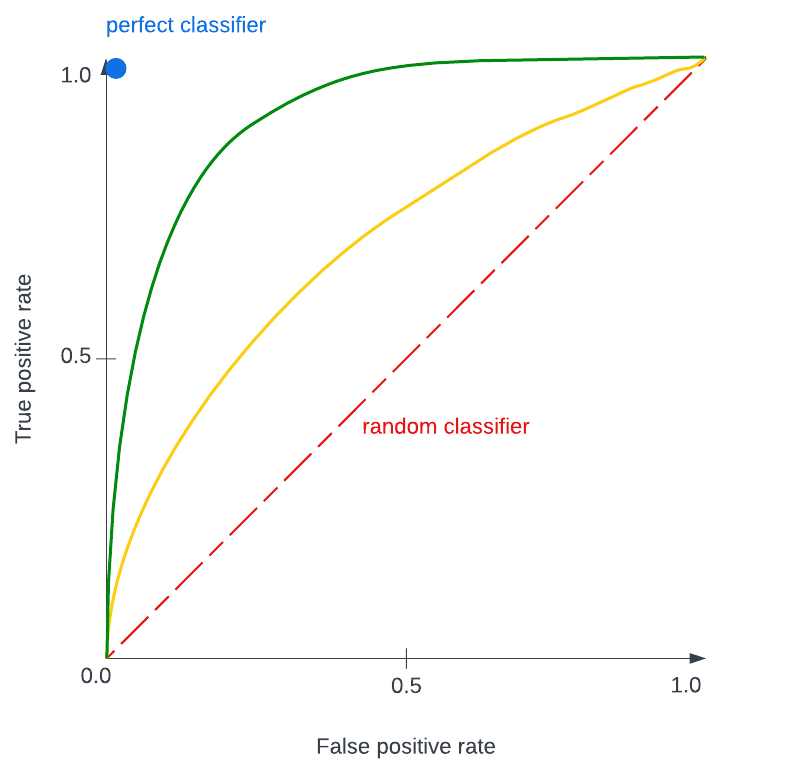
\includegraphics[width=0.5\textwidth]{assets/ROC.png}
    \caption{Examples of ROC curves}
    \label{fig:ROC_curve}
\end{figure}

The curvature is directly connected to the integral of a cumulative distribution function plotting a given ROC curve; thus, the more substantial metric is the area under the ROC curve (AUC). \par


\section{Evaluation}

In this section, the authors present an evaluation of the GAN and the LSTM models. The Markov Chain model is not included in the metrics since it does not implement any learning algorithms, so there is no possibility to improve its performance. All of the algorithms, however, are subject to unit testing, which evaluates their performance for a smaller dataset. \par

\subsection{Generative Adversarial Networks}

The GAN model is evaluated not only according to the loss function but also accuracy, the F$_1$ score, and the AUC. In addition, its discriminator is evaluated separately with shuffled data (as opposed to training on real samples first, then on fake samples). To show that it is capable of distinguishing between the two classes, the discriminator was trained separately. Fake samples for this case are taken from the previous, fully-trained generator. In GAN training, however, the discriminator is trained simultaneously with the generator. \par
A loss function of the GAN's generator and the discriminator can be seen in Figure \ref{fig:GAN-loss}. One can notice the generator having a loss function close to zero and the discriminator growing its loss function over epochs. This indicates that the generator can produce samples that are hard to distinguish for the discriminator. \par

\begin{figure}[H]
    \centering
    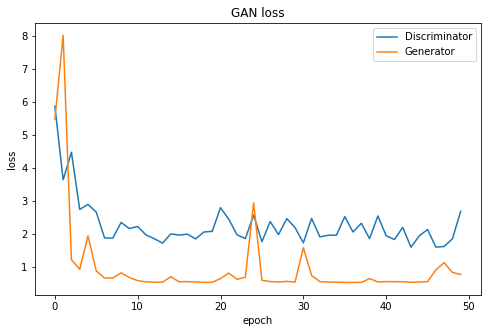
\includegraphics[width=0.7\textwidth]{assets/gan_loss.png}
    \caption{GAN model loss functions}
    \label{fig:GAN-loss}
\end{figure}

The accuracy and the F$_1$ score of the GAN model are presented in Table \ref{tab:GAN-metrics}. The AUC does not apply to this model since while evaluating generated samples, all of them belong to a single class, so the AUC equals zero. For the same reason, the generator's precision will always be either $1$ or $0$, thus the F$_1$ score will be higher than this of the discriminator. Additionally, the model does not implement a train-test split, since it evaluates its own generated samples, which are not in the dataset. \par

\begin{table}[H]
    \centering
    \caption{GAN model metrics} \vskip16pt
    \label{tab:GAN-metrics}
    \begin{tabular}{ |P{0.3\linewidth}|P{0.11\linewidth}|P{0.11\linewidth}| }
        \hline
        \small Model        & \small Accuracy & \small F$_1$ score \\
        \hline
        GAN (generator)     & 0.55            & 0.71               \\
        \hline
        GAN (discriminator) & 0.59            & 0.65               \\
        \hline
    \end{tabular}
\end{table}

Note that the perfect GAN accuracy is $0.5 = 50\%$. This means the discriminator cannot distinguish between real and fake samples. In Figures \ref{fig:GAN-acc} and \ref{fig:GAN-f1}, authors show the accuracy and F$_1$ scores for the generator and the discriminator. One can see that numbers vary during the training, but after the 25th epoch both the generator and the discriminator start to oscillate around $0.5 = 50\%$ in case of accuracy and $0.7$ in case of the F$_1$ score. \par

\begin{figure}[H]
    \centering
    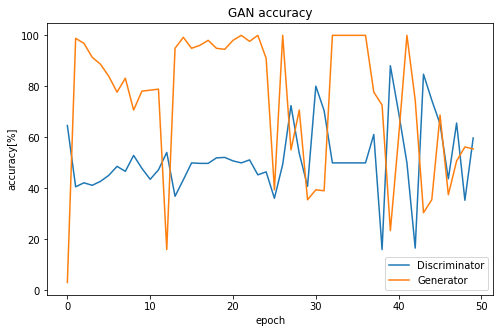
\includegraphics[width=0.7\textwidth]{assets/accuracy_gan.png}
    \caption{GAN model accuracy metrics}
    \label{fig:GAN-acc}
\end{figure}

\begin{figure}[H]
    \centering
    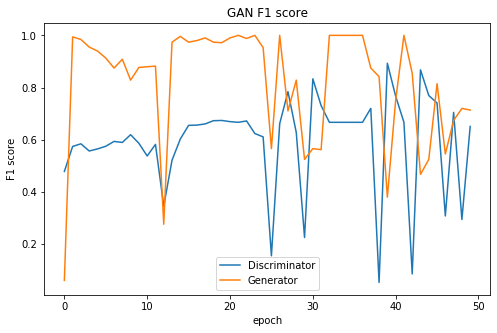
\includegraphics[width=0.7\textwidth]{assets/f1_gan.png}
    \caption{GAN model F$_1$ metrics}
    \label{fig:GAN-f1}
\end{figure}

To prove the discriminator is not completely random, Table \ref{tab:disc-metrics} shows accuracy, the F$_1$ score, and the AUC on the discriminator with the frozen, pre-trained generator. The authors conclude that the discriminator alone works well, but the GAN's architecture makes the generator adjust and learn from discriminator's results. The discriminator's accuracy along epochs is shown in Figure \ref{fig:disc-acc}. \par

\begin{table}[H]
    \centering
    \caption{Discriminator with frozen pre-trained generator metrics} \vskip16pt
    \label{tab:disc-metrics}
    \begin{tabular}{ |P{0.18\linewidth}|P{0.11\linewidth}|P{0.11\linewidth}|P{0.11\linewidth}| }
        \hline
        \small Set & \small Accuracy & \small F$_1$ score & \small AUC \\
        \hline
        Training   & 0.994           & 0.998              & 0.999      \\
        \hline
        Test       & 0.993           & 0.976              & 1.0        \\
        \hline
    \end{tabular}
\end{table}

\begin{figure}[H]
    \centering
    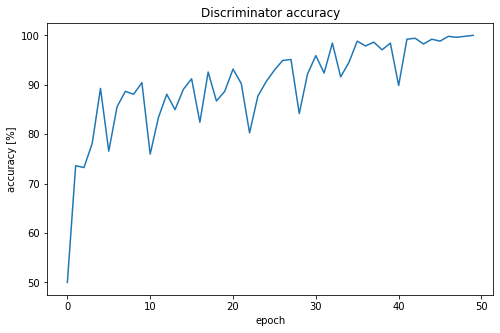
\includegraphics[width=0.7\textwidth]{assets/discriminator_acc.png}
    \caption{Discriminator-only training accuracy}
    \label{fig:disc-acc}
\end{figure}

\subsection{Long Short-Term Memory}

The first metric to be considered is the loss function. Here, it is computed using the mean squared error between predicted and expected notes. The dataset is split into three: training (72\% of the original set size), validation (8\%), and test (20\%) sets. The validation loss is also tracked during training to observe potential overfitting. Despite an initially rocky start, as seen on \figref{lstm_loss}, the loss steadily decreases for both the training and the validation set. No overfitting is observed. The test set loss is equal to $0.0155$ which is similar to that of the training one. This shows that the model generalizes well. \par

Another metric one can investigate is the accuracy of predictions. Here, a prediction is the inference of a set of notes following a given sequence. Authors compare these predictions with the dataset and mark how many of them match with the ground truth. As seen on \figref{lstm_accuracy}, the accuracy steadily increases but does not reach values typical for classification problems. After 20 epochs of training, the accuracy of $17.2\%$ and $14.2\%$ is reached for the training and the validation sets, respectively. This accuracy is considered good, as this model is meant to learn the structure of music, not to replicate given sequences perfectly. After all, unlike in typical classification problems, there is no single correct answer to a prediction here, as many notes may fit a sequence and form a harmonic melody. Finally, the accuracy for the test set is determined to be $14.7\%$. Again, no significant overfitting is observed.

\begin{figure}[H]
    \centering
    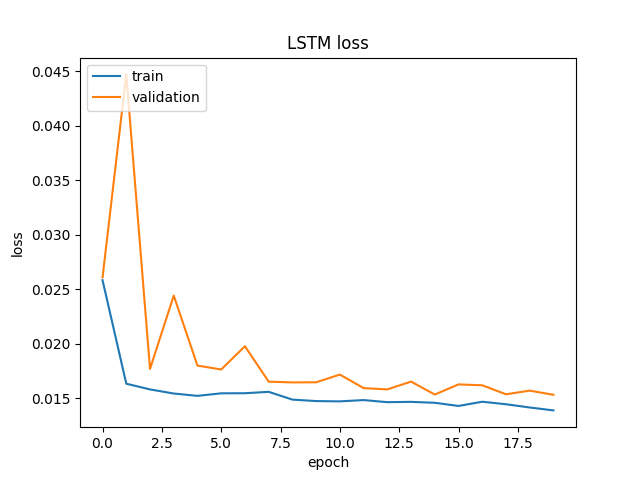
\includegraphics[width=0.7\textwidth]{lstm_loss.png}
    \caption{LSTM model loss during training}
    \label{fig:lstm_loss}
\end{figure}

\begin{figure}[H]
    \centering
    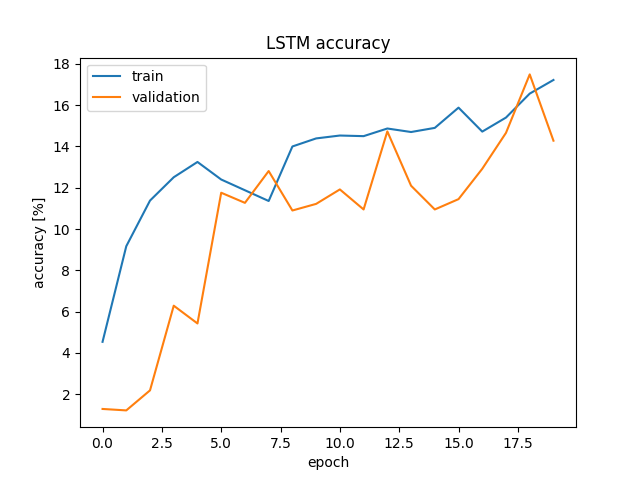
\includegraphics[width=0.7\textwidth]{lstm_accuracy.png}
    \caption{LSTM model accuracy during training}
    \label{fig:lstm_accuracy}
\end{figure}


\section{Selected compositions}

Although the numerical results of the models' evaluation can be improved, generated samples are considered by the authors to be satisfactory. This section is devoted to the presentation of the best of them. These examples are uploaded in the MIDI format to \url{https://github.com/piotrowskv/music\_generation} (as of January 2023). \par

\subsection{Generative Adversarial Networks}

Samples generated by the GAN model usually vary from one to another, depending on the size of the latent dimension. Authors observed that the GAN can produce a structurally consistent pattern, presentable as a single melodic line. However, due to the model's limitations, generated samples passed to the discriminator as \textit{real} often do not resemble music composed by professionals. Nevertheless, most of the samples can easily be played by a \textit{human} pianist. A fragment of a generated sample is shown in \figref{gan-sample}. \par

\begin{figure}[H]
    \begin{center}
        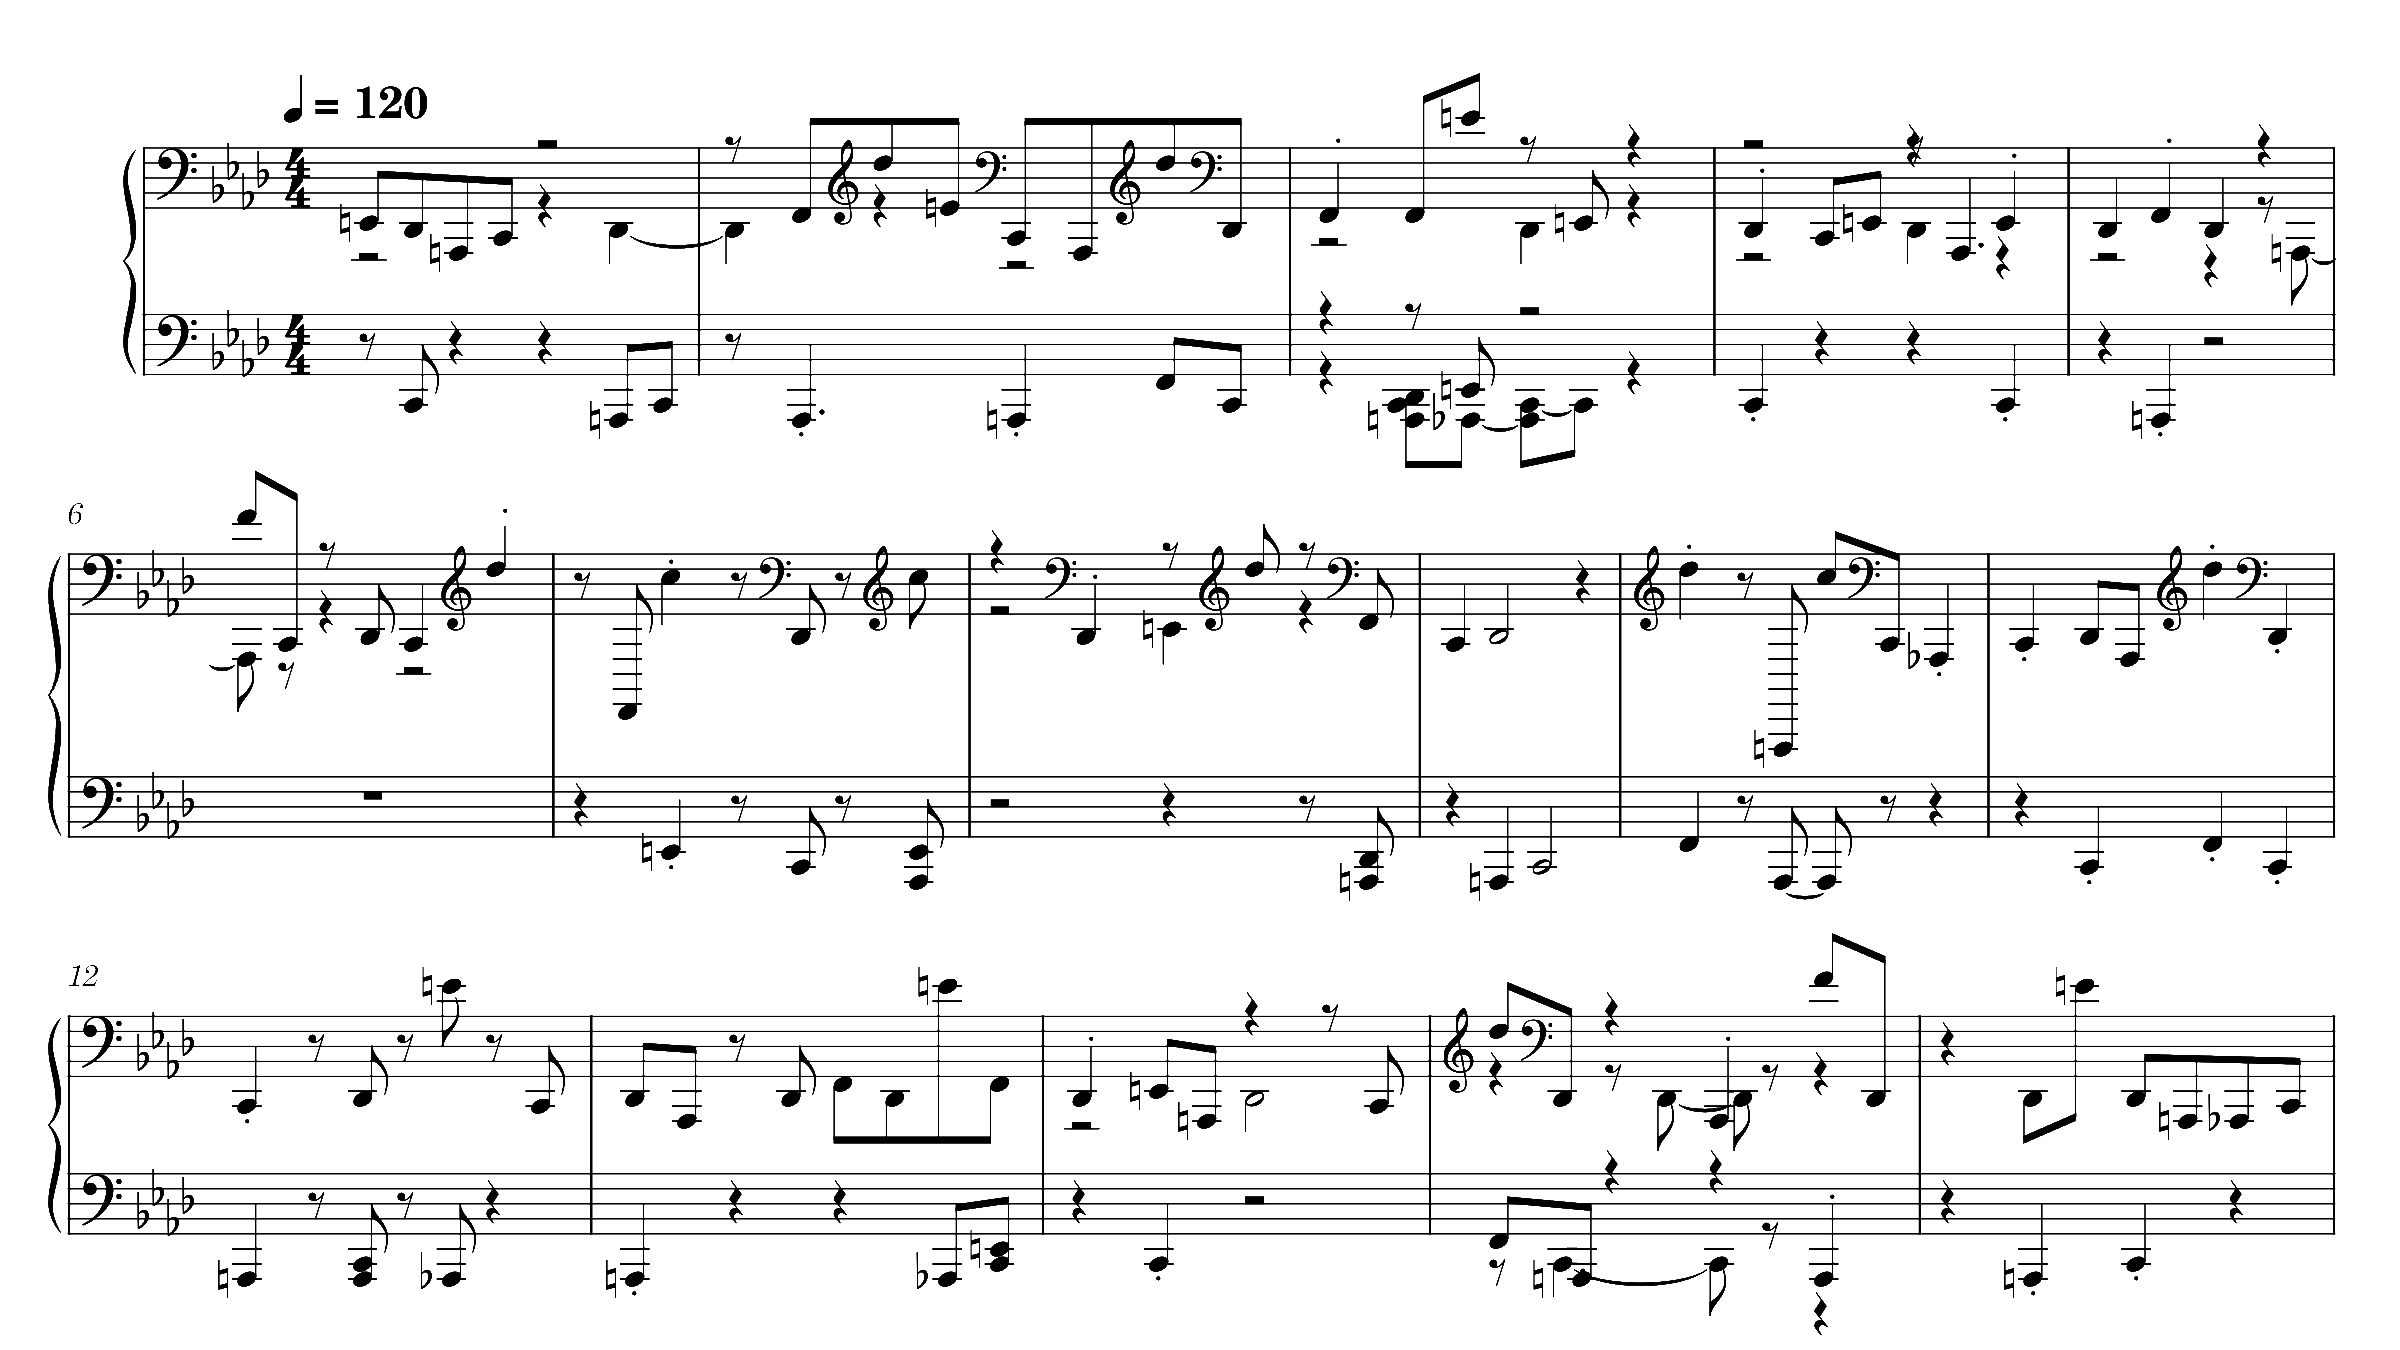
\includegraphics[width=0.9\textwidth]{gan_sample.png}
        \caption{Fragment of a sample generated by the GAN model}
        \label{fig:gan-sample}
    \end{center}
\end{figure}

\subsection{Long Short-Term Memory}

Samples generated from the LSTM model have subsequent notes close to each other. This is reflective of how real compositions are formed. A generated sample contains repetitions and occasional harmonic melodies. The lack of note duration consideration greatly affects the possibilities of this model, and this is visible in music generated. Each note being struck for the same amount of time produces very monotone sounds. Samples generated from this model are noticeably better than just sticking random notes. One such sample is shown in \figref{lstm-sample}. \par

\begin{figure}[H]
    \begin{center}
        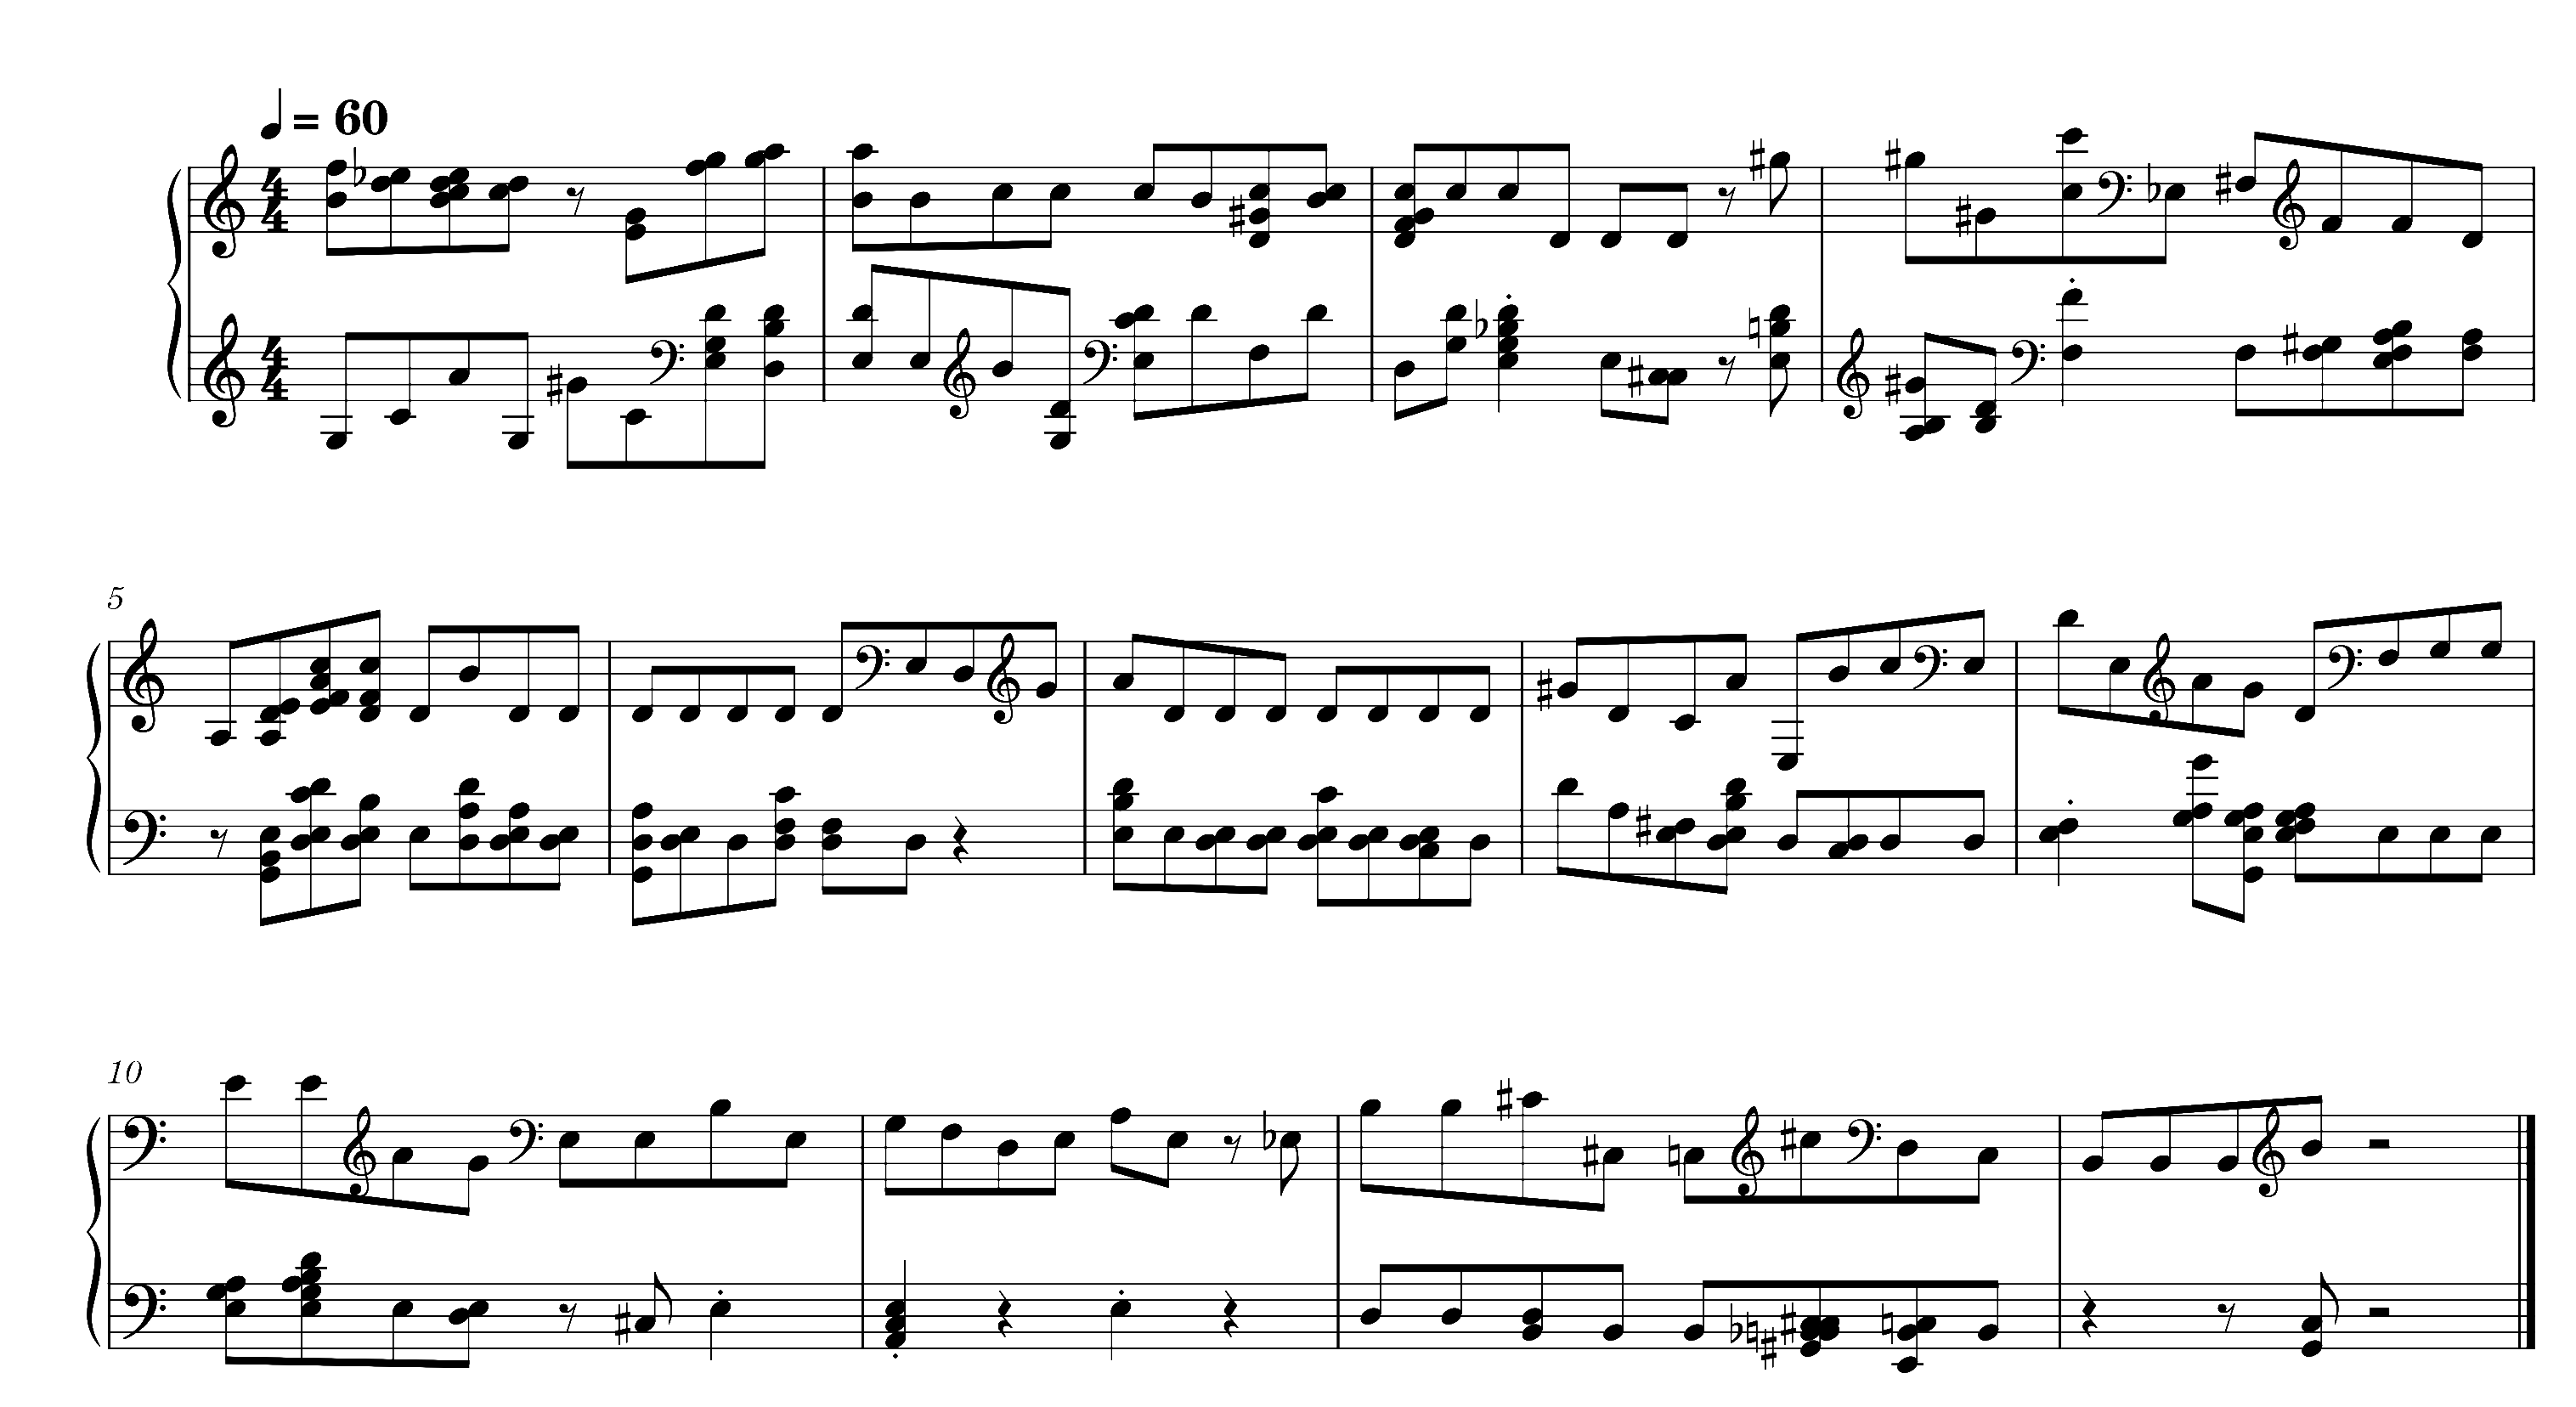
\includegraphics[width=0.9\textwidth]{lstm_sample.png}
        \caption{Sample generated by the LSTM model}
        \label{fig:lstm-sample}
    \end{center}
\end{figure}

\subsection{Markov Chains}

Samples produced using Markov Chains tend to converge to a common sequence of notes. This situation is predictable, since this model uses statistical probabilities only, so the sequence (as shown in \figref{markov_diagram}) is very probable to come full circle. A fragment of a sample generated by the Markov Chain model is shown in \figref{markov-sample}. \par


\section{Remarks and conclusions}

All models yield satisfactory results, however, there is a lot of room for improvement. Generated samples do not sound like random notes and do not resemble the original dataset. All considered models show their strengths and limitations. GANs take a long time to train, and their nature makes it hard to measure outputs numerically. LSTMs have the advantage of operating on time series and are relatively fast to train. Markov Chains are the easiest to implement, but due to their lack of inference of the structure of music, they produce crude samples. \par
Further work could consider tuning model architectures and hyperparameters, manual post-processing of samples, or defining new models. Due to the generic nature of the application new models can be easily integrated into the entire system given that they implement the common interface. Another improvement to be considered is increasing the number of features analyzed by the models, e.g., suddenly changing tempo. On the application side, authors could implement the ability to configure model parameters before training begins. \par

\begin{figure}[t]
    \begin{center}
        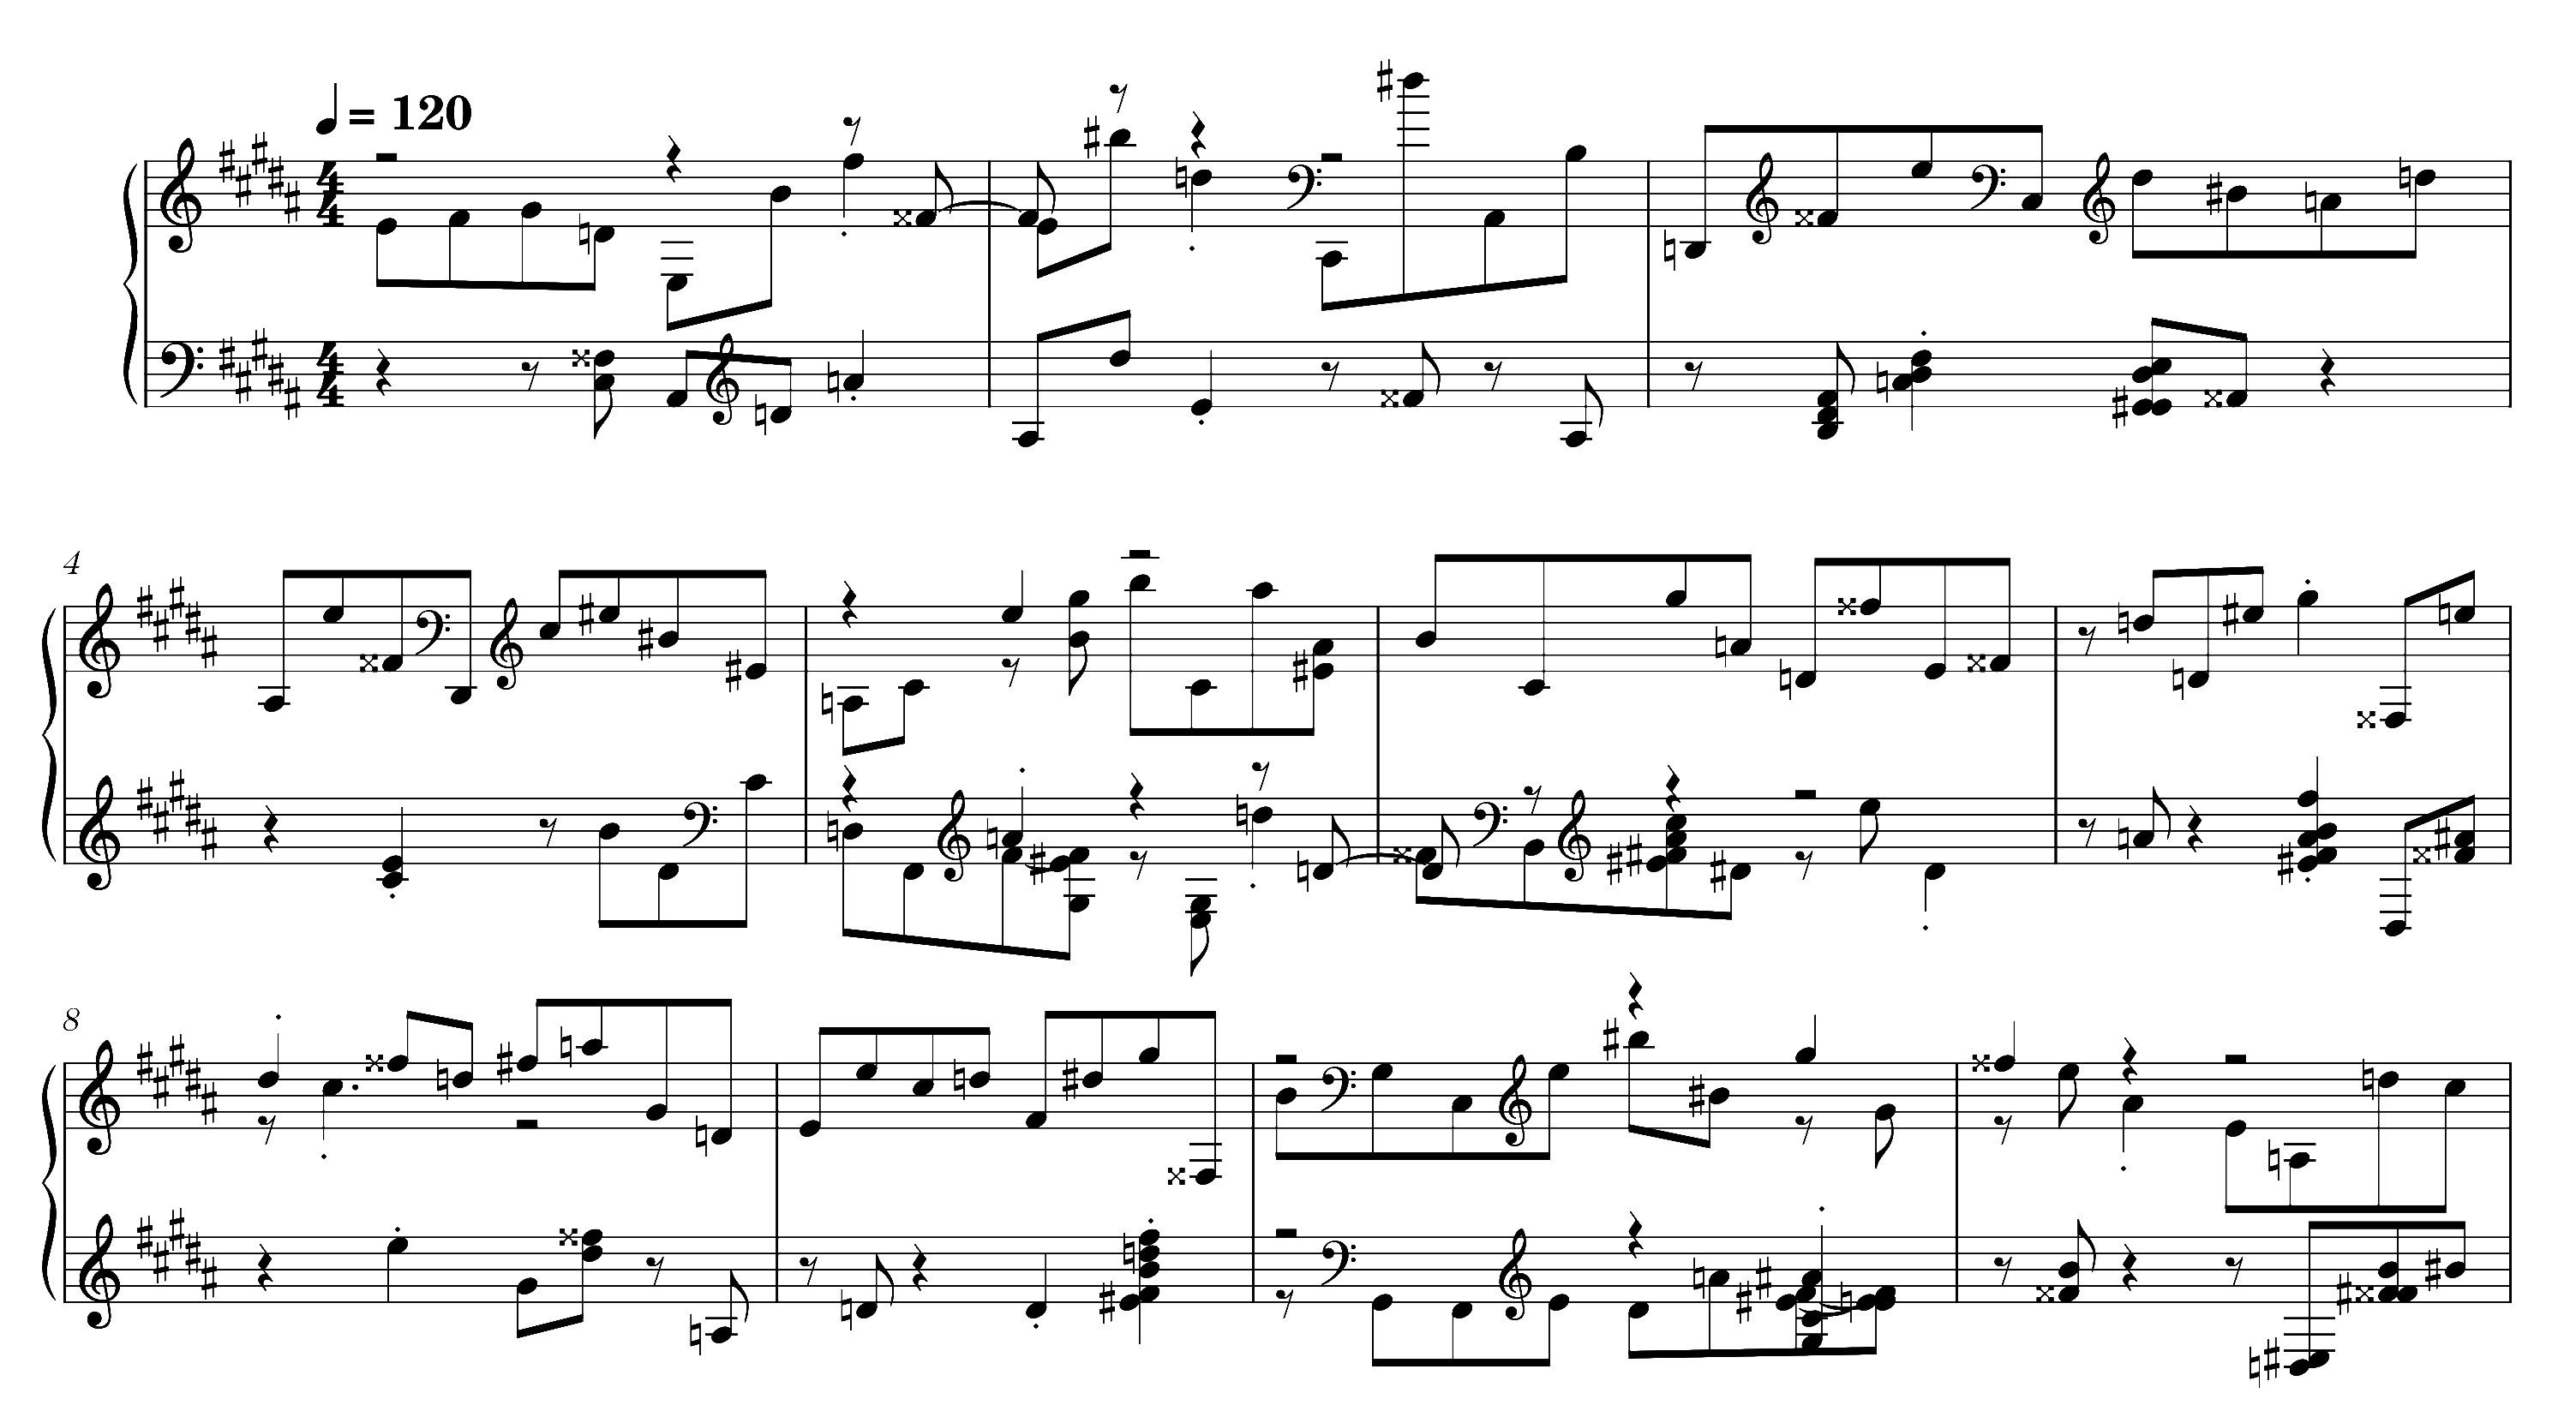
\includegraphics[width=0.9\textwidth]{markov_sample.png}
        \caption{Fragment of a sample generated by the Markov Chain model}
        \label{fig:markov-sample}
    \end{center}
\end{figure}



\chapter*{Summary}
\markboth{}{Summary}
\addcontentsline{toc}{chapter}{Summary}

The authors achieved the main goal of the thesis, which is to build an application that enables a user to generate music. This was accomplished by adapting the MIDI format characteristics as well as designing and implementing the application with its selected models. The results presented by the authors show that the models can generate music with acceptable quality. Furthermore, the Web application is fully functional and meets all defined requirements -- it allows a user to test the models on his or her dataset. \par
Both the neural networks (GAN, LSTM) and the statistical model (Markov Chain) presented in the thesis generated satisfactory samples based on the initial dataset. The models were deeply examined to select the best architecture and parameters for the given problem, with results visible through the evaluation metrics. Each of the methods has its strengths and weaknesses and the comparison between generated samples is purely subjective. What is worth noticing is all the models generated different pieces, showing that the chosen model has a crucial impact on what is going to be generated. \par
A limitation self-imposed by authors to limit the training dataset to one composer (J. S. Bach) turned out to be restrictive while developing the models in terms of possibilities of testing different data configurations (e.g., dividing the dataset concerning the number of tracks in files). The most challenging factor to the size of this set (184 files) was the availability of data online and its quality. Despite the MIDI standard having been established for around 40 years, most sheet music of well-known composers still has not made it to the public domain in this digitalized notation system. \par
Due to the restrictiveness of the development plan, the authors did not test the application against other data to challenge the foundation of the chosen set. It is likely to see an improvement in scores shown in this paper after increasing the amount of data used in models' testing. Authors plan to test presented models using datasets of different granularities (e.g., multiple composers, different genres) in the future. Further work may also include adding new models and extra tuning of the existing ones. Additionally, authors can extend the application with additional components to lift its usability, for example by adding user accounts with a personal history of trained models. \par
To conclude, there is plenty of potential in the approach to music generation presented in this thesis, and while the paper covers a fraction of the topic, there is room for development and improvements. At this stage of development, the authors do not recommend the application to be used instead of state-of-the-art alternatives, yet we encourage readers of this thesis as well as music enthusiasts to try it via the resources mentioned in the thesis. \par

\newpage

% ------------------------------- BIBLIOGRAPHY ---------------------------

% LEXICOGRAPHICAL ORDER BY AUTHORS' LAST NAMES

\markboth{Bibliography}{Bibliography}
\phantomsection
\addcontentsline{toc}{chapter}{Bibliography}

\nocite{*}
\printbibliography

\newpage

% ------------------------------- VOCABULARY ---------------------------

% PLEASE KEEP THE ALPHABETICAL ORDER!

\chapter*{Vocabulary}
\markboth{Vocabulary}{Vocabulary}
\addcontentsline{toc}{chapter}{Vocabulary}
\label{sec:vocab}

\vskip5pt \noindent
\textbf{Acceptance criteria} (abbr. \textbf{AC}) -- a set of conditions the system must fulfill to be accepted by a user story agent (e.g., user, customer, administrator). Once requirements are satisfied, the user story can be considered done and closed.

\vskip5pt \noindent
\textbf{Artificial Intelligence} (abbr. \textbf{AI}) -- the capacity of machines (inter alia computers) to exhibit or simulate intelligent behavior; also a field of study concerning these capacities \cite{AI_OED}.

\vskip5pt \noindent
\textbf{(Artificial) neural network} (abbr. \textbf{ANN} or \textbf{NN}) -- in Computer Science, an algorithmic structure which is the core of deep learning algorithms. Its name and structure are inspired by the human brain, mimicking how biological neurons communicate with one another \cite{NN_IBM}.

\vskip5pt \noindent
\textbf{Asynchronous Server Gateway Interface} (abbr. \textbf{ASGI}) -- a calling convention for request forwarding for asynchronous Python servers.

\vskip5pt \noindent
\textbf{Bach-Werke-Verzeichnis} (abbr. \textbf{BWV}, lit. \textit{Bach Works Catalogue}) -- a listing of Johann Sebastian Bach's compositions created in 1950 by Wolfgang Schmieder, with subsequent editions from 1990 and 1998. Works in the catalog are sorted by genre and target instruments.

\vskip5pt \noindent
\textbf{Convolutional Neural Network} (abbr. \textbf{CNN}) -- a neural network architecture implementing convolutional layers, mostly used in image processing \cite{CNN}.

\vskip5pt \noindent
\textbf{Fortepiano} -- an early version and a direct predecessor of the piano, created in 1698 by Bartolomeo Cristofori. It has a lower tonal range (at least four octaves) that the current-era piano (seven-and-a-third octaves).

\vskip5pt \noindent
\textbf{Harpsichord} -- a 14th-century piano-like instrument with its strings being plucked instead of being struck after hitting the keyboard.

\vskip5pt \noindent
\textbf{Machine Learning} (abbr. \textbf{ML}) -- a branch of Artificial Intelligence which focuses on the use of data and algorithms to imitate the way that humans learn by gradual improvements of success rate \cite{ML_IBM}.

\newpage

% ----------------------- LIST OF ABBREVIATIONS ------------------

\chapter*{List of abbreviations and acronyms}
\markboth{List of abbreviations and acronyms}{List of abbreviations and acronyms}
\addcontentsline{toc}{chapter}{List of abbreviations and acronyms}

\begin{longtable}{cl}
    AC      & Acceptance criteria \textit{(see Vocabulary)}                   \\
    AI      & Artificial Intelligence \textit{(see Vocabulary)}               \\
    API     & Application Programming Interface                               \\
    ARM     & Advanced RISC Machine                                           \\
    ASGI    & Asynchronous Server Gateway Interface \textit{(see Vocabulary)} \\
    AUC     & Area under (the ROC) curve                                      \\
    BWV     & Bach-Werke-Verzeichnis \textit{(see Vocabulary)}                \\
    CD      & Continuous deployment                                           \\
    CI      & Continuous integration                                          \\
    Conv    & Convolution                                                     \\
    CPU     & Central processing unit                                         \\
    CQRS    & Command Query Responsibility Segregation                        \\
    CSS     & Cascading Style Sheets                                          \\
    CUDA    & Compute Unified Device Architecture                             \\
    DOM     & Document Object Model                                           \\
    FN      & False negative                                                  \\
    FP      & False positive                                                  \\
    GAN     & Generative Adversarial Network                                  \\
    GB      & Gigabyte \textit{(1GB = 1,000MB)}                               \\
    GPU     & Graphics processing unit                                        \\
    GTX     & Giga Texel Shader eXtreme                                       \\
    GUI     & Graphical user interface                                        \\
    HEX     & Hexadecimal                                                     \\
    HTTP(S) & Hypertext Transfer Protocol (Secure)                            \\
    KB      & Kilobyte \textit{(1KB = 1,000 bytes)}                           \\
    LSTM    & Long Short-Term Memory                                          \\
    MB      & Megabyte \textit{(1MB = 1,000KB)}                               \\
    MIDI    & Musical Instrument Digital Interface                            \\
    MP3     & MPEG-1/MPEG-2 Audio Layer III                                   \\
    PC      & Personal computer                                               \\
    PDF     & Portable Document Format                                        \\
    RAM     & Random access memory                                            \\
    ReLU    & Rectified linear unit (activation function)                     \\
    REST    & Representational state transfer                                 \\
    RNN     & Recurrent Neural Network                                        \\
    ROC     & Receiver operating characteristic                               \\
    SWOT    & Strengths, weaknesses, opportunities, threats                   \\
    TN      & True negative                                                   \\
    TP      & True positive                                                   \\
    UI      & User interface                                                  \\
    URPS    & Usability, reliability, performance, supportability             \\
    WS(S)   & WebSocket (Secure)                                              \\
\end{longtable}

\newpage

% ----------------------------  LIST OF FIGURES --------------------------------

\phantomsection
\addcontentsline{toc}{chapter}{List of figures}
\listoffigures

\newpage

% -----------------------------  LIST OF TABLES --------------------------------

\renewcommand{\listtablename}{List of tables}
\phantomsection
\addcontentsline{toc}{chapter}{List of tables}
\listoftables

\newpage

% -----------------------------  LIST OF APPENDICES ---------------------------

\chapter*{List of appendices}
\markboth{List of appendices}{List of appendices}
\addcontentsline{toc}{chapter}{List of appendices}

\begin{enumerate}
    \item Appendix \ref{app:work}: Work division
    \item Appendix \ref{app:notes}: MIDI notes
    \item Appendix \ref{app:dataset}: Dataset content
\end{enumerate}

\newpage

% -----------------------------  APPENDICES --------------------------------

\appendix
\setcounter{table}{0}
\renewcommand{\thetable}{A.\arabic{table}}

\chapter{Work division} \label{app:work}

Table \ref{tab:work-division} presents the distribution of tasks among the authors. The division is designed to provide equal work allocation as well as continuity of performance. Some work was done by all together -- these assignments were presented under \textit{Collective tasks}. \par

\vfill

\begin{table}[H]
    \centering
    \caption{Work division between authors} \vskip16pt
    \label{tab:work-division}
    \begin{tabular}{ |P{0.27\linewidth}|R{0.68\linewidth}| }
        \hline
        \small \setlength{\baselineskip}{5pt}Author             & \small Tasks                                                    \\
        \hline

        \setlength{\baselineskip}{5pt}\textit{Collective tasks} &
        \setlength{\baselineskip}{5pt}\begin{itemize}
                                          \setlength{\baselineskip}{5pt}    \item Project preparation
                                                \setlength{\baselineskip}{5pt}    \item Research of available datasets
                                                \setlength{\baselineskip}{5pt}    \item Unit testing
                                                \setlength{\baselineskip}{5pt}    \item Integration testing
                                                \setlength{\baselineskip}{5pt}    \item System testing
                                                \setlength{\baselineskip}{5pt}    \item Final corrections and system review
                                                \setlength{\baselineskip}{5pt}\end{itemize}                  \\
        \hline

        \setlength{\baselineskip}{5pt}Szymon Górski             &
        \setlength{\baselineskip}{5pt}\begin{itemize}
                                          \setlength{\baselineskip}{5pt}    \item Choice of datasets to be included and accessing them
                                                \setlength{\baselineskip}{5pt}    \item Implementation of MIDI transcription module
                                                \setlength{\baselineskip}{5pt}    \item LSTM model development
                                                \setlength{\baselineskip}{5pt}\end{itemize} \\
        \hline

        \setlength{\baselineskip}{5pt}Weronika Piotrowska       &
        \setlength{\baselineskip}{5pt}\begin{itemize}
                                          \setlength{\baselineskip}{5pt}    \item GAN model development
                                                \setlength{\baselineskip}{5pt}    \item Markov Chain model development
                                                \setlength{\baselineskip}{5pt}    \item Efficiency and quality comparison of AI models
                                                \setlength{\baselineskip}{5pt}\end{itemize}       \\
        \hline

        \setlength{\baselineskip}{5pt}Marcin Wojnarowski        &
        \setlength{\baselineskip}{5pt}\begin{itemize}
                                          \setlength{\baselineskip}{5pt}    \item Client-server application development
                                                \setlength{\baselineskip}{5pt}    \item Graphical user interface design and implementation
                                                \setlength{\baselineskip}{5pt}    \item Application integration with AI models
                                                \setlength{\baselineskip}{5pt}    \item LSTM model development
                                                \setlength{\baselineskip}{5pt}\end{itemize}   \\
        \hline
    \end{tabular}
\end{table} \par

\vfill
\newpage

\chapter{MIDI notes} \label{app:notes}
\setcounter{table}{0}
\renewcommand{\thetable}{B.\arabic{table}}

Sheet music notes are translated to MIDI notes by assigning integers to subsequent values, beginning with 0 for the C-1 note and ending with 127 for the G\#9 note. No notes outside this range are supported. MIDI files, unless overruled by a message, implicitly define A4 note frequency as 440 Hz, compliant with ISO 16 standard (sometimes referred to as A440) \cite{MIDI1_spec}. Historically, the frequency of the A4 note has not been constant and it is believed that Bach's music should be performed with the \textit{baroque pitch} of 415 Hz \cite{Bach_dict}. The formula for other notes' frequencies is:

\begin{equation}
    f = f_{\text{A4}} \cdot 2^{\left (\frac{n - 69}{12} \right )}
\end{equation} \par

Table \ref{tab:octave} presents correspondence of music notation with MIDI notes assigned, respectively.  \par

% a phantom table to put caption before a table (\longtable doesn't support well \caption at the beginning of its body) - page numbering issue

\begin{table}[H]
    \caption{Translation of notes from the fourth octave to MIDI notes \cite{MIDI_notes}}
    \label{tab:octave}
\end{table}
\addtocounter{table}{-1}

\begin{longtable}{ | M{3.5cm} | M{2.8cm} | M{2.8cm} | M{2.5cm} | M{2.2cm} | }
    \hline
    \small Representation(s)                                     & \small English notation & \small German notation & \small Frequency   & \small MIDI Note \\
    \hline
    \endhead
    
\includegraphics[width=0.85\linewidth]{assets/notes/C4.png}  & C4                      & c'                     & 261.63 Hz          & 60               \\ \hline
    
\includegraphics[width=0.85\linewidth]{assets/notes/CS4.png} & C\#4/Db4                & cis'/des'              & 277.18 Hz          & 61               \\ \hline
    
\includegraphics[width=0.85\linewidth]{assets/notes/D4.png}  & D4                      & d'                     & 293.66 Hz          & 62               \\ \hline
    
\includegraphics[width=0.85\linewidth]{assets/notes/DS4.png} & D\#4/Eb4                & dis'/es'               & 311.13 Hz          & 63               \\ \hline
    
\includegraphics[width=0.85\linewidth]{assets/notes/E4.png}  & E4                      & e'                     & 329.63 Hz          & 64               \\ \hline
    
\includegraphics[width=0.85\linewidth]{assets/notes/F4.png}  & F4                      & f'                     & 349.23 Hz          & 65               \\ \hline
    
\includegraphics[width=0.85\linewidth]{assets/notes/FS4.png} & F\#4/Gb4                & fis'/ges'              & 369.99 Hz          & 66               \\ \hline
    
\includegraphics[width=0.85\linewidth]{assets/notes/G4.png}  & G4                      & g'                     & 392.00 Hz          & 67               \\ \hline
    
\includegraphics[width=0.85\linewidth]{assets/notes/GS4.png} & G\#4/Ab4                & gis'/as'               & 415.30 Hz          & 68               \\ \hline
    
\includegraphics[width=0.85\linewidth]{assets/notes/A4.png}  & A4                      & a'                     & \textbf{440.00 Hz} & 69               \\ \hline
    
\includegraphics[width=0.85\linewidth]{assets/notes/AS4.png} & A\#4/Bb4                & ais'/b'                & 466.16 Hz          & 70               \\ \hline
    
\includegraphics[width=0.85\linewidth]{assets/notes/B4.png}  & B4                      & h'                     & 493.88 Hz          & 71               \\ \hline \hline
    
\includegraphics[width=0.85\linewidth]{assets/notes/C5.png}  & C5                      & c''                    & 523.25 Hz          & 72               \\ \hline
\end{longtable}

\newpage

\chapter{Dataset content} \label{app:dataset}
\setcounter{table}{0}
\renewcommand{\thetable}{C.\arabic{table}}

Table \ref{tab:Bach_works} contains the full register of Johann Sebastian Bach's works included in the dataset used by authors during thesis application development. Columns \textit{Dataset} and \textit{Author} present sources of files and authors of MIDI files containing respective compositions with numbers assigned as listed below. \par

\vfill

Sources of MIDI files in the dataset are:

\begin{enumerate}
    \item \textit{A Johann Sebastian Bach Midi Page} by B. Travis \cite{MIDI_central},
    \item \textit{Dave's J.S. Bach Page} by D. J. Grossman \cite{MIDI_Dave},
    \item \textit{Large collection of Classical MIDI of Bach's music} by kunstderfuge.com \cite{MIDI_kunst}.
\end{enumerate} \par

\vfill

The authors of MIDI files in the dataset are:

\begin{enumerate}
    \item G. Bricault
    \item L. Collinelli
    \item H. Fesefeldt
    \item T. L. Hubeart Jr.
    \item D. J. Grossman
    \item D. Jao
    \item J. H. McCloskey
    \item B. Travis
\end{enumerate} \par

\vfill
% a phantom table to put caption before a table (\longtable doesn't support well \caption at the beginning of its body) - page numbering issue

\newpage
\begin{table}[H]
    \caption{List of J. S. Bach work titles, corresponding MIDI files and their authors \cite{MIDI_Dave}\cite{MIDI_kunst}\cite{MIDI_central}}
    \label{tab:Bach_works}
\end{table}
\addtocounter{table}{-1}

\footnotesize
\begin{longtable}{ |S{0.37\textwidth}|P{0.12\textwidth}|P{0.09\textwidth}|P{0.09\textwidth}|S{0.21\textwidth}| }
\hline
Name & BWV & Dataset & Author & Filename(s) \\ \hline
\endhead
\multicolumn{5}{|l|}{\textbf{\textit{Two-voice Inventions}}, BWV 772-786} 														\\ \hline
\textit{Invention in C major} 										& BWV 772	& [1] 	& [8] 	& \texttt{bwv772.mid} 			\\ \hline
\textit{Invention in C minor} 										& BWV 773	& [1] 	& [8] 	& \texttt{bwv773.mid} 			\\ \hline
\textit{Invention in D major} 										& BWV 774	& [1] 	& [8] 	& \texttt{bwv774.mid} 			\\ \hline
\textit{Invention in D minor} 										& BWV 775	& [1] 	& [8] 	& \texttt{bwv775.mid} 			\\ \hline
\textit{Invention in E flat major} 									& BWV 776	& [1] 	& [8] 	& \texttt{bwv776.mid} 			\\ \hline
\textit{Invention in E major} 										& BWV 777	& [1] 	& [8] 	& \texttt{bwv777.mid} 			\\ \hline
\textit{Invention in E minor} 										& BWV 778	& [1] 	& [8] 	& \texttt{bwv778.mid} 			\\ \hline
\textit{Invention in F major} 										& BWV 779	& [1] 	& [8] 	& \texttt{bwv779.mid} 			\\ \hline
\textit{Invention in F minor} 										& BWV 780	& [1] 	& [8] 	& \texttt{bwv780.mid} 			\\ \hline
\textit{Invention in G major} 										& BWV 781	& [1] 	& [8] 	& \texttt{bwv781.mid} 			\\ \hline
\textit{Invention in G minor} 										& BWV 782	& [1] 	& [8] 	& \texttt{bwv782.mid} 			\\ \hline
\textit{Invention in A major} 										& BWV 783	& [1] 	& [8] 	& \texttt{bwv783.mid} 			\\ \hline
\textit{Invention in A minor} 										& BWV 784	& [1] 	& [8] 	& \texttt{bwv784.mid} 			\\ \hline
\textit{Invention in B flat major} 									& BWV 785	& [1] 	& [8] 	& \texttt{bwv785.mid} 			\\ \hline
\textit{Invention in B minor} 										& BWV 786	& [1] 	& [8] 	& \texttt{bwv786.mid} 			\\ \hline
\multicolumn{5}{|l|}{\textbf{\textit{Three-voice Sinfonias}}, BWV 787-801} 														\\ \hline
\textit{Sinfonia in C major} 										& BWV 787	& [1] 	& [8] 	& \texttt{bwv787.mid} 			\\ \hline
\textit{Sinfonia in C minor} 										& BWV 788	& [1] 	& [8] 	& \texttt{bwv788.mid} 			\\ \hline
\textit{Sinfonia in D major} 										& BWV 789	& [1] 	& [8] 	& \texttt{bwv789.mid} 			\\ \hline
\textit{Sinfonia in D minor} 										& BWV 790	& [1] 	& [8] 	& \texttt{bwv790.mid} 			\\ \hline
\textit{Sinfonia in E flat major} 									& BWV 791	& [1] 	& [8] 	& \texttt{bwv791.mid} 			\\ \hline
\textit{Sinfonia in E major} 										& BWV 792	& [1] 	& [8] 	& \texttt{bwv792.mid} 			\\ \hline
\textit{Sinfonia in E minor} 										& BWV 793	& [1] 	& [8] 	& \texttt{bwv793.mid} 			\\ \hline
\textit{Sinfonia in F major} 										& BWV 794	& [1] 	& [8] 	& \texttt{bwv794.mid} 			\\ \hline
\textit{Sinfonia in F minor} 										& BWV 795	& [1] 	& [8] 	& \texttt{bwv795.mid} 			\\ \hline
\textit{Sinfonia in G major} 										& BWV 796	& [1] 	& [8] 	& \texttt{bwv796.mid} 			\\ \hline
\textit{Sinfonia in G minor} 										& BWV 797	& [1] 	& [8] 	& \texttt{bwv797.mid} 			\\ \hline
\textit{Sinfonia in A major} 										& BWV 798	& [1] 	& [8] 	& \texttt{bwv798.mid} 			\\ \hline
\textit{Sinfonia in A minor} 										& BWV 799	& [1] 	& [8] 	& \texttt{bwv799.mid} 			\\ \hline
\textit{Sinfonia in B flat major} 									& BWV 800	& [1] 	& [8] 	& \texttt{bwv800.mid} 			\\ \hline
\textit{Sinfonia in B minor} 										& BWV 801	& [1] 	& [8] 	& \texttt{bwv801.mid} 			\\ \hline
\multicolumn{5}{|l|}{\textbf{\textit{Four Duets}}, BWV 802-805} 																\\ \hline
\textit{Duet in E minor} 											& BWV 802	& [2] 	& [6] 	& \texttt{bwv802.mid} 			\\ \hline
\textit{Duet in F major} 											& BWV 803	& [2] 	& [6] 	& \texttt{bwv803.mid} 			\\ \hline
\textit{Duet in G major} 											& BWV 804	& [2] 	& [6] 	& \texttt{bwv804.mid} 			\\ \hline
\textit{Duet in A minor} 											& BWV 805	& [2] 	& [6] 	& \texttt{bwv805.mid} 			\\ \hline
\multicolumn{5}{|l|}{\textbf{\textit{English Suites}}, BWV 806-811} 															\\ \hline
\textit{Suite in A major} 											& BWV 806	& [2] 	& [1] 	& \setlength{\baselineskip}{12pt}\texttt{bwv806a.mid}, \texttt{bwv806b.mid}, \texttt{bwv806c.mid}, \texttt{bwv806d.mid}, \texttt{bwv806e.mid}, \texttt{bwv806f.mid}, \texttt{bwv806g.mid}, \texttt{bwv806h.mid}, \texttt{bwv806i.mid}, \texttt{bwv806j.mid} \\ \hline
\textit{Suite in A minor} 											& BWV 807	& [2] 	& [1] 	& \setlength{\baselineskip}{12pt}\texttt{bwv807a.mid}, \texttt{bwv807b.mid}, \texttt{bwv807c.mid}, \texttt{bwv807d.mid}, \texttt{bwv807e.mid}, \texttt{bwv807f.mid}, \texttt{bwv807g.mid}, \texttt{bwv807h.mid} \\ \hline
\textit{Suite in G minor} 											& BWV 808	& [2] 	& [1] 	& \setlength{\baselineskip}{12pt}\texttt{bwv808a.mid}, \texttt{bwv808b.mid}, \texttt{bwv808c.mid}, \texttt{bwv808d.mid}, \texttt{bwv808e.mid}, \texttt{bwv808f.mid}, \texttt{bwv808g.mid}, \texttt{bwv808h.mid} \\ \hline
\textit{Suite in F major} 											& BWV 809	& [2] 	& [1] 	& \setlength{\baselineskip}{12pt}\texttt{bwv809a.mid}, \texttt{bwv809b.mid}, \texttt{bwv809c.mid}, \texttt{bwv809d.mid}, \texttt{bwv809e.mid}, \texttt{bwv809f.mid}, \texttt{bwv809g.mid} \\ \hline
\textit{Suite in E minor} 											& BWV 810	& [2] 	& [1] 	& \setlength{\baselineskip}{12pt}\texttt{bwv810a.mid}, \texttt{bwv810b.mid}, \texttt{bwv810c.mid}, \texttt{bwv810d.mid}, \texttt{bwv810e.mid}, \texttt{bwv810f.mid}, \texttt{bwv810g.mid} \\ \hline
\textit{Suite in D minor} 											& BWV 811	& [2] 	& [1] 	& \setlength{\baselineskip}{12pt}\texttt{bwv811a.mid}, \texttt{bwv811b.mid}, \texttt{bwv811c.mid}, \texttt{bwv811d.mid}, \texttt{bwv811e.mid}, \texttt{bwv811f.mid}, \texttt{bwv811g.mid}, \texttt{bwv811h.mid} \\ \hline
\multicolumn{5}{|l|}{\textbf{\textit{The Well-tempered Clavier} (Book I)}, BWV 846-869} 										\\ \hline
\textit{Prelude and Fugue in C major} 								& BWV 846	& [3] 	& [3] 	& \texttt{bwv846.mid} 			\\ \hline
\textit{Prelude and Fugue in C minor} 								& BWV 847	& [3] 	& [3] 	& \texttt{bwv847.mid} 			\\ \hline
\textit{Prelude and Fugue in C sharp major} 						& BWV 848	& [3] 	& [3] 	& \texttt{bwv848.mid} 			\\ \hline
\textit{Prelude and Fugue in C sharp minor} 						& BWV 849	& [3] 	& [3] 	& \texttt{bwv849.mid} 			\\ \hline
\textit{Prelude and Fugue in D major} 								& BWV 850	& [3] 	& [3] 	& \texttt{bwv850.mid} 			\\ \hline
\textit{Prelude and Fugue in D minor} 								& BWV 851	& [3] 	& [3] 	& \texttt{bwv851.mid} 			\\ \hline
\textit{Prelude and Fugue in E flat major} 							& BWV 852	& [3] 	& [3] 	& \texttt{bwv852.mid} 			\\ \hline
\textit{Prelude and Fugue in E flat minor} 							& BWV 853	& [3] 	& [3] 	& \texttt{bwv853.mid} 			\\ \hline
\textit{Prelude and Fugue in E major} 								& BWV 854	& [3] 	& [3] 	& \texttt{bwv854.mid} 			\\ \hline
\textit{Prelude and Fugue in E minor} 								& BWV 855	& [3] 	& [3] 	& \texttt{bwv855.mid} 			\\ \hline
\textit{Prelude and Fugue in F major} 								& BWV 856	& [3] 	& [3] 	& \texttt{bwv856.mid} 			\\ \hline
\textit{Prelude and Fugue in F minor} 								& BWV 857	& [3] 	& [3] 	& \texttt{bwv857.mid} 			\\ \hline
\textit{Prelude and Fugue in F sharp major} 						& BWV 858	& [3] 	& [3] 	& \texttt{bwv858.mid} 			\\ \hline
\textit{Prelude and Fugue in F sharp minor} 						& BWV 859	& [3] 	& [3] 	& \texttt{bwv859.mid} 			\\ \hline
\textit{Prelude and Fugue in G major} 								& BWV 860	& [3] 	& [3] 	& \texttt{bwv860.mid} 			\\ \hline
\textit{Prelude and Fugue in G minor} 								& BWV 861	& [3] 	& [3] 	& \texttt{bwv861.mid} 			\\ \hline
\textit{Prelude and Fugue in A flat major} 							& BWV 862	& [3] 	& [3] 	& \texttt{bwv862.mid} 			\\ \hline
\textit{Prelude and Fugue in G sharp minor} 						& BWV 863	& [3] 	& [3] 	& \texttt{bwv863.mid} 			\\ \hline
\textit{Prelude and Fugue in A major} 								& BWV 864	& [3] 	& [3] 	& \texttt{bwv864.mid} 			\\ \hline
\textit{Prelude and Fugue in A minor} 								& BWV 865	& [3] 	& [3] 	& \texttt{bwv865.mid} 			\\ \hline
\textit{Prelude and Fugue in B flat major} 							& BWV 866	& [3] 	& [3] 	& \texttt{bwv866.mid} 			\\ \hline
\textit{Prelude and Fugue in B flat minor} 							& BWV 867	& [3] 	& [3] 	& \texttt{bwv867.mid} 			\\ \hline
\textit{Prelude and Fugue in B major} 								& BWV 868	& [3] 	& [3] 	& \texttt{bwv868.mid} 			\\ \hline
\textit{Prelude and Fugue in B minor} 								& BWV 869	& [3] 	& [3] 	& \texttt{bwv869.mid} 			\\ \hline
\multicolumn{5}{|l|}{\textbf{\textit{The Well-tempered Clavier} (Book II)}, BWV 870-893} 										\\ \hline
\textit{Prelude and Fugue in C major} 								& BWV 870	& [3] 	& [3] 	& \texttt{bwv870.mid} 			\\ \hline
\textit{Prelude and Fugue in C minor} 								& BWV 871	& [3] 	& [3] 	& \texttt{bwv871.mid} 			\\ \hline
\textit{Prelude and Fugue in C sharp major} 						& BWV 872	& [3] 	& [3] 	& \texttt{bwv872.mid} 			\\ \hline
\textit{Prelude and Fugue in C sharp minor} 						& BWV 873	& [3] 	& [3] 	& \texttt{bwv873.mid} 			\\ \hline
\textit{Prelude and Fugue in D major} 								& BWV 874	& [3] 	& [3] 	& \texttt{bwv874.mid} 			\\ \hline
\textit{Prelude and Fugue in D minor} 								& BWV 875	& [3] 	& [3] 	& \texttt{bwv875.mid} 			\\ \hline
\textit{Prelude and Fugue in E flat major} 							& BWV 876	& [3] 	& [3] 	& \texttt{bwv876.mid} 			\\ \hline
\textit{Prelude and Fugue in E flat minor} 							& BWV 877	& [3] 	& [3] 	& \texttt{bwv877.mid} 			\\ \hline
\textit{Prelude and Fugue in E major} 								& BWV 878	& [3] 	& [3] 	& \texttt{bwv878.mid} 			\\ \hline
\textit{Prelude and Fugue in E minor} 								& BWV 879	& [3] 	& [3] 	& \texttt{bwv879.mid} 			\\ \hline
\textit{Prelude and Fugue in F major} 								& BWV 880	& [3] 	& [3] 	& \texttt{bwv880.mid} 			\\ \hline
\textit{Prelude and Fugue in F minor} 								& BWV 881	& [3] 	& [3] 	& \texttt{bwv881.mid} 			\\ \hline
\textit{Prelude and Fugue in F sharp major} 						& BWV 882	& [3] 	& [3] 	& \texttt{bwv882.mid} 			\\ \hline
\textit{Prelude and Fugue in F sharp minor} 						& BWV 883	& [3] 	& [3] 	& \texttt{bwv883.mid} 			\\ \hline
\textit{Prelude and Fugue in G major} 								& BWV 884	& [3] 	& [3] 	& \texttt{bwv884.mid} 			\\ \hline
\textit{Prelude and Fugue in G minor} 								& BWV 885	& [3] 	& [3] 	& \texttt{bwv885.mid} 			\\ \hline
\textit{Prelude and Fugue in A flat major} 							& BWV 886	& [3] 	& [3] 	& \texttt{bwv886.mid} 			\\ \hline
\textit{Prelude and Fugue in G sharp minor} 						& BWV 887	& [3] 	& [3] 	& \texttt{bwv887.mid} 			\\ \hline
\textit{Prelude and Fugue in A major} 								& BWV 888	& [3] 	& [3] 	& \texttt{bwv888.mid} 			\\ \hline
\textit{Prelude and Fugue in A minor} 								& BWV 889	& [3] 	& [3] 	& \texttt{bwv889.mid} 			\\ \hline
\textit{Prelude and Fugue in B flat major} 							& BWV 890	& [3] 	& [3] 	& \texttt{bwv890.mid} 			\\ \hline
\textit{Prelude and Fugue in B flat minor} 							& BWV 891	& [3] 	& [3] 	& \texttt{bwv891.mid} 			\\ \hline
\textit{Prelude and Fugue in B major} 								& BWV 892	& [3] 	& [3] 	& \texttt{bwv892.mid} 			\\ \hline
\textit{Prelude and Fugue in B minor} 								& BWV 893	& [3] 	& [3] 	& \texttt{bwv893.mid} 			\\ \hline
\multicolumn{5}{|l|}{\textbf{\textit{Goldberg Variations}}, BWV 988} 															\\ \hline
\textit{Aria}														& --		& [2] 	& [5] 	& \texttt{bwv988-aria.mid} 		\\ \hline
\textit{Variation No. 1}											& --		& [2] 	& [5] 	& \texttt{bwv988-v01.mid} 		\\ \hline
\textit{Variation No. 2}											& --		& [2] 	& [5] 	& \texttt{bwv988-v02.mid} 		\\ \hline
\textit{Variation No. 3}											& --		& [2] 	& [5] 	& \texttt{bwv988-v03.mid} 		\\ \hline
\textit{Variation No. 4}											& --		& [2] 	& [5] 	& \texttt{bwv988-v04.mid} 		\\ \hline
\textit{Variation No. 5}											& --		& [2] 	& [5] 	& \texttt{bwv988-v05.mid} 		\\ \hline
\textit{Variation No. 6}											& --		& [2] 	& [5] 	& \texttt{bwv988-v06.mid} 		\\ \hline
\textit{Variation No. 7}											& --		& [2] 	& [5] 	& \texttt{bwv988-v07.mid} 		\\ \hline
\textit{Variation No. 8}											& --		& [2] 	& [5] 	& \texttt{bwv988-v08.mid} 		\\ \hline
\textit{Variation No. 9}											& --		& [2] 	& [5] 	& \texttt{bwv988-v09.mid} 		\\ \hline
\textit{Variation No. 10}											& --		& [2] 	& [5] 	& \texttt{bwv988-v10.mid} 		\\ \hline
\textit{Variation No. 11}											& --		& [2] 	& [5] 	& \texttt{bwv988-v11.mid} 		\\ \hline
\textit{Variation No. 12}											& --		& [2] 	& [5] 	& \texttt{bwv988-v12.mid} 		\\ \hline
\textit{Variation No. 13}											& --		& [2] 	& [5] 	& \texttt{bwv988-v13.mid} 		\\ \hline
\textit{Variation No. 14}											& --		& [2] 	& [5] 	& \texttt{bwv988-v14.mid} 		\\ \hline
\textit{Variation No. 15}											& --		& [2] 	& [5] 	& \texttt{bwv988-v15.mid} 		\\ \hline
\textit{Variation No. 16}											& --		& [2] 	& [5] 	& \texttt{bwv988-v16.mid} 		\\ \hline
\textit{Variation No. 17}											& --		& [2] 	& [5] 	& \texttt{bwv988-v17.mid} 		\\ \hline
\textit{Variation No. 18}											& --		& [2] 	& [5] 	& \texttt{bwv988-v18.mid} 		\\ \hline
\textit{Variation No. 19}											& --		& [2] 	& [5] 	& \texttt{bwv988-v19.mid} 		\\ \hline
\textit{Variation No. 20}											& --		& [2] 	& [5] 	& \texttt{bwv988-v20.mid} 		\\ \hline
\textit{Variation No. 21}											& --		& [2] 	& [5] 	& \texttt{bwv988-v21.mid} 		\\ \hline
\textit{Variation No. 22}											& --		& [2] 	& [5] 	& \texttt{bwv988-v22.mid} 		\\ \hline
\textit{Variation No. 23}											& --		& [2] 	& [5] 	& \texttt{bwv988-v23.mid} 		\\ \hline
\textit{Variation No. 24}											& --		& [2] 	& [5] 	& \texttt{bwv988-v24.mid} 		\\ \hline
\textit{Variation No. 25}											& --		& [2] 	& [5] 	& \texttt{bwv988-v25.mid} 		\\ \hline
\textit{Variation No. 26}											& --		& [2] 	& [5] 	& \texttt{bwv988-v26.mid} 		\\ \hline
\textit{Variation No. 27}											& --		& [2] 	& [5] 	& \texttt{bwv988-v27.mid} 		\\ \hline
\textit{Variation No. 28}											& --		& [2] 	& [5] 	& \texttt{bwv988-v28.mid} 		\\ \hline
\textit{Variation No. 29}											& --		& [2] 	& [5] 	& \texttt{bwv988-v29.mid} 		\\ \hline
\textit{Variation No. 30}											& --		& [2] 	& [5] 	& \texttt{bwv988-v30.mid} 		\\ \hline
\multicolumn{5}{|l|}{\textbf{\textit{The Art of Fugue}}, BWV 1080} 																\\ \hline
\textit{Contrapunctus 1}											& --		& [1] 	& [8] 	& \texttt{bwv1080-can1.mid} 	\\ \hline
\textit{Contrapunctus 2}											& --		& [1] 	& [8] 	& \texttt{bwv1080-can2.mid} 	\\ \hline
\textit{Contrapunctus 3}											& --		& [1] 	& [8] 	& \texttt{bwv1080-can3.mid} 	\\ \hline
\textit{Contrapunctus 4}											& --		& [1] 	& [8] 	& \texttt{bwv1080-can4.mid} 	\\ \hline
\textit{Contrapunctus 5}										    & --		& [1] 	& [8] 	& \texttt{bwv1080-cnt1.mid} 	\\ \hline
\textit{Contrapunctus 6, a 4}										& --		& [1] 	& [8] 	& \texttt{bwv1080-cnt2.mid} 	\\ \hline
\textit{Contrapunctus 7, a 4}										& --		& [1] 	& [8] 	& \texttt{bwv1080-cnt3.mid} 	\\ \hline
\textit{Contrapunctus 8, a 3}										& --		& [1] 	& [8] 	& \texttt{bwv1080-tri1.mid} 	\\ \hline
\textit{Contrapunctus 9, a 4}										& --		& [1] 	& [8] 	& \texttt{bwv1080-dou1.mid} 	\\ \hline
\textit{Contrapunctus 10, a 4}										& --		& [1] 	& [8] 	& \texttt{bwv1080-dou2.mid} 	\\ \hline
\textit{Contrapunctus 11, a 4}										& --		& [1] 	& [8] 	& \texttt{bwv1080-tri2.mid} 	\\ \hline
\textit{Contrapunctus inversus 12, a 4}								& --		& [1] 	& [8] 	& \texttt{bwv1080-mir1.mid} 	\\ \hline
\textit{Contrapunctus inversus a 3}								    & --		& [1] 	& [8] 	& \texttt{bwv1080-mir2.mid} 	\\ \hline
\multicolumn{5}{|l|}{\textbf{\textit{Other works}}} 																			\\ \hline
\textit{Fantasia and Fugue in C minor} 								& BWV 906	& [2] 	& [4] 	& \setlength{\baselineskip}{12pt}\texttt{bwv906a.mid}, \texttt{bwv906b.mid} \\ \hline
\textit{Prelude in E minor} 										& BWV 932	& [3] 	& [2] 	& \texttt{bwv932.mid} 			\\ \hline
\textit{Fugue in A minor} 											& BWV 958	& [3] 	& [2] 	& \texttt{bwv958.mid} 			\\ \hline
\textit{Fugue in A minor} 											& BWV 959	& [3] 	& [2] 	& \texttt{bwv959.mid} 			\\ \hline
\textit{Fughetta in C minor} 										& BWV 961	& [3] 	& [7] 	& \texttt{bwv961.mid} 			\\ \hline
\textit{Italian Concerto} 											& BWV 971	& [2] 	& [4] 	& \texttt{bwv971.mid} 			\\ \hline
\textit{Concerto in B flat major} 									& BWV 982	& [2] 	& [4] 	& \texttt{bwv982.mid} 			\\ \hline
\textit{Applicatio} 												& BWV 994	& [3] 	& [2] 	& \texttt{bwv994.mid} 			\\ \hline
\setlength{\baselineskip}{11pt}\textit{14 Canons on the first eight notes of the Goldberg ground} 	& BWV 1087	& [1] 	& [8] 	& \texttt{bwv1087.mid}	\\ \hline
\end{longtable}

\newpage

% number of pages must be even
\null\thispagestyle{empty}\newpage
\end{document}
